\documentclass[specialist,
               substylefile = spbu.rtx,
               subf,href,colorlinks=true, 12pt]{disser}

\usepackage[a4paper,
            mag=1000, includefoot,
            left=3cm, right=1.5cm, top=2cm, bottom=2cm, headsep=1cm, footskip=1cm]{geometry}
\usepackage[utf8]{inputenc}
\usepackage[english,russian]{babel}
\usepackage{graphicx}
\DeclareGraphicsExtensions{.pdf,.png,.jpg}
\usepackage{caption}

\usepackage[T2A]{fontenc} 
\usepackage{amsmath}
\usepackage{amsthm}
\usepackage{bm}
\usepackage{bbold}
\usepackage{hyperref}
\usepackage{cite}
\ifpdf\usepackage{epstopdf}\fi

\setcounter{tocdepth}{2}

\newtheorem{theorem}{Теорема}
\newtheorem{lemma}{Лемма}
\newtheorem{proposition}{Предложение}
\newtheorem{corollary}{Следствие}
\newtheorem{statement}{Утверждение}
\newtheorem{remark}{Замечание}
\DeclareMathOperator{\tr}{tr}
\DeclareMathOperator{\T}{T}
\DeclareMathOperator{\Tr}{Tr}

\theoremstyle{definition}
\newtheorem{example}{Пример}

\ifpdf\usepackage{epstopdf}\fi
\date{}
\bibliographystyle{utf8gost705u1}

\let\vec=\mathbf

%bibtex8 -H -c utf8cyrillic.csf Master_report.aux




\graphicspath{{fig/}}

\begin{document}
%\institution{%
%    Санкт-Петербургский государственный университет \\
%    Прикладная математика и информатика \\
%    Статистическое моделирование
%}
%
%\title{Выпускная квалификационная работа}
%
%% Тема
%\topic{\normalfont\scshape%
%   Одноранговая аппроксимация неотрицательных матриц с использованием методов тропической математики}
%
%% Автор
%\author{Романова Елизавета Юрьевна}
%
%% Научный руководитель
%\sa       {Н.\,К.~Кривулин}
%\sastatus {д.\,ф.-м.\,н., профессор}
%
%
%\rev      {Н.\,Н.~Васильев}
%\revstatus{к.\,ф.-м.\,н., старший научный сотрудник}
%
%% Город и год
%\city{Санкт-Петербург}
%\date{\number\year}


% Название организации
\institution{%
    Санкт-Петербургский государственный университет
}

\title{Выпускная квалификационная работа}

% Тема
\topic{Одноранговая аппроксимация неотрицательных матриц с использованием методов тропической математики}

% Автор
\author{\textsc{Романова} Елизавета Юрьевна}

\group{%
    Уровень образования: магистратура\\
    Направление 01.04.02 <<Прикладная математика и информатика>>\\
    Основная образовательная программа ВМ.5688.2018 <<Прикладная математика и информатика>> \\
    Профессиональная траектория <<Статистическое моделирование>>
}


% Научный руководитель
\sa       {Н.\,К.~Кривулин}
\sastatus {профессор, кафедра статистического моделирования,\\
           д-р физ.-мат.\,наук, доц.}%или профессор?
 
% Рецензент
\rev      {Н.\,Н.~Васильев}
\revstatus{старший научный сотрудник,\\
Санкт-Петербургское отделение Математического института им.~В.\,А.~Стеклова РАН,
%ПОМИ им.
%В.\,А.~Стеклова
%РАН, \\
канд.\,физ.-мат.\,наук, ст.\,науч.\,сотр.,}%ст. н. с.}

% Город и год
\city{Санкт-Петербург}
\date{\number\year}

\maketitle

%%
%% Titlepage in English
%%
%
\institution{%
    Saint Petersburg State University \\
    Applied Mathematics and Computer Science \\
    Statistical Modelling
}
%
\title{Graduation Project}
%
%% Topic
\topic{Rank-one approximation of nonnegative matrices using methods of tropical mathematics}
%
%% Author
\author{\textsc{Romanova} Elizaveta Yuryevna} % Full Name
\group{}

%% Scientific Advisor
\sa       {N.\,K.~Krivulin}
\sastatus {Professor, Department of Statistical Modelling,}
%
%% Reviewer
\rev      {N.\,N.~Vasiliev}
\revstatus{Senior Researcher, St. Petersburg Department of V.\,A.~Steklov Institute of Mathematics of the Russian Academy of Sciences,}%PDMI Steklov RAS,}
%
%% City & Year
\city{Saint Petersburg}
\date{\number\year}

\maketitle[en]


\tableofcontents

\intro
Задача приближенной матричной факторизации (мультипликативного разложения) состоит в аппроксимации заданной матрицы при помощи произведения нескольких матриц, обладающих определенными свойствами. Приближение матрицы при помощи произведения двух матриц меньшего размера приводит к малоранговой аппроксимации и используется в задачах статистики \cite{Aissaelbey2016Sparse, Golub1980Analysis}, анализа данных \cite{Abdollahi2017Using, Kannan2013Bounded}, обработки изображений \cite{Xiu2015Rankone}, теории графов \cite{Belachew2017Solving}, принятия решений \cite{Saaty1993Prinyatie, Artamonov2016Group, Krivulin2015Rating, Krivulin2016Using}. Обзор приложений матричной факторизации и аппроксимации представлен в работах \cite{Gillis2017Introduction, Kumar2017Literature, Elden2007Matrix, Markovsky2012Low}.
Во многих прикладных задачах \cite{Golub1980Analysis,Belachew2017Solving,Aissaelbey2016Sparse,Ma2018Gradient,Xiu2015Rankone,Saaty1993Prinyatie,Artamonov2016Group, Krivulin2015Rating, Krivulin2016Using} возникает необходимость в использовании одноранговой факторизации, при которой исходная матрица приближается произведением вектора-столбца и вектора-строки.
%Так как термины "факторизация" и "аппроксимация" в данном случае сильно связаны, далее в работе будут использоваться оба термина.

В практических задачах могут возникать ограничения, которым должны удовлетворять матрицы, полученные в результате факторизации. Например, распространенным является условие неотрицательности их элементов \cite{Abdollahi2017Using, Hofmann1999Probabilistic, Berry2009Document, Gillis2017Introduction, Belachew2017Solving}. 
В некоторых приложениях требуется, чтобы элементы матриц факторизации не выходили за пределы определенного диапазона значений \cite{Kannan2013Bounded} 
или были связаны между собой определенными соотношениями \cite{Krivulin2015Rating, Krivulin2016Using}.  
В случае, если некоторые значения исходной матрицы не определены (пропущены), решение задачи факторизации включает заполнение пропусков  \cite{Shi2017Rankone,Markovsky2013Structured}.

В основе методов решения задачи аппроксимации матриц обычно лежит использование расстояния Евклида в качестве функции ошибки аппроксимации \cite{Saaty1993Prinyatie,Srebro2003Weighted, Shen2008Sparse,Feldman2015MoreConstraints}. 
Другим распространенным подходом к решению задачи является минимизация манхэттенского расстояния \cite{Chandrasekaran2011Rank,Kyrillidis2018Simple}, на величину которого меньше влияют отдельные большие разности (выбросы), так как они не возводятся в степень.  
Для минимизации максимальной ошибки по всем элементам матрицы используют расстояние Чебышева \cite{Kyrillidis2018Simple,Gillis2019LowRank}.

%Проблема чебышёвской аппроксимации сформулирована в [18] в виде задачи линейного программирования, к решению которой могут применяться соответствующие методы, например симплексный метод. 

При аппроксимации положительных матриц можно вычислять функцию ошибки в логарифмической шкале, то есть сравнивать логарифмы элементов исходной и приближающей матрицы. Для манхэттенского расстояния такой подход использован в \cite{Panyukov2018Approximation}, где задача одноранговой аппроксимации сводится к задаче линейного программирования. 
Задача минимизации расстояния Чебышева в логарифмической шкале ($\log$-че\-бы\-шевско\-го расстояния) может быть сведена к задаче конического программирования второго порядка, как в работе \cite{Lobo1998Applications}, и решена, например, барьерным методом \cite{Boyd2004Convex}.
Подходы на основе методов математического программирования, как правило, обеспечивают алгоритмическое решение, которое ограничивается  нахождением одной аппроксимирующей матрицы и требует применения специальных программных средств. Такой подход не позволяет получить все решения аналитически в виде явных формул, удобных для дальнейшего анализа и непосредственных расчетов. 
%Представляет интерес разработка аналитических методов решения задачи аппроксимации для получения полных решений в явном виде и замкнутой форме.
Разработка аналитических решений задачи позволяет расширить и дополнить возможности существующих численных процедур и
представляет особый интерес, когда применение алгоритмических решений по тем или иным причинам оказывается невозможным или нецелесообразным.

%Подход к решению задачи аппроксимации, использующий функцию ошибки Чебышева в логарифмической шкале, позволяет 
При использовании расстояния Чебышева в логарифмической шкале в качестве функции ошибки аппроксимации оказывается возможным получение аналитического решения задачи.
Подход к решению задачи $\log$-чебышевской аппроксимации 
на основе применения методов тропической математики позволяет получить полное решение в явном виде и допускает введение дополнительных ограничений на допустимые решения.

%Алгоритмический подход обычно обеспечивает численное нахождение одного из решений и требует применения специальных программных средств. Такой подход не позволяет получить все решения аналитически в виде явных формульных зависимостей, удобном для дальнейшего анализа и непосредственных расчетов. Поэтому есть необходимость в разработке новых методов для получения в явном виде аналитических решений задачи .Возможностью получать такие решения обладает подход на основе применения методов тропической математики

%Однако, известные подходы и методы решения этих задач не позволяют получить полного решения задач в явном виде с прямоугольной метрикой, в том числе при наличии ограничений на допустимую область размещения. Применение итерационных методов позволяет найти частное решение задачи 1-центра в виде одной точки, одного из возможных решений задачи. Это исключает возможность аналитического исследования множества всех решений, включая корректировку этого множества при добавлении ограничений

%Подход к решению задачи $\log$-чебышевской аппроксимации на основе методов тропической математики позволяет получить полное решение в явном виде и замкнутой форме, а также с учетом ограничений. 



%Задача $\log$-чебышёвской одноранговой аппроксимации также рассматривается в работах \cite{Krivulin2009Methods, Krivulin2015Rating,Krivulin2016Using}, где для решения этой задачи предлагается использовать методы и результаты тропической математики.

%Использование $\log$-чебышевской функции расстояния однако позволяет получить решение задачи одноранговой аппроксимации в явном виде. В работах \cite{Krivulin2009Methods, Krivulin2015Rating,Krivulin2016Using} для $\log$-чебышёвской аппроксимации матриц предлагается применять методы тропической (идемпотентной) математики, которая связана с изучением теории и приложений алгебраических систем с идемпотентными операциями. В частности, для задачи одноранговой аппроксимации произвольной квадратной матрицы в \cite{Krivulin2009Methods} найдено частное решение, которое строится при помощи тропических собственных векторов некоторых матриц, полученных из исходной матрицы.

Тропическая (идемпотентная) математика занимается изучением теории алгебраических структур с идемпотентным сложением. %, а также разработкой ее приложений. 
В настоящее время тропическая математика является одним из активно развивающихся разделов прикладной математики, что обусловлено постоянным расширением области ее приложений. Многие задачи экономики, техники, управления и других сфер человеческой деятельности могут быть решены при помощи идемпотентной математики.
%Ряд задач, которые в обычной формулировке являются нелинейными или негладкими, сводится к линейным после перехода к терминам идемпотентных полуколец или полуполей. 
Ряд задач после перехода к терминам идемпотентных полуколец или полуполей сводится к решению систем линейных уравнений и неравенств, нахождению собственных чисел и векторов линейного оператора и тому подобным процедурам. 
%После этого решение таких задач часто может быть получено путем  решения систем линейных уравнений и неравенств, нахождения собственных чисел и векторов матриц и тому подобным процедурам.
Кроме того, некоторые вычислительные алгоритмы линейной алгебры, такие как метод Гаусса-Зейделя и алгоритм Якоби, имеют свои идемпотентные аналоги, что в некоторых случаях позволяет облегчить представление и интерпретацию результатов.

% Часто решение в терминах тропической математики позволяет найти полные решения некоторых задач в ситуациях, где это иначе было бы непросто или невозможно.

%
Тропическая математика часто используется в приложении к задачам оптимизации, включая задачи размещения, принятия решений, сетевого планирования и другие. Значительная часть этих задач может быть решена с использованием вычислительных алгоритмов за конечное число шагов, например методов  линейного и смешанного целочисленного линейного программирования. 
Итерационные процедуры, которые применяются в этих методах, позволяют получить частное решение или определить, что решений не существует. 
%В этих методах применяются итерационные процедуры, с помощью которых можно численно получить одно из решений, либо доказать, что решений не существует.
В отличие от решений с помощью таких процедур, решения на основе методов тропической оптимизации во многих случаях 
%
%Для широкого круга практических задач методы тропической математики 
позволяют найти все множество решений в явном виде в матричной форме.  %, удобной  для аналитического исследования множества решений 
%во многих случаях,...,удобной как для аналитического исследования множества решений, так и для создания алгоритмов численного решения. 
Прямые явные решения позволяют проводить дальнейшее исследование множества решений, в частности, изучать влияние дополнительных ограничений.%, точно определять трудоемкость нахождения решений.

К предпосылкам появления тропической математики можно отнести работы \cite{Kleene1956Representation, Bellman1956OnQuasiLinear}. 
% тропической математики как самостоятельной области обычно связывают с публикацией работы С.~К.~Клини \cite{Kleene1956Representation} в 1956 году.
Становлению тропической математики %как самостоятельной области  
способствовали работы представителей Ленинградской научной школы: Н. Н. Воробьева \cite{Vorobyov1963Extremal, Vorobyov1967Extremal,Vorobyov1970Extremal} и  А.~А.~Корбута \cite{Korbut1965Extremal, Korbut1972Extremal}, в которых была построена теория идемпотентных векторных полумодулей («экстремальных векторных пространств»), а также работы И.~В.~Романовского \cite{Romanovsky1967Optimization, Romanovsky1967Asymptotic,Romanovsky1971Determinate} по изучению асимптотических свойств решений задач динамического программирования.

%В работах Н. Н. Воробьева \cite{Vorobyov1963Extremal, Vorobyov1967Extremal,Vorobyov1970Extremal} и А. А. Корбута \cite{Korbut1965Extremal, Korbut1972Extremal} была построена алгебраическая теория идемпотентных векторныхполумодулей и заданных на таких полумодулях линейных операторов (в этих работах они назывались соответственно экстремальны-ми пространствами и линейными экстремальными операторами). 
 
Значительное влияние на развитие тропической математики оказали монографии Р. А. Кунингхайм-Грина \cite{Cuninghame1979Minimax} и  У. Циммерманна \cite{Zimmermann1981Linear}, в которых описывается целый ряд подходов к решению различных задач в терминах идемпотентной алгебры.

Дальнейшее развитие эта область поучила при активном участии научного коллектива, возглавляемого академиком В.~П.~Масловым, в рамках построения теории идемпотентного функционального анализа. %(области исследования полумодулей функций со значением в полукольце с идемпотентным сложением). 
Исследования В.~П.~Маслова, В.~Н.~Колокольцева, Г.~Л.~Литвинова, А.~Н.~Соболевского и их коллег, представленные в работах \cite{Maslov1994Idempotent,Kolokoltsov1997Idempotent,Litvinov2001Idempotent} и других, обеспечили теоретическую и методологическую основу для развития современной тропической математики, которая включает в себя такие направления как идемпотентная алгебра, идемпотентный анализ и идемпотентный функциональный анализ.
 
За последние десятилетия идемпотентная математика приобрела статус одной из наиболее интенсивно развивающихся областей. Успехи этой отрасли отражены в монографиях \cite{Pin1998Tropical, Golan2003Semirings, Heidergott2006Max, McEneaney2006Maxplus, Krivulin2009Methods, Butkovic2010MaxLinear}, а также в других многочисленных работах российских и зарубежных авторов.  Подробный обзор моделей, методов и приложений тропической математики
представлен в работах \cite{Baccelli1992Synchronization,Maslov1994Idempotent,Golan2003Semirings,Heidergott2006Max,Krivulin2009Methods}.

%В настоящее время в тропической математике существуют различные направления развития. Помимо применения чисто алгебраических методов, как, например, в работах Н. К. Кривулина [30–32] и С. Н. Сергеева в [33–35], существует и геометрический подход, связанный с изучением тропической геометрии, применяемый Г. Б. Михалкиным [36–38] и М. Э. Казаряном [39].
  
%Изучению задач тропической оптимизации посвящен ряд исследований, опубликованных за последние несколько десятилетий. 
  
Экстремальные задачи, которые могут быть записаны и решены в терминах идемпотентных структур (задачи тропической оптимизации), образуют важное направление исследований в тропической математике \cite{Krivulin2014Tropical, Krivulin2015Extremal}. 
Такие задачи возникают во многих областях, включая сетевое планирование \cite{Cuninghame1962Describing,Cuninghame1979Minimax,Krivulin2017Tropicaloptimization}, принятие решений \cite{Elsner2004MaxAlgebra, Elsner2010MaxAlgebra,Krivulin2016Using,Krivulin2017Application,Krivulin2019Tropical},  задачи размещения \cite{Krivulin2011Extremal, Krivulin2011Algebraic,Krivulin2012New}, анализ потоков в транспортных сетях \cite{Zimmermann1981Linear, Zimmermann2006Interval} и других. 
Задачи тропической оптимизации обычно формулируются как задачи минимизации (максимизации) функционалов, определенных на векторах над идемпотентным полуполем, и могут включать ограничения на допустимые решения в виде векторных равенств и неравенств.
Целевые функции этих задач могут быть как линейными \cite{Zimmermann1981Linear}, так и нелинейными \cite{Cuninghame1976Projections,Cuninghame1979Minimax}. 
%Нелинейная целевая функция обычно может быть представлена с помощью оператора мультипликативно сопряженного транспонирования.
Нелинейные целевые функции чаще всего могут быть представлены с помощью оператора мультипликативно сопряженного транспонирования.
Решению задач тропической оптимизации посвящен ряд работ, включая \cite{Cuninghame1979Minimax,Zimmermann1981Linear,Krivulin2009Methods, Butkovic2010MaxLinear,Krivulin2014Tropical, Krivulin2015Extremal}. Для многих задач тропической оптимизации может быть получено полное решение в явном виде \cite{Zimmermann1981Linear,Cuninghame1976Projections,Krivulin2014Tropical, Krivulin2015Extremal,Krivulin2011Extremal,Krivulin2016Using}.



%Такой подход ранее рассматривался в статьях \cite{Krivulin2018Rankone, Krivulin2019OnRankone} и в выпускной  квалификационной работе \cite{Romanova2018Rankone}, где в двух различных формах было получено полное решение задачи одноранговой аппроксимации квадратной матрицы без ограничений. Настоящая работа обобщает результаты этих работ на случай задачи с прямоугольной исходной матрицей, которая может содержать пропущенные значения, и ограничениями на диапазон значений матриц факторизации.


Применение методов тропической оптимизации к задаче одноранговой $\log$-че\-бы\-шевской аппроксимации квадратных положительных матриц рассматривалось в работах \cite{Krivulin2015Rating,Krivulin2016Using,Krivulin2009Methods}. В статьях \cite{Krivulin2015Rating,Krivulin2016Using} представлено полное решение задачи  для случая аппроксимации обратно симметрическими матрицами, причем в \cite{Krivulin2015Rating} задача решается  с учетом ограничений, которым должна удовлетворять аппроксимирующая матрица. Частное решение задачи аппроксимации произвольными матрицами единичного ранга, которое строится при помощи тропических собственных векторов некоторых матриц, получаемых из исходной матри­цы, было дано в \cite{Krivulin2009Methods}.
Интерес представляет построение аналитических формул, описывающих все положительные матрицы единичного ранга, на которых достигается минимум погрешности $\log$-че\-бы\-шевской аппроксимации. Также актуальным развитием этой задачи является аппроксимация (факторизация) прямоугольных положительных матриц при наличии ограничений на значения элементов векторов в полученном разложении.%Также актуально обобщение этой задачи, заключающееся

%В настоящей работе предлагается метод аппроксимации положительных матриц матрицами единичного ранга на основе минимизации log-чебышёвского расстояния. Задача аппроксимации сводится к задаче оптимизации, имеющей компактное представление в терминах идемпотентного полуполя с операцией вычисления максимума в роли сложения, которое часто называют max-алгеброй. С помощью применения методов и результатов тропической оптимизации на-ходятся в явном виде все положительные матрицы, на которых достигается минимум погрешности аппроксимации. 

В настоящей работе предлагается полное решение задачи одноранговой факторизации (аппроксимации) квадратных положительных матриц  на основе минимизации $\log$-че\-бы\-шёвского расстояния. Задача аппроксимации приводится к задаче оптимизации, записанной в компактной форме в терминах идемпотентного полуполя с операцией вычисления максимума в роли сложения, которое часто называют $\max$-алгеброй. %Для решения задачи используется подход на основе применения методов и результатов тропической оптимизации, который позволяет описать все решения задачи в явном виде в компактной векторной форме.
%Задача аппроксимации приводится к задаче оптимизации, которая записывается и решается в терминах тропической математики.  
 С помощью методов тропической оптимизации \cite{Krivulin2014Constrained,Krivulin2014Tropical,Krivulin2015Extremal,Krivulin2015Multidimensional}
построены прямые аналитические решения задачи при различных предположениях о
пропущенных (неопределенных) элементах матрицы, для которой строится разложение. 
Затем рассматривается задача одноранговой факторизации для произвольной прямоугольной матрицы при наличии двусторонних ограничений на векторы
в приближенном разложении. 
%Далее в работе рассматривается обобщение этой задачи для случая прямоугольной исходной матрицы и при наличии ограничений на элементы матриц в разложении.
 Полное прямое решение этой задачи также представлено в двух формах: для произвольной положительной матрицы с пропусками и для матрицы без полностью неопределенных столбцов (строк). 
Полученные результаты позволяют находить векторы мультипликативного разложения с помощью выражений в параметрической форме, удобной для дальнейшего анализа и непосредственных вычислений.

%В настоящей работе предлагается полное решение задачи одноранговой факторизации положительных прямоугольных матриц с пропусками. Заданная матрица аппроксимируется произведением двух положительных векторов, для элементов которых установлены ограничения на диапазон их значений. Для измерения ошибки аппроксимации при факторизации используется $\log$-чебышевское расстояние, которое вычисляется по всем определенным (не пропущенным) элементам заданной матрицы.
%В настоящей работе рассматривается задача одноранговой факторизации положительных матриц с пропусками. Заданная матрица аппроксимируется произведением двух положительных векторов, для элементов которых установлены ограничения на диапазон их значений.  
%Для измерения ошибки аппроксимации при факторизации используется расстояние Чебышева в логарифмической шкале, которое вычисляется по всем определенным (не пропущенным) элементам заданной матрицы. Задача аппроксимации приводится к задаче, которая записывается и решается в терминах тропической (идемпотентной) математики.

Результаты настоящей работы были представлены на 7-й и 8-й всероссийских научных конференциях по проблемам информатики СПИСОК-2017 и СПИСОК-2019 (Санкт-Петербург, Россия -- 2017, 2019), на международной конференции Mathematical Modeling (Borovets, Bulgaria -- 2017),
Международной конференции  Polynomial Computer Algebra PCA'2019 (Санкт-Петербург, Россия -- 2019). 

Исследования по теме работы были поддержаны грантом Российского гуманитарного научного фонда РГНФ №~16-02-00059 -- «Развитие моделей и методов тропической математики в прикладных задачах экономики и 
управления», а также грантами Российского фонда фундаментальных исследований РФФИ №~18-010-00723 -- «Разработка моделей и методов тропической математики для прикладных задач экономики и управления» и №~20-010-00145 «Модели и методы тропической оптимизации в прикладных задачах экономики и управления».

По теме диссертационной работы опубликованы статьи \cite{Krivulin2018RankoneRus, Krivulin2019OnRankoneRus} в рецензируемых научных изданиях, рекомендованных ВАК при Минобрнауки России, переводы которых \cite{Krivulin2018Rankone, Krivulin2019OnRankone} индексируются в международных библиографических базах Web of Science и Scopus.
Всего по результатам диссертации опубликовано 7 работ \cite{Krivulin2018RankoneRus, Krivulin2019OnRankoneRus,Krivulin2018Rankone, Krivulin2019OnRankone,Krivulin2017SPISOK, Krivulin2017Rankone, Krivulin2019Using}. 

Работа устроена следующим образом. 

В главе~\ref{chap:PF} приводятся предварительные результаты, необходимые для последующего решения задачи одноранговой факторизации.
В разделе~\ref{sec:AROF} задача одноранговой факторизации положительных матриц формулируется как задача минимизации расстояния Чебышева в логарифмической шкале. %с учетом двусторонних ограничений на векторы приближенного разложения.
 С целевой функцией задачи проводится ряд преобразований, позволяющих перейти к эквивалентной задаче оптимизации, которую после введения соответствующих определений раздела~\ref{chap:ETM} можно записать в терминах тропической математики. Также приводится формулировка задачи одноранговой факторизации с двусторонними ограничениями на векторы приближенного разложения.  % и эквивалентная ей задача тропической оптимизации. 
 Раздел~\ref{chap:ETM} содержит определения, обозначения и предварительные результаты тропической математики, которые требуются для постановки и решения задач тропической оптимизации. В следующем разделе описан переход от экстремальных задач, полученных в разделе~\ref{sec:AROF}, к задачам тропической оптимизации в терминах $\max$-алгебры --- идемпотентного полуполя, которое использует операцию максимума в качестве сложения.

В главе~\ref{chap:PTO} в терминах общего идемпотентного полуполя рассматривается задача тропической оптимизации, целевая функция которой определяется некоторой квадратной матрицей, и предлагаются полные решения этой задачи в виде явных параметрических формул: в разделе~\ref{sec:SAM} строится решение для произвольной ненулевой матрицы, а в разделе~\ref{sec:SRM} решение записывается в другой форме в предположении, что исходная матрица не содержит нулевых столбцов. 
% Последний раздел настоящей главы описывает приложение этих результатов к задаче аппроксимации положительных матриц без ограничений: приводятся
В последнем разделе настоящей главы осуществляется приложение этих результатов к решению задачи аппроксимации матриц и приводятся аналитический и численный примеры.

Глава~\ref{chap:PTOC} посвящена решению задачи тропической оптимизации с прямоугольной матрицей и ограничениями на область допустимых решений.
%В главе~\ref{chap:PTOC} рассматривается задача тропической оптимизации с ограничениями с прямоугольной исходной матрицей. 
Разделы~\ref{sec:SCAM} и~\ref{sec:SCRM} описывают построение полного решения задачи для произвольной прямоугольной матрицы и для матрицы без нулевых столбцов (строк). В разделе~\ref{chap:AFP} обсуждается применение полученных теорем к решению задачи факторизации матриц с пропусками с учетом ограничений на элементы матриц в разложении. Сначала для иллюстрации применения методов приводится численный пример факторизации с ограничениями для квадратной матрицы с пропусками, который является расширением примера из предыдущей главы. Затем в разделе~\ref{subsec:numeric} приводится пример факторизации прямоугольной матрицы с пропусками. В разделе~\ref{sec:LF} показывается, что задачу приближения множества точек при помощи прямой можно решать построенными методами, и приводится графический пример аппроксимации точек на плоскости. Раздел~\ref{sec:PRO} описывает приложение полученных результатов к решению задачи обработки экспертных оценок и ранжирования объектов. % и содержит пример. %описывает задачу обработки экспертных оценок и ранжирования объектов и иллюстрирует применение построенных  в этой главе теорем к решению задачи примером. 

В заключении перечислены основные результаты настоящего исследования.

%В главе~\ref{chap:PF} приводится постановка задачи приближенной одноранговой факторизации и аппроксимации матриц (раздел~\ref{sec:AROF}), а также   показывается, как исходная задача аппроксимации может быть преобразована к задаче, которую, после введения соответствующих определений раздела~\ref{chap:ETM}, можно записать в терминах тропической математики. %Раздел~\ref{chap:ETM} содержит необходимые определения, обозначения и предварительные результаты тропической математики. В главе~\ref{chap:PTO} приводятся задачи тропической оптимизации и их решения, которые будут использованы для построения решения задачи аппроксимации. В разделе~\ref{sec:SCAM} строится решение задачи тропической оптимизации с ограничениями для случая произвольной ненулевой матрицы, а в разделе~\ref{sec:SCRM} приводится решение для матриц без нулевых столбцов (строк).
%Глава~\ref{chap:AFP} посвящена приложению результатов, полученных в главе~\ref{chap:PTO}, к одно­ранговой факторизации матриц с пропусками. Численный пример одноранговой факторизации положительной матрицы представлен в разделе~\ref{sec:example}. В разделе~\ref{sec:PRO} описывается применение полученных результатов к задаче ранжирования объектов.

\chapter{Предварительные результаты}
\label{chap:PF}
\section{Приближенная одноранговая факторизация}\label{sec:AROF}
В этом разделе обсуждается задача приближенной одноранговой факторизации матриц  при помощи $\log$-чебышевской аппроксимации.
Аппроксимация матриц на основе минимизации расстояния Чебышева в логарифмической шкале также рассматривалась в работах \cite{Krivulin2016Using,Krivulin2015Rating,Krivulin2017Application,Krivulin2019Tropical}, где были получены результаты для аппроксимации обратно симметрическими матрицами единичного ранга. % при решении задач ранжирования альтернатив, где предлагалось аппроксимировать матрицу парных сравнений при помощи обратно симметрической матрицы единичного ранга. 
%Также в настоящем разделе формулируется более общая задача факторизации с ограничениями на векторы в разложении.
%Настоящий раздел также рассматривает более общую задачу факторизации с ограничениями на векторы разложения.

Задача одноранговой факторизации матрицы формулируется в виде задачи аппроксимации этой матрицы с помощью произведения вектора-столбца и вектора-строки в следующей форме:
\begin{equation}\label{eq:factorization_without_sub}
\begin{aligned}
&
\min_{\bm{x},\bm{y}}
&&\mathrm{d}(\bm{A},\bm{x}\bm{y}^{-})
,
\end{aligned}
\end{equation}
где $\mathrm{d}$ --- функция, измеряющая ошибку аппроксимации, $\bm{A}$ --- заданная матрица, $\bm{x}$ --- вектор-столбец, $\bm{y}^{-}$ --- вектор-строка, полученная из вектора-столбца $\bm{y}$ путем транспонирования и замены каждого ненулевого элемента на обратный.



Рассмотрим задачу одноранговой факторизации положительной матрицы при помощи минимизации $\log$-чебышевского расстояния. Пропущенные элементы матрицы доопределим нулями. С использованием логарифма по основанию больше единицы задача одноранговой факторизации с помощью аппроксимации положительной матрицы $\bm{A}=(a_{ij})$  матрицей $\bm{x}\bm{y}^{-}$, где $\bm{x}=(x_{i})$ --- вектор-столбец, $\bm{y}^{-}=(y_{j}^{-1})$ --- вектор-строка, записывается в виде задачи минимизации расстояния 
\begin{equation}\label{eq:log_rank1}
%\min_{\bm{x},\bm{y}}
\max_{(i,j):a_{ij}\neq 0}
|\log a_{ij}-\log x_{i}y_{j}^{-1}|.
\end{equation}

В случае матрицы без пропусков минимальное возможное значение функции \eqref{eq:log_rank1} равно нулю и достигается тогда и только тогда, когда исходная матрица имеет единичный ранг, а потому задача одноранговой факторизации решается точно.

Для $\log$-чебышевского расстояния в силу свойства монотонности логарифма по основанию больше единицы выполняется равенство
\begin{equation*}
\max_{(i,j):a_{ij}\neq 0}
|\log a_{ij}-\log x_{i}y_{j}^{-1}|
=
\log
\max_{(i,j):a_{ij}\neq 0}\max(x_{i}^{-1}a_{ij}y_{j},x_{i}a_{ij}^{-1}y_{j}^{-1}).
\end{equation*}

Так как минимумы логарифма и его аргумента в правой части последнего равенства достигаются одновременно, минимизация $\log$-чебышевского расстояния  эквивалентна минимизации аргумента логарифма. Тогда задача одноранговой факторизации сводится к задаче 
\begin{equation}\label{eq:minmaxmax_without_sub}
\begin{aligned}
&
\min_{\bm{x},\bm{y}}
&&
\max_{(i,j):a_{ij}\neq 0}\max(x_{i}^{-1}a_{ij}y_{j},x_{i}a_{ij}^{-1}y_{j}^{-1}).
\end{aligned}
\end{equation}

При этом ошибка факторизации в $\log$-чебышевском смысле будет равна логарифму от значения минимальной ошибки в задаче \eqref{eq:minmaxmax_without_sub}. 

Интерес также представляет рассмотрение задачи 
%Рассмотрим задачу 
одноранговой факторизации при наличии ограничений на векторы разложения:
%Рассмотрим теперь задачу одноранговой факторизации с ограничениями на векторы разложения в виде двойных векторных неравенств. Задача записывается в виде
\begin{equation}\label{eq:factorization}
\begin{aligned}
&
\min_{\bm{x},\bm{y}}
&&\mathrm{d}(\bm{A},\bm{x}\bm{y}^{-})
,\\
& &&\bm{a}\leq\bm{x}\leq\bm{b},
\quad
\bm{c}\leq\bm{y}\leq\bm{d},
\end{aligned}
\end{equation}
где $\bm{a}$, $\bm{b}$, $\bm{c}$, $\bm{d}$ --- заданные векторы.

Задача одноранговой факторизации с ограничениями с использованием $\log$-че\-бы\-шевской функции ошибки  аналогичным образом приводится к задаче 
\begin{equation}\label{eq:minmaxmax}
\begin{aligned}
&
\min_{\bm{x},\bm{y}}
&&
\max_{(i,j):a_{ij}\neq 0}\max(x_{i}^{-1}a_{ij}y_{j},x_{i}a_{ij}^{-1}y_{j}^{-1}),\\
& &&\bm{a}\leq\bm{x}\leq\bm{b},
\quad
\bm{c}\leq\bm{y}\leq\bm{d}.
\end{aligned}
\end{equation}
%Минимально возможное  значение целевой функции полученной задачи оптимизации равно $1$ и отвечает нулевой ошибке аппроксимации в исходной постановке. 
\section{Элементы тропической математики} 
\label{chap:ETM}

В этом разделе представлены основные понятия и предварительные результаты тропической (идемпотентной) математики \cite{Krivulin2009Methods,Krivulin2014Tropical,Krivulin2015Extremal}, которые будут применяться в дальнейшем. Дополнительные сведения по теории и приложениям тропической математики можно найти, например, в работах \cite{Maslov1994Idempotent,Butkovic2010MaxLinear,McEneaney2006Maxplus}.

\subsection{Идемпотентное полуполе}
Рассмотрим непустое множество $\mathbb{X}$, которое замкнуто относительно ассоциативных и коммутативных операций сложения $\oplus$ и умножения $\otimes$, и содержит их нейтральные элементы нуль $\mathbb{0}$ и единицу $\mathbb{1}$. Сложение обладает свойством идемпотентности, согласно которому $x\oplus x = x$ для всех $x\in\mathbb{X}$. Умножение дистрибутивно относительно сложения и для любого ненулевого $x$ существует обратный по умножению элемент $x^{-1}$ такой, что $x^{-1}\otimes x=\mathbb{1}$. Описанная алгебраическая структура называется идемпотентным полуполем. Далее при записи алгебраических выражений знак умножения $\otimes$ для краткости опускается.

Операция возведения элемента в целую степень определяется стандартным образом.
Для любого ненулевого $x\in\mathbb{X}$ и натурального числа $p$ имеем
\begin{equation*}
x^{0}=\mathbb{1},
\qquad
x^{p}=x^{p-1}x,
\qquad
x^{-p}=(x^{-1})^{p},
\qquad
\mathbb{0}^{p}=\mathbb{0}.
\end{equation*}

Дополнительно будем предполагать, что для любого $a\in\mathbb{X}$ уравнение $x^{p}=a$ имеет единственное решение при всех натуральных $p$, что обеспечивает существование рациональных степеней. 

Для любых $x,y\in\mathbb{X}$ и рационального числа $\alpha\geq 0$ выполняется тропический аналог биномиального тождества: 
\begin{equation*}
(x\oplus y)^{\alpha}=x^{\alpha}\oplus y^{\alpha}.
\end{equation*}

Идемпотентность сложения индуцирует на $\mathbb{X}$ частичный порядок так, что $x\leq y$ тогда и только тогда, когда $x\oplus y=y$. Из этого определения, в частности, следует справедливость неравенств $x\leq x\oplus y$ и $y\leq x\oplus y$, а также то, что неравенство $x\oplus y\leq z$ равносильно паре неравенств  $x\leq z$, $y\leq z$.

 Операции сложения и умножения монотонны относительно введенного порядка, что означает для любых $x\leq y$ и любого $z$ выполнение неравенств $x\oplus z\leq y\oplus z$ и $xz\leq yz$. 
 Кроме того, нетрудно проверить, что для ненулевых $x$, $y$ и рационального числа $p>0$ из неравенства $x\leq y$ следуют неравенства $x^{p}\leq y^{p}$ и $x^{-p}\geq y^{-p}$. 
 
Далее дополнительно предполагается, что порядок является линейным.
 
%Рассмотрим идемпотентное полуполе, которое определено на множестве неотрицательных вещественных чисел и в качестве сложения $\oplus$ имеет операцию взятия максимума, а в качестве умножения $\otimes$ --- обычное арифметическое умножение. Нейтральные элементы $\mathbb{0}$ и $\mathbb{1}$ совпадают с арифметическими $0$ и $1$. Понятия обратного элемента и степени имеют обычный смысл.  Отношение порядка, индуцированное идемпотентным сложением, совпадает с естественным линейным порядком на неотрицательной вещественной полуоси. Такое полуполе обычно называют $\max$-алгеброй. 

\subsection{Примеры идемпотентных полуполей}
В качестве примера рассмотрим идемпотентное полуполе, которое определено на множестве неотрицательных вещественных чисел и в роли сложения $\oplus$ использует операцию взятия максимума, а в роли умножения $\otimes$ --- обычное арифметическое умножение. Нейтральные элементы $\mathbb{0}$ и $\mathbb{1}$ совпадают с арифметическими $0$ и $1$. Понятия обратного элемента и степени имеют обычный смысл. 
Отношение порядка, индуцированное идемпотентным сложением, совпадает с естественным линейным порядком на неотрицательной вещественной полуоси.
Такое полуполе обычно называют $\max$-алгеброй. 

Другим примером является полуполе, которое часто называют $(\max,+)$-алгеброй. Это полуполе определено на вещественной полуоси, расширенной элементом $-\infty$, и имеет в качестве сложения операцию максимума, а в качестве умножения --- операцию арифметического сложения. Нулем в этом полуполе является $-\infty$, а единицей --- арифметический $0$. Для каждого $x\in\mathbb{R}$ существует обратный элемент $x^{-1}$, который в обычной арифметике соответствует $-x$. Для любого вещественного $x$ и рационального $p$ определена степень $x^{p}$, значение которой соответствует арифметическому произведению $px$. Отношение $\leq$ определяет обычный линейный порядок.

\subsection{Матрицы и векторы}
Обозначим через $\mathbb{X}^{m\times n}$ множество матриц с элементами из $\mathbb{X}$, которые имеют $m$ строк и $n$ столбцов. 
Матрица, состоящая только из нулевых элементов, называется нулевой и обозначается $\bm{0}$. Квадратная матрица, диагональные элементы которой равны единице $\mathbb{1}$, а недиагональные --- нулю $\mathbb{0}$, называется единичной и обозначается $\bm{I}$. В случае $\max$-алгебры нулевая и единичная матрицы имеют обычный вид.  Матрица, у которой все элементы ниже или выше диагонали являются нулевыми, --- треугольная. Матрицу будем называть разложимой, если ее можно привести к блочно-треугольному виду перестановкой строк вместе с такой же перестановкой столбцов. В противном случае будем называть матрицу    неразложимой.
Матрица называется регулярной по столбцам (строкам), если в каждом столбце (строке) имеется по крайней мере один ненулевой элемент.

Для любых матриц 
\begin{equation*}
\bm{A}=(a_{ij})\in\mathbb{X}^{m\times n},
\qquad
\bm{B}=(b_{ij})\in\mathbb{X}^{m\times n},
\qquad
\bm{C}=(c_{ij})\in\mathbb{X}^{n\times l}
\end{equation*} 
и скаляра $\alpha\in\mathbb{X}$ матричное сложение и умножение, а также умножение матрицы на число определяются стандартным путем по формулам
\begin{equation*}
\{
\bm{A}\oplus\bm{B}
\}_{ij}
=
a_{ij}\oplus b_{ij},
\qquad
\{
\bm{B}\bm{C}
\}_{ij}
=
\bigoplus_{k=1}^{n}b_{ik}c_{kj},
\qquad
\{
\alpha\bm{A}
\}_{ij}=\alpha a_{ij}.
\end{equation*}

Мультипликативно сопряженным транспонированием ненулевой матрицы $\bm{A}=(a_{ij})$ из $\mathbb{X}^{m\times n}$ называется преобразование в матрицу $\bm{A}^{-}=(a_{ij}^{-})\in\mathbb{X}^{n\times m}$ с элементами
\begin{equation*}
a_{ij}^{-}=
\begin{cases}
a_{ji}^{-1}, &\text{ если } a_{ji}\neq\mathbb{0},
\\
\mathbb{0}, &\text{ иначе}. 
\end{cases}
\end{equation*}

Для любой ненулевой квадратной матрицы $\bm{A}$ и целого $p>0$ определены степени матрицы 
\begin{equation*}
\bm{0}^{p}
=
\bm{0},
\qquad
\bm{A}^{0}=\bm{I}, 
\qquad
\bm{A}^{p}=\bm{A}^{p-1}\bm{A}.
\end{equation*}

Матричные неравенства рассматриваются как покомпонентные в смысле введенного на $\mathbb{X}$ отношения порядка.
Для любых матриц $\bm{A}$, $\bm{B}$ и $\bm{C}$ одинакового размера
верны неравенства $\bm{A}\leq\bm{A}\oplus\bm{B}$ и $\bm{B}\leq\bm{A}\oplus\bm{B}$, а неравенство $\bm{A}\oplus\bm{B}\leq\bm{C}$ эквивалентно системе неравенств $\bm{A}\leq\bm{C}$, $\bm{B}\leq\bm{C}$.
Операции матричного сложения и умножения обладают свойством монотонности, а операция  мультипликативно-сопряженного транспонирования --- свойством антитонности, согласно которым для любых матриц $\bm{A}$, $\bm{B}$, $\bm{C}$, $\bm{D}$ подходящего размера из неравенства $\bm{A}\leq\bm{B}$ следуют неравенства $\bm{A}\oplus\bm{C}\leq\bm{B}\oplus\bm{C}$, $\bm{A}\bm{D}\leq\bm{B}\bm{D}$,
а также для матриц $\bm{A}$, $\bm{B}$ без нулевых элементов неравенство $\bm{A}^{-}\geq\bm{B}^{-}$.

След квадратной матрицы $\bm{A}=(a_{ij})\in\mathbb{X}^{n\times n}$ вычисляется по формуле 
\begin{equation*}
\tr\bm{A}=a_{11}\oplus\cdots\oplus a_{nn}
=
\bigoplus_{k=1}^{n}a_{kk}.
\end{equation*}

Для любого числа $\alpha\in\mathbb{X}$ и матриц $\bm{A}\in\mathbb{X}^{m\times n}$, $\bm{B}\in\mathbb{X}^{m\times n}$, $\bm{C}\in\mathbb{X}^{n\times m}$ верны равенства
\begin{equation*}
\tr(\bm{A}\oplus\bm{B})
=
\tr\bm{A}
\oplus
\tr\bm{B},
\qquad
\tr(\bm{B}\bm{C})=\tr(\bm{C}\bm{B}),
\qquad
\tr(\alpha\bm{A})=\alpha\tr\bm{A}.
\end{equation*}

Для любой матрицы $\bm{A}\in\mathbb{X}^{n\times n}$ введем функцию
\begin{equation*}
\Tr(\bm{A})=\tr\bm{A}\oplus\cdots\oplus\tr\bm{A}^{n}
=
\bigoplus_{k=1}^{n}\tr\bm{A}^{k}.
\end{equation*}

Рассмотрим бесконечную сумму степеней матрицы $\bm{A}$ (матрицу Клини \cite{Kleene1956Representation})
\begin{equation*}
\bm{A}^{\ast}
=
\bm{I}\oplus\bm{A}\oplus\bm{A}^{2}\oplus\cdots
=
\bigoplus_{k\geq 0}\bm{A}^{k}.
\end{equation*}

Если матрица $\bm{A}$ удовлетворяет условию $\Tr(\bm{A})\leq\mathbb{1}$, то для матрицы Клини справедливо следующее равенство \cite{Carre1971Algebra, Litvinov2001Idempotent}: 
\begin{equation*}
\bm{A}^{\ast}=\bm{I}\oplus\cdots\oplus\bm{A}^{n-1}=\bigoplus_{k=0}^{n-1}\bm{A}^{k}.
\end{equation*}

Из последней формулы следует, что для всех целых неотрицательных чисел $k$ выполняется неравенство
\begin{equation}\label{eq:Carre}
\bm{A}^{k}\leq\bm{A}^{\ast}.
\end{equation}

Обозначим множество векторов-столбцов размера $n$ через $\mathbb{X}^{n}$.
Если вектор состоит только из нулевых элементов, он называется нулевым.
Вектор, который не имеет нулевых компонент, называется регулярным. В $\max$-алгебре регулярность вектора означает, что все его элементы положительны.

Мультипликативно сопряженным транспонированием ненулевого вектора $\bm{x}=(x_{i})$ называется преобразование в вектор-строку $\bm{x}^{-}=(x_{i}^{-})$, где $x_{i}^{-}=x_{i}^{-1}$, если $x_{i}\neq\mathbb{0}$, и $x_{i}^{-}=\mathbb{0}$ --- в противном случае. 
\begin{equation*}
x_{i}^{-}=
\begin{cases}
x_{i}^{-1}, &\text{ если } x_{i}\neq\mathbb{0},
\\
\mathbb{0}, &\text{ иначе}.
\end{cases}
\end{equation*}
Нетрудно видеть, что $\bm{x}^{-}\bm{x}=\mathbb{1}$.


\subsection{Собственное число и вектор матрицы}
Число $\lambda\in\mathbb{X}$ и ненулевой собственный вектор $\bm{x}\in\mathbb{X}^{n}$ являются собственными числом и вектором матрицы $\bm{A}=(a_{ij})\in\mathbb{X}^{n\times n}$, если они удовлетворяют равенству
\begin{equation*}
{A}\bm{x}=\lambda\bm{x}.
\end{equation*}

Максимальное собственное число называется спектральным радиусом матрицы и вычисляется по формуле 
\begin{equation}\label{eq:lambda}
\lambda=\tr\bm{A}\oplus\cdots\oplus\tr^{1/n}(\bm{A}^{n})
=
\bigoplus_{k=1}^{n}\tr^{1/k}(\bm{A}^{k})
=
\bigoplus_{k=1}^{n}
\bigoplus_{
1\leq i_{1},\ldots,i_{k}\leq n}
(a_{i_{1}i_{2}}\cdots a_{i_{k}i_{1}})^{1/k}
.
\end{equation}

Из последнего соотношения вытекает, что для любой матрицы $\bm{A}$ со спектральным радиусом $\lambda>\mathbb{0}$ и любого натурального $k\leq n$ выполняется неравенство
$\tr(\bm{A}^{k})\leq\lambda^{k}$, из которого, в частности, следует, что $\Tr(\lambda^{-1}\bm{A})\leq\mathbb{1}$.

Все собственные векторы матрицы $\bm{A}$, соответствующие ненулевому собственному числу $\lambda$, имеют вид $\bm{x}=(\lambda^{-1}\bm{A})^{\times}\bm{u}$, где матрица $(\lambda^{-1}\bm{A})^{\times}$ составляется из тех столбцов матрицы $\lambda^{-1}\bm{A}(\lambda^{-1}\bm{A})^{\ast}$, у которых на диагонали стоит $\mathbb{1}$, а $\bm{u}$ --- произвольный регулярный вектор.

\subsection{Решение векторных неравенств}
Предположим, что для матрицы $\bm{A}\in\mathbb{X}^{m\times n}$ и вектора $\bm{b}\in\mathbb{X}^{m}$ требуется решить относительно вектора $\bm{x}\in\mathbb{X}^{n}$ неравенство
\begin{equation}\label{eq:Ax_leq_b}
\bm{A}\bm{x}
\leq
\bm{b}.
\end{equation}

Справедлив следующий результат (см., например, \cite{Krivulin2009Methods}).
\begin{lemma}
\label{lem:Cx_leq_d}
Пусть $\bm{A}$ --- регулярная по столбцам матрица, $\bm{b}$ --- регулярный вектор. Тогда все решения неравенства \eqref{eq:Ax_leq_b} имеют вид 
\begin{equation*}
\bm{x}
\leq
(\bm{b}^{-}\bm{A})^{-}.
\end{equation*}
\end{lemma}

Предположим, что заданы квадратная матрица  $\bm{A}\in\mathbb{X}^{n\times n}$ и вектор $\bm{b}\in\mathbb{X}^{n}$ и требуется решить относительно регулярного вектора $\bm{x}\in\mathbb{X}^{n}$ неравенство
\begin{equation}\label{eq:Ax+bleqx}
\bm{A}\bm{x}\oplus\bm{b}
\leq\bm{x}.
\end{equation}

Полное решение этого неравенства было получено в работе \cite{Krivulin2015Multidimensional} и имеет следующую форму.
\begin{lemma}\label{lem:Ax+bleqx}
Пусть вектор $\bm{x}$ --- общее регулярное решение неравенства \eqref{eq:Ax+bleqx}. Тогда справедливы следующие утверждения:

1) Если $\Tr(\bm{A})\leq\mathbb{1}$, то $\bm{x}=\bm{A}^{\ast}\bm{u}$, где $\bm{u}\geq\bm{b}$.

2) Если $\Tr(\bm{A})>\mathbb{1}$, то регулярных решений не существует.
\end{lemma}





\section{Тропическое представление задачи факторизации}\label{sec:TRFP}
Покажем, что задача одноранговой факторизации может быть сведена к задаче тропической оптимизации. 
Записывая целевую функцию задачи \eqref{eq:minmaxmax_without_sub} в терминах $\max$-алгебры, получим равенство
\begin{equation*}
\bigoplus_{(i,j):a_{ij}\neq 0}(x_{i}^{-1}a_{ij}y_{j}\oplus x_{i}a_{ij}^{-1}y_{j}^{-1})
=
\bm{x}^{-}\bm{A}\bm{y}
\oplus
\bm{y}^{-}\bm{A}^{-}\bm{x},
\end{equation*}
которое выполняется в силу того, что при сопряженном транспонировании нулевые элементы матрицы $\bm{A}$ переходят в нулевые элементы матрицы $\bm{A}^{-}$, что обеспечивает равенство обеих частей.

Тогда задача одноранговой факторизации \eqref{eq:minmaxmax_without_sub} сводится к нахождению всех положительных векторов $\bm{x}$ и $\bm{y}$, которые решают следующую задачу оптимизации:
\begin{equation*}%\label{eq:factorization_trop_without_sub}
\begin{aligned}
&
\min_{\bm{x},\bm{y}}
&&
\bm{x}^{-}\bm{A}\bm{y}
\oplus
\bm{y}^{-}\bm{A}^{-}\bm{x}.
\end{aligned}
\end{equation*}

Задаче одноранговой факторизации с ограничениями в свою очередь эквивалентна задача тропической оптимизации
\begin{equation*}%\label{eq:factorization_trop}
\begin{aligned}
&
\min_{\bm{x},\bm{y}}
&&
\bm{x}^{-}\bm{A}\bm{y}
\oplus
\bm{y}^{-}\bm{A}^{-}\bm{x},\\
& &&\bm{a}\leq\bm{x}\leq\bm{b},
\quad
\bm{c}\leq\bm{y}\leq\bm{d}.
\end{aligned}
\end{equation*}

Эти задачи будут рассмотрены в терминах общего идемпотентного полуполя в последующих главах. В главе~\ref{chap:PTO} для квадратной матрицы $\bm{A}$ приводится решение задачи без ограничений, а в главе~\ref{chap:PTOC} предлагается решение задачи с ограничениями для прямоугольной матрицы.


\chapter{Задачи тропической оптимизации}\label{chap:PTO}
В этой главе рассматриваются задачи тропической оптимизации в терминах
общего идемпотентного полуполя, состоящие в минимизации нелинейных функционалов, записанных с использованием операции мультипликативно сопряженного транспонирования, и приводятся их аналитические решения в явном виде. 

Пусть дана матрица $\bm{A}\in\mathbb{X}^{n\times n}$ и требуется найти все регулярные векторы $\bm{x}\in\mathbb{X}^{n}$, на которых достигается минимум
\begin{equation}\label{eq:x-Ax}
\begin{aligned}
&
\min_{\bm{x}}
&&\bm{x}^{-}\bm{A}\bm{x}.
\end{aligned}
\end{equation}

Приведем результат статьи \cite{Krivulin2015Extremal}, который описывает полное решение этой задачи.
\begin{lemma}\label{lem:x-Ax_without_sub}
Пусть $\bm{A}$ --- матрица со спектральным радиусом $\lambda>\mathbb{0}$. Тогда минимум в задаче \eqref{eq:x-Ax} равен
 $\lambda$, а все регулярные решения имеют вид
\begin{equation*}
\bm{x}=(\lambda^{-1}\bm{A})^{\ast}\bm{u},
\quad
\bm{u}\in\mathbb{X}^{n}.
\end{equation*}
\end{lemma}

Рассмотрим для квадратной матрицы $\bm{A}\in\mathbb{X}^{n\times n}$ задачу нахождения всех регулярных векторов $\bm{x},\bm{y}\in\mathbb{X}^{n}$, которые дают минимум
\begin{equation}\label{eq:x-Ay+y-A-x_without_sub}
\begin{aligned}
&
\min_{\bm{x},\bm{y}}
&&\bm{x}^{-}\bm{A}\bm{y}
\oplus
\bm{y}^{-}\bm{A}^{-}\bm{x}.
\end{aligned}
\end{equation}

Для случая неразложимой матрицы $\bm{A}$ известно частное решение этой задачи, представленное в работе \cite{Krivulin2009Methods}.
\begin{lemma}\label{lem:part_sol}
Пусть $\bm{A}$ --- неразложимая матрица, $\mu$ --- спектральный радиус матрицы $\bm{A}\bm{A}^{-}$. Тогда минимум в задаче \eqref{eq:x-Ay+y-A-x_without_sub} равен $\mu^{1/2}$ и достигается, когда $\bm{x}$ и $\bm{y}=\mu^{-1/2}\bm{A}^{-}\bm{x}$ --- собственные векторы матриц $\bm{A}\bm{A}^{-}$, $\bm{A}^{-}\bm{A}$, соответствующие $\mu$.
\end{lemma}

В разделах~\ref{sec:SAM} и \ref{sec:SRM} приводится полное решение задачи \eqref{eq:x-Ay+y-A-x_without_sub}, описывающее все множество решений для случая произвольной ненулевой матрицы и матрицы без нулевых столбцов (строк) соответственно.

\section{Решение задачи для произвольной ненулевой матрицы}\label{sec:SAM}
Полное решение задачи \eqref{eq:x-Ay+y-A-x_without_sub} описывается следующей теоремой и опубликовано в статье \cite{Krivulin2018Rankone}. Далее приводится сокращенное доказательство этого результата.
%Задача без ограничений \eqref{eq:x-Ay+y-A-x_without_sub} в работе \cite{Krivulin2018Rankone} решается при по леммы~\ref{lem:x-Ax_without_sub}
\begin{theorem}
\label{th:without_sub}
Пусть $\bm{A}$ --- ненулевая матрица, $\mu$ --- спектральный радиус матрицы $\bm{A}\bm{A}^{-}$. 
Тогда минимум в задаче \eqref{eq:x-Ay+y-A-x_without_sub} равен $\mu^{1/2}$, а все регулярные решения имеют вид
\begin{equation}\label{eq:solution_without_sub}
\begin{aligned}
\bm{x}
&=
(\mu^{-1}\bm{A}\bm{A}^{-})^{\ast}\bm{v}
\oplus
\mu^{-1/2}\bm{A}(\mu^{-1}\bm{A}^{-}\bm{A})^{\ast}\bm{w},
\\
\bm{y}
&=
\mu^{-1/2}\bm{A}^{-}(\mu^{-1}\bm{A}\bm{A}^{-})^{\ast}\bm{v}
\oplus
(\mu^{-1}\bm{A}^{-}\bm{A})^{\ast}\bm{w},
\quad
\bm{v}, \bm{w}\in\mathbb{X}^{n}.
\end{aligned}
\end{equation}
\end{theorem}
\begin{proof}
Чтобы решить поставленную задачу, представим ее в форме \eqref{eq:x-Ax}. Введем следующие обозначения:
\begin{equation*}
\bm{B}
=
\begin{pmatrix}
\bm{0} &\bm{A}\\
\bm{A}^{-} &\bm{0}
\end{pmatrix},
\qquad
\bm{z}
=
\begin{pmatrix}
\bm{x}\\
\bm{y}
\end{pmatrix},
\qquad
\bm{u}
=
\begin{pmatrix}
\bm{v}\\
\bm{w}
\end{pmatrix}.
\end{equation*}

С использованием этих обозначений задача \eqref{eq:x-Ay+y-A-x_without_sub} сводится к задаче нахождения регулярных векторов $\bm{z}$, которые минимизируют функцию $\bm{z}^{-}\bm{B}\bm{z}$. По лемме~\ref{lem:x-Ax_without_sub} будем иметь, что $\min_{\bm{z}}\bm{z}^{-}\bm{B}\bm{z}=\eta$, где $\eta$ --- спектральный радиус матрицы $\bm{B}$, а все регулярные решения этой задачи имеют вид 
\begin{equation*}
\bm{z}=(\eta^{-1}\bm{B})^{\ast}\bm{u},
\quad
\bm{u}\in\mathbb{X}^{2n}.
\end{equation*}

Далее, вычисляя следы степеней матрицы $\bm{B}$ и применяя тропическое биномиальное тождество, устанавливаем, что $\eta=\mu^{1/2}$. Наконец, при помощи полученных выражений для степеней матрицы $\bm{B}$ находим матрицу $(\eta^{-1}\bm{B})^{\ast}$. После подстановки в равенство $\bm{z}=(\eta^{-1}\bm{B})^{\ast}\bm{u}$ будем иметь
\begin{equation*}
\begin{pmatrix}
\bm{x}\\
\bm{y}
\end{pmatrix}
=
\begin{pmatrix}
(\mu^{-1}\bm{A}\bm{A}^{-})^{\ast} 
&\mu^{-1/2}\bm{A}(\mu^{-1}\bm{A}^{-}\bm{A})^{\ast}\\
\mu^{-1/2}\bm{A}^{-}(\mu^{-1}\bm{A}\bm{A}^{-})^{\ast} 
&(\mu^{-1}\bm{A}^{-}\bm{A})^{\ast}
\end{pmatrix}
\begin{pmatrix}
\bm{v}\\
\bm{w}
\end{pmatrix}.
\end{equation*} 

Следовательно, все регулярные решения задачи \eqref{eq:x-Ay+y-A-x_without_sub} имеют форму \eqref{eq:solution_without_sub}.
\end{proof}

\section{Решение задачи для регулярной по столбцам матрицы}\label{sec:SRM}
% Для построения решения используется общий подход, предложенный в [30, 31, 41]: вводится параметр, обозначающий минимум целевой функции и находится его точная нижняя граница. Решение неравенств с уже известным значением параметра позволяет полу­чить выражения, зависящие от вектора , которые с двух сторон ограничивают допу­стимые значения вектора $\bm{y}$. Вектор $\bm{x}$ определяется так, чтобы множество значений вектора $\bm{y}$ не было пустым.

Приведем теперь результат, который определяет все векторы $\bm{x}$ и $\bm{y}$, обеспечивающие минимум в задаче \eqref{eq:x-Ay+y-A-x_without_sub}, для случая регулярной по столбцам матрицы $\bm{A}$.
%Для задачи \eqref{eq:x-Ay+y-A-x_without_sub} с регулярной по столбцам матрицей предлагается решение в другом виде. 
Более подробное и развернутое доказательство следующей теоремы опубликовано в статье \cite{Krivulin2019OnRankone}.
\begin{theorem}
\label{th:without_sub_regular}
Пусть $\bm{A}$ --- регулярная по столбцам матрица, $\mu$ --- спектральный радиус матрицы $\bm{A}\bm{A}^{-}$. 
Тогда минимум в задаче \eqref{eq:x-Ay+y-A-x_without_sub} равен $\mu^{1/2}$, а все регулярные решения имеют вид
\begin{gather*}
\bm{x}=(\mu^{-1}\bm{A}\bm{A}^{-})^{\ast}\bm{u},
\quad
\bm{u}\in\mathbb{X}^{n},
\\
\mu^{-1/2}\bm{A}^{-}\bm{x}
\leq
\bm{y}
\leq
(\mu^{-1/2}\bm{x}^{-}\bm{A})^{-}.
\end{gather*}
\end{theorem}
\begin{proof}
В соответствии с утверждением теоремы~\ref{th:without_sub}, минимум в задаче \eqref{eq:x-Ay+y-A-x_without_sub} равен $\mu^{1/2}$. Тогда все решения задачи должны удовлетворять неравенству
\begin{equation*}
\bm{x}^{-}\bm{A}\bm{y}\oplus\bm{y}^{-}\bm{A}^{-}\bm{x}\leq\mu^{1/2},
\end{equation*}
которое в силу свойств идемпотентного сложения и леммы~\ref{lem:Cx_leq_d} равносильно двойному неравенству
%Объединяя неравенства последней системы, получим двойное неравенство для вектора $\bm{y}$ в виде
\begin{equation*}
\mu^{-1/2}\bm{A}^{-}\bm{x}\leq
\bm{y}\leq\mu^{1/2}(\bm{x}^{-}\bm{A})^{-}.
\end{equation*}

Для того, чтобы множество значений вектора $\bm{y}$ не было пустым, необходимо и достаточно выполнение неравенства $\bm{A}^{-}\bm{x}\leq\mu(\bm{x}^{-}\bm{A})^{-}$. По лемме~\ref{lem:Cx_leq_d} это неравенство является решением относительно $\bm{A}^{-}\bm{x}$ неравенства
\begin{equation*}
\mu^{-1}\bm{A}\bm{A}^{-}\bm{x}
\leq
\bm{x}.
\end{equation*}

После проверки выполнения условия $\Tr(\mu^{-1}\bm{A}\bm{A}^{-})\leq\mathbb{1}$ и применения леммы~\ref{lem:Ax+bleqx} приходим к тому, что все векторы $\bm{x}$, отвечающие рассматриваемому неравенству, записываются в виде
\begin{equation*}
\bm{x}=(\mu^{-1}\bm{A}\bm{A}^{-})^{\ast}\bm{u},
\quad
\bm{u}\in\mathbb{X}^{n}.
\end{equation*}

После объединения последнего результата с двойным неравенством для $\bm{y}$, заключаем, что минимум в задаче \eqref{eq:x-Ay+y-A-x_without_sub} достигается на векторах $\bm{x}$ и $\bm{y}$, которые удовлетворяют условиям, приведенным в формулировке настоящей теоремы.
\end{proof}

Для матрицы, регулярной по строкам, результат получается аналогичным образом. %  также рассматривался в работе \cite{Krivulin2019OnRankone}, где был получен следующий результат.
\begin{theorem}
\label{th:without_sub_row-regular}
Пусть $\bm{A}$ --- регулярная по строкам матрица, $\mu$ --- спектральный радиус матрицы $\bm{A}^{-}\bm{A}$. 
Тогда минимум в задаче \eqref{eq:x-Ay+y-A-x_without_sub} равен $\mu^{1/2}$, а все регулярные решения имеют вид
\begin{gather*}
\mu^{-1/2}\bm{A}\bm{y}
\leq
\bm{x}
\leq
\mu^{1/2}(\bm{y}^{-}\bm{A}^{-})^{-},\\
\bm{y}=(\mu^{-1}\bm{A}^{-}\bm{A})^{\ast}\bm{u},
\quad
\bm{u}\in\mathbb{X}^{n}.
\end{gather*}
\end{theorem}

\section{Приложение к задаче одноранговой аппроксимации}
\label{S-AAP}
Как было показано в разделе~\ref{sec:TRFP}, задача одноранговой факторизации эквивалентна задаче тропической оптимизации \eqref{eq:x-Ay+y-A-x_without_sub} при использовании терминологии $\max$-алгебры, поэтому к ее решению могут быть применены теоремы, полученные в настоящей главе. %~\ref{th:without_sub},~\ref{th:without_sub_regular}. 
В силу того, что нулевые элементы матрицы, определяющей целевую функцию задачи тропической оптимизации \eqref{eq:x-Ay+y-A-x_without_sub}, соответствуют пропущенным элементам положительной матрицы в исходной постановке, условия регулярности по столбцам или строкам, которые требуются в теоремах~\ref{th:without_sub_regular},~\ref{th:without_sub_row-regular}, при переходе к задаче аппроксимации положительной матрицы с пропусками означают отсутствие у этой матрицы полностью неопределенных столбцов или строк. 
%В силу того, что пропущенные элементы исходной положительной матрицы были доопределены нулями при переходе к задаче тропической оптимизации, 
%% После замены неопределенных элементов матрицы на пропущенные 
%условия регулярности столбцов или строк, которые требуется в теоремах~\ref{th:without_sub_regular},~\ref{th:without_sub_row-regular}, соответствуют отсутствию в матрице полностью неопределенных столбцов или строк. 
Проиллюстрируем применение теорем~\ref{th:without_sub} и \ref{th:without_sub_regular} на нескольких примерах.

\subsection{Решение для матрицы второго порядка}\label{subsec:SSOM}
Приведем в сокращенной форме пример аппроксимации положительной матрицы второго порядка в общем виде, опубликованный также в работе \cite{Krivulin2019OnRankone}.
Пусть исходная матрица с положительными элементами записывается в форме
\begin{equation*}
\bm{A}=
\begin{pmatrix}
a_{11} &a_{12}
\\
a_{21} &a_{22}
\end{pmatrix},
%\quad
%a_{11},a_{12},a_{21},a_{22}>0.
\end{equation*}

Согласно утверждению теоремы~\ref{th:without_sub}, значение минимума в задаче \eqref{eq:x-Ay+y-A-x_without_sub} равно корню из спектрального радиуса матрицы $\bm{A}\bm{A}^{-}$. Используя арифметику $\max$-алгебры, найдем эту матрицу: 
%Используя арифметику $\max$-алгебры, найдем спектральный радиус матрицы $\bm{A}\bm{A}^{-}$. Для этого построим матрицы
\begin{gather*}
\bm{A}\bm{A}^{-}
=
\begin{pmatrix}
\mathbb{1} 
&a_{11}a_{21}^{-1}
\oplus 
a_{12}a_{22}^{-1}
\\
a_{11}^{-1}a_{21}
\oplus
a_{12}^{-1}a_{22} &\mathbb{1}
\end{pmatrix}.
\end{gather*}

Вычисление спектрального радиуса дает следующий результат:
\begin{equation*}
\mu
=
(a_{11}a_{12}^{-1}a_{21}^{-1}a_{22}
\oplus
a_{11}^{-1}a_{12}a_{21}a_{22}^{-1})^{1/2}
\geq
\mathbb{1}.
\end{equation*}

Предположим, что выполняется условие $a_{11}^{-1}a_{12}a_{21}a_{22}^{-1}\geq a_{11}a_{12}^{-1}a_{21}^{-1}a_{22}$. Тогда $\mu=(a_{11}^{-1}a_{12}a_{21}a_{22}^{-1})^{1/2}$ и матрица $\bm{A}\bm{A}^{-}$ принимает вид
\begin{equation*}
\bm{A}\bm{A}^{-}
=
\begin{pmatrix}
\mathbb{1} &a_{12}a_{22}^{-1}
\\
a_{11}^{-1}a_{21} &\mathbb{1}
\end{pmatrix}.
\end{equation*}

Далее для применения теоремы~\ref{th:without_sub} требуется найти матрицы 
$(\mu^{-1}\bm{A}\bm{A}^{-})^{\ast}$, 
$(\mu^{-1}\bm{A}^{-}\bm{A})^{\ast}$,
$\mu^{-1/2}\bm{A}^{-}(\mu^{-1}\bm{A}\bm{A}^{-})^{\ast}$ и 
$\mu^{-1/2}\bm{A}(\mu^{-1}\bm{A}^{-}\bm{A})^{\ast}$.
После вычисления необходимых матриц получим, что решением задачи аппроксимации являются матрицы вида $\bm{x}\bm{y}^{-}$, где %можем записать решение задачи факторизации в виде
\begin{align*}
\bm{x}
&=
\begin{pmatrix}
\mathbb{1} &\mu^{-1}a_{12}a_{22}^{-1}
\\
\mu^{-1}a_{11}^{-1}a_{21} &\mathbb{1}
\end{pmatrix}
\bm{v}
\oplus
\begin{pmatrix}
\mu^{1/2} a_{11} &\mu^{-1/2}a_{12}
\\
\mu^{-1/2}a_{21} &\mu^{1/2} a_{22}
\end{pmatrix}
\bm{w},
\\
\bm{y}
&=
\begin{pmatrix}
\mu^{-1/2}a_{11}^{-1} &\mu^{1/2} a_{21}^{-1}
\\
\mu^{1/2} a_{12}^{-1} &\mu^{-1/2}a_{22}^{-1}
\end{pmatrix}
\bm{v}
\oplus
\begin{pmatrix}
\mathbb{1} &\mu^{-1}a_{11}^{-1}a_{12}\\
\mu^{-1}a_{21}a_{22}^{-1} &\mathbb{1}
\end{pmatrix}
\bm{w},
\end{align*}
где $\bm{v}$ и $\bm{w}$ --- двумерные векторы параметров.

Заметим, что в каждой из матриц, используемых для построения векторов $\bm{x}$ и $\bm{y}$, столбцы коллинеарны друг другу. 
Учитывая, что решение представляется в форме линейной оболочки столбцов этих матриц, все коллинеарные столбцы, кроме одного, могут быть отброшены. Тогда для записи выражений для векторов $\bm{x}$ и $\bm{y}$ достаточно выбрать по одному одноименному столбцу от каждой матрицы. Возьмем, например, первый столбец и для произвольных неотрицательных чисел $V$ и $W$ запишем
\begin{align*}
\bm{x}
=
\begin{pmatrix}
\mathbb{1}
\\
\mu^{-1}a_{11}^{-1}a_{21}
\end{pmatrix}
V
\oplus
\begin{pmatrix}
\mu^{1/2} a_{11}
\\
\mu^{-1/2}a_{21}
\end{pmatrix}
W,
\qquad
\bm{y}
=
\begin{pmatrix}
\mu^{-1/2}a_{11}^{-1}
\\
\mu^{1/2} a_{12}^{-1}
\end{pmatrix}
V
\oplus
\begin{pmatrix}
\mathbb{1}
\\
\mu^{-1}a_{21}a_{22}^{-1}
\end{pmatrix}
W.
\end{align*}

Определим новый параметр $U=V\oplus\mu^{1/2}a_{11}W$. Тогда векторы разложения $\bm{x}$ и $\bm{y}^{-}$ принимают следующий вид:
\begin{equation*}
\begin{aligned}
\bm{x}
=
\begin{pmatrix}
\mathbb{1}
\\
\mu^{-1}a_{11}^{-1}a_{21}
\end{pmatrix}
U,
\qquad
\bm{y}^{-}
=
\begin{pmatrix}
\mu^{1/2} a_{11}
\\
\mu^{-1/2}a_{12}
\end{pmatrix}
U^{-1}.
\end{aligned}
\end{equation*}

После умножения векторов разложения приходим к единственному решению задачи аппроксимации в форме
\begin{equation*}
\bm{x}\bm{y}^{-}
=
\begin{pmatrix}
\mu^{1/2} a_{11} &\mu^{-1/2}a_{12}
\\
\mu^{-1/2}a_{21} &\mu^{1/2} a_{22}
\end{pmatrix}
=
\begin{pmatrix}
(a_{11}^{3}a_{12}a_{21}a_{22}^{-1})^{1/4} &(a_{11}a_{12}^{3}a_{21}^{-1}a_{22})^{1/4}
\\
(a_{11}a_{12}^{-1}a_{21}^{3}a_{22})^{1/4} &(a_{11}^{-1}a_{12}a_{21}a_{22}^{3})^{1/4}
\end{pmatrix}.
\end{equation*}

Можно показать, что при $\mu=(a_{11}a_{12}^{-1}a_{21}^{-1}a_{22})^{1/2}$ получается такая же матрица.

Убедимся в том, что применение теоремы~\ref{th:without_sub_regular} дает такое же решение. Предположим, что $\mu=(a_{11}^{-1}a_{12}a_{21}a_{22}^{-1})^{1/2}$, а $U$ --- произвольное ненулевое число. Нетрудно проверить, что тогда минимальная погрешность аппроксимации достигается на матрицах $\bm{x}\bm{y}^{-}$, где
\begin{gather*}
\bm{x}
=
\begin{pmatrix}
\mathbb{1}
\\
\mu^{-1}a_{11}^{-1}a_{21}
\end{pmatrix}
U,
\qquad
\bm{y}^{-}
=
\begin{pmatrix}
\mu^{1/2}a_{11}
\\
\mu^{-1/2}a_{12}
\end{pmatrix}
U^{-1}.
\end{gather*}

Тогда аппроксимирующая матрица имеет вид
\begin{equation*}
\bm{x}\bm{y}^{-}
=
\begin{pmatrix}
\mu^{1/2} a_{11} &\mu^{-1/2}a_{12}
\\
\mu^{-1/2}a_{21} &\mu^{1/2} a_{22}
\end{pmatrix}
=
\begin{pmatrix}
(a_{11}^{3}a_{12}a_{21}a_{22}^{-1})^{1/4} 
&(a_{11}a_{12}^{3}a_{21}^{-1}a_{22})^{1/4}
\\
(a_{11}a_{12}^{-1}a_{21}^{3}a_{22})^{1/4} 
&(a_{11}^{-1}a_{12}a_{21}a_{22}^{3})^{1/4}
\end{pmatrix}.
\end{equation*}
Заметим, что эта матрица совпадает с матрицей, найденной в результате применения теоремы~\ref{th:without_sub}. В случае, когда $\mu=(a_{11}a_{12}^{-1}a_{21}^{-1}a_{22})^{1/2}$, имеем такой же результат.

\subsection{Численный пример}
В этом разделе представим численный пример аппроксимации положительной матрицы при помощи произведения положительных векторов. Сначала будет получено частное решение задачи, которое описывается при помощи собственных векторов матрицы, образованной из исходной. Затем будет продемонстрировано применение теорем~\ref{th:without_sub},~\ref{th:without_sub_regular},  которые дают полное решение задачи. Настоящий пример также опубликован в работе \cite{Krivulin2018Rankone}.

Предположим, что требуется аппроксимировать положительную матрицу 
\begin{equation*}
\bm{A}
=
\left(
\begin{array}{cccc}
243 & 96 & 240 & 48
\\
128 & 81 & 160 & 32
\\
256 & 128 & 405 & 64
\\
144 & 72 & 180 & 36
\end{array}
\right).
\end{equation*}

В силу того, что матрица $\bm{A}$ положительна, она является неразложимой, поэтому частное решение задачи может быть получено с использованием леммы~\ref{lem:part_sol}. Сначала построим матрицу
\begin{gather*}
%\bm{A}^{-}
%=
%\left(
%\begin{array}{cccc}
%1/243 & 1/128 & 1/256 & 1/144
%\\
%1/96 & 1/81 & 1/128 & 1/72
%\\
%1/240 & 1/160 & 1/405 & 1/180
%\\
%1/48 & 1/32 & 1/64 & 1/36
%\end{array}
%\right),
%\\
\bm{A}\bm{A}^{-}
=
\left(
\begin{array}{cccc}
1 & 243/128 & 243/256 & 27/16
\\
27/32 & 1 & 81/128 & 9/8
\\
27/16 & 81/32 & 1 & 9/4
\\
3/4 & 9/8 & 9/16 & 1
\end{array}
\right).
\end{gather*}

Вычисление спектрального радиуса матрицы $\bm{A}\bm{A}^{-}$ по формуле \eqref{eq:lambda} дает 
$$
\mu
=
81/64.
$$

После нахождения матрицы $\mu^{-1}\bm{A}\bm{A}^{-}$ и ее степеней можем записать матрицу
%Вычисляя матрицу $\mu^{-1}\bm{A}\bm{A}^{-}$, а также ее вторую и третью степень, построим матрицы
%\begin{gather*}
%(\bm{A}\bm{A}^{-})_{\mu}
%=
%\left(
%\begin{array}{cccc}
%64/81 & 3/2 & 3/4 & 4/3
%\\
%2/3 & 64/81 & 1/2 & 8/9
%\\
%4/3 & 2 & 64/81 & 16/9
%\\
%16/27 & 8/9 & 4/9 & 64/81
%\end{array}
%\right),
%\\
%(\bm{A}\bm{A}^{-})_{\mu}^{2}
%=
%(\bm{A}\bm{A}^{-})_{\mu}^{3}
%=
%\left(
%\begin{array}{cccc}
%1 & 3/2 & 3/4 & 4/3
%\\
%2/3 & 1 & 1/2 & 8/9
%\\
%4/3 & 2 & 1 & 16/9
%\\
%16/27 & 8/9 & 4/9 & 64/81
%\end{array}
%\right).
%\end{gather*}
%
%Затем найдем матрицы
\begin{gather*}
(\mu^{-1}\bm{A}\bm{A}^{-})^{\ast}
=
\left(
\begin{array}{cccc}
1 & 3/2 & 3/4 & 4/3
\\
2/3 & 1 & 1/2 & 8/9
\\
4/3 & 2 & 1 & 16/9
\\
16/27 & 8/9 & 4/9 & 1
\end{array}
\right),
\end{gather*}
а также матрицу
\begin{gather*}
\mu^{-1}\bm{A}\bm{A}^{-}(\mu^{-1}\bm{A}\bm{A}^{-})^{\ast}
=
\left(
\begin{array}{cccc}
1 & 3/2 & 3/4 & 4/3
\\
2/3 & 1 & 1/2 & 8/9
\\
4/3 & 2 & 1 & 16/9
\\
16/27 & 8/9 & 4/9 & 64/81
\end{array}
\right).
\end{gather*}


Выбирая столбцы последней матрицы с единицами на диагонали, получаем матрицу
\begin{equation*}
(\mu^{-1}\bm{A}\bm{A}^{-})^{\times}
=
\left(
\begin{array}{cccc}
1 & 3/2 & 3/4 
\\
2/3 & 1 & 1/2 
\\
4/3 & 2 & 1 
\\
16/27 & 8/9 & 4/9 
\end{array}
\right).
\end{equation*}

Заметим, что второй и третий столбцы матрицы $(\mu^{-1}\bm{A}\bm{A}^{-})^{\times}$ коллинеарны первому и потому могут быть отброшены без потери собственных векторов. Тогда все собственные векторы, соответствующие собственному числу $\mu=81/64$, имеют вид 
\begin{equation*}
\bm{x}
=
\begin{pmatrix}
1 &2/3 &4/3 &16/27
\end{pmatrix}^{\T}
U,
\end{equation*}
где $U$ --- произвольное положительное число.

Положим $U=12$ и вычислим соответствующий вектор $\bm{y}=\mu^{-1/2}(\bm{A}^{-}\bm{s})$. В результате получим решение
\begin{equation*}
\bm{x}
=
\begin{pmatrix}
12\\8\\16\\64/9
\end{pmatrix},
\qquad
\bm{y}^{-}
=
(9/8)
\begin{pmatrix}
16\\8\\20\\4
\end{pmatrix},
\qquad
\bm{x}\bm{y}^{-}
=
\left(
\begin{array}{cccc}
216 & 108 & 270 & 54
\\
144 & 72 & 180 & 36
\\
288 & 144 & 360 & 72
\\
128 & 64 & 160 & 32
\end{array}
\right).
\end{equation*}

Теперь найдем все матрицы, на которых достигается минимум погрешности аппроксимации. Для применения теоремы~\ref{th:without_sub} сначала найдем матрицу
\begin{equation*}
\mu^{-1/2}\bm{A}^{-}(\mu^{-1}\bm{A}\bm{A}^{-})^{\ast}
=
(8/9)
\left(
\begin{array}{cccc}
1/192 & 1/128 & 1/256 & 1/144
\\
1/96 & 1/64 & 1/128 & 1/72
\\
1/240 & 1/160 & 1/320 & 1/180
\\
1/48 & 1/32 & 1/64 & 1/36
\end{array}
\right).
\end{equation*}

После вычисления матрицы $\mu^{-1}\bm{A}^{-}\bm{A}$ и ее степеней построим матрицу Клини 
\begin{equation*}
(\mu^{-1}\bm{A}^{-}\bm{A})^{\ast}
=
\left(
\begin{array}{cccc}
1 & 1/2 & 5/4 & 16/81
\\
2 & 1 & 5/2 & 32/81
\\
4/5 & 2/5 & 1 & 64/405
\\
4 & 2 & 5 & 1
\end{array}
\right),
\end{equation*}
а также матрицу
\begin{equation*}
\mu^{-1/2}\bm{A}\bm(\mu^{-1}\bm{A}^{-}\bm{A})^{\ast}
=
(8/9)
\left(
\begin{array}{cccc}
243 & 243/2 & 1215/4 & 48
\\
162 & 81 & 405/2 & 32
\\
324 & 162 & 405 & 64
\\
144 & 72 & 180 & 36
\end{array}
\right).
\end{equation*}


Возьмем векторы $\bm{v}$ и $\bm{w}$ и составим векторы
\begin{align*}
\bm{x}
&=
\left(
\begin{array}{cccc}
1 & 3/2 & 3/4 & 4/3
\\
2/3 & 1 & 1/2 & 8/9
\\
4/3 & 2 & 1 & 16/9
\\
16/27 & 8/9 & 4/9 & 1
\end{array}
\right)
\bm{v}
\oplus
(8/9)
\left(
\begin{array}{cccc}
243 & 243/2 & 1215/4 & 48
\\
162 & 81 & 405/2 & 32
\\
324 & 162 & 405 & 64
\\
144 & 72 & 180 & 36
\end{array}
\right)
\bm{w},
\\
y
&=
(8/9)
\left(
\begin{array}{cccc}
1/192 & 1/128 & 1/256 & 1/144
\\
1/96 & 1/64 & 1/128 & 1/72
\\
1/240 & 1/160 & 1/320 & 1/180
\\
1/48 & 1/32 & 1/64 & 1/36
\end{array}
\right)
\bm{v}
\oplus
\left(
\begin{array}{cccc}
1 & 1/2 & 5/4 & 16/81
\\
2 & 1 & 5/2 & 32/81
\\
4/5 & 2/5 & 1 & 64/405
\\
4 & 2 & 5 & 64/81
\end{array}
\right)
\bm{w}.
\end{align*}

Чтобы упростить полученные выражения, введем новые векторы $\bm{V}=(V_{1}~V_{2})^{\T}$ и $\bm{W}=(W_{1}~W_{2})^{\T}$ с элементами
\begin{gather*}
V_{1}
=
v_{1}/12\oplus v_{2}/8\oplus v_{3}/16,
\qquad
V_{2}
=
v_{4}/9,
\\
W_{1}
=
16w_{1}\oplus 8w_{2}\oplus 20w_{3},
\qquad
W_{2}
=
4w_{4}.
\end{gather*}

Нетрудно проверить, что при переходе к новым переменным выражения для векторов $\bm{x}$ и $\bm{y}$ принимают вид
\begin{align*}
\bm{x}
&=
\left(
\begin{array}{cc}
12 & 12
\\
8 & 8
\\
16 & 16
\\
64/9 & 9
\end{array}
\right)
\bm{V}
\oplus
(8/9)
\left(
\begin{array}{cc}
243/16 & 12
\\
81/8 & 8
\\
81/4 & 16
\\
9 & 9
\end{array}
\right)
\bm{W},
\\
\bm{y}
&=
(8/9)
\left(
\begin{array}{cc}
1/16 & 1/16
\\
1/8 & 1/8
\\
1/20 & 1/20
\\
1/4 & 1/4
\end{array}
\right)
\bm{V}
\oplus
\left(
\begin{array}{cc}
1/16 & 4/81
\\
1/8 & 8/81
\\
1/20 & 16/405
\\
1/4 & 1/4
\end{array}
\right)
\bm{W}.
\end{align*}

В частности, при $V_{1}=1$, $V_{2}=W_{1}=W_{2}=0$ имеем решение, полученное ранее с помощью собственных векторов матриц $\bm{A}\bm{A}^{-}$ и $\bm{A}^{-}\bm{A}$. 
%\begin{equation*}
%\bm{s}
%=
%\left(
%\begin{array}{c}
%12
%\\
%8
%\\
%16
%\\
%64/9
%\end{array}
%\right),
%\qquad
%(\bm{t}^T)^{-}
%=
%(8/9)
%\left(
%\begin{array}{c}
%1/16
%\\
%1/8
%\\
%1/20
%\\
%1/4
%\end{array}
%\right),
%\qquad
%\bm{s}\bm{t}^{T}
%=
%\left(
%\begin{array}{cccc}
%216 & 108 & 270 & 54
%\\
%144 & 72 & 180 & 36
%\\
%288 & 144 & 360 & 72
%\\
%128 & 64 & 160 & 32
%\end{array}
%\right).
%\end{equation*}
Если положить $V_{1}=W_{1}=0$, $V_{2}=W_{2}=1$, то получим решение, которое сохраняет последний столбец исходной матрицы
\begin{equation*}
\bm{x}
=
\left(
\begin{array}{c}
12
\\
8
\\
16
\\
9
\end{array}
\right),
\qquad
\bm{y}^{-}
=
\left(
\begin{array}{c}
18
\\
9
\\
45/2
\\
4
\end{array}
\right)^{\T},
\qquad
\bm{x}\bm{y}^{-}
=
\left(
\begin{array}{cccc}
216 & 108 & 270 & 48
\\
144 & 72 & 180 & 32
\\
288 & 144 & 360 & 64
\\
162 & 81 & 405/2 & 36
\end{array}
\right).
\end{equation*}

При $V_{1}=W_{2}=0$, $V_{2}=W_{1}=1$ имеем решение, которое сохраняет последнюю строку матрицы
\begin{gather*}
\bm{x}
=
\left(
\begin{array}{c}
27/2
\\
9
\\
18
\\
9
\end{array}
\right),
\qquad
\bm{y}^{-}
=
\left(
\begin{array}{c}
16
\\
8
\\
20
\\
4
\end{array}
\right)^{\T},
\qquad
\bm{x}\bm{y}^{-}
=
\left(
\begin{array}{cccc}
216 & 108 & 270 & 54
\\
144 & 72 & 180 & 36
\\
288 & 144 & 360 & 72
\\
144 & 72 & 180 & 36
\end{array}
\right).
\end{gather*}

\chapter{Задачи тропической оптимизации с ограничениями}\label{chap:PTOC}
В настоящей главе рассматриваются задачи тропической оптимизации, которые состоят в минимизации нелинейных функционалов и имеют ограничения в виде линейных векторных неравенств. Для этих задач приводятся полные аналитические решения. %Приводятся полные аналитические решения этих задач. 

Пусть для матрицы $\bm{A}\in\mathbb{X}^{n\times n}$ и векторов $\bm{p}$, $\bm{q}\in\mathbb{X}^{n}$ необходимо найти все регулярные решения $\bm{x}\in\mathbb{X}^{n}$ задачи 
\begin{equation}\label{eq:x-Axsub_gxh}
\begin{aligned}
&
\min_{\bm{x}}
&&\bm{x}^{-}\bm{A}\bm{x},\\
& &&\bm{p}\leq\bm{x}\leq\bm{q}.
\end{aligned}
\end{equation}

Полное решение последней задачи было получено в работе \cite{Krivulin2014Constrained}.
\begin{theorem}\label{th:x-Axsub_pxq}
Пусть $\bm{A}$ --- матрица со спектральным радиусом $\lambda>\mathbb{0}$, $\bm{p}$ ---  вектор, $\bm{q}$ --- регулярный вектор такие, что выполняется условие $\bm{q}^{-}\bm{p}\leq\mathbb{1}$. 
Тогда минимум в задаче \eqref{eq:x-Axsub_gxh} равен
\begin{equation*}
\theta
=
\lambda
\oplus
\bigoplus_{k=1}^{n}(\bm{q}^{-}\bm{A}^{k}\bm{p})^{1/k},
\end{equation*}
а все регулярные решения имеют вид
\begin{equation*}
\bm{x}
=
(\theta^{-1}\bm{A})^{\ast}\bm{u},
\end{equation*}
где вектор параметров $\bm{u}$ удовлетворяет условиям
\begin{equation*}
\bm{p}
\leq
\bm{u}
\leq
(\bm{q}^{-}(\theta^{-1}\bm{A})^{\ast})^{-}.
\end{equation*}
\end{theorem}

Рассмотрим теперь задачу тропической оптимизации с ограничениями для прямоугольной матрицы. 
Пусть дана матрица $\bm{A}\in\mathbb{X}^{m\times n}$ и векторы $\bm{a}$, $\bm{b}\in\mathbb{X}^{m}$, $\bm{c}$, $\bm{d}\in\mathbb{X}^{n}$ и требуется найти все регулярные векторы $\bm{x}\in\mathbb{X}^{m}$, $\bm{y}\in\mathbb{X}^{n}$, на которых достигается минимум
\begin{equation}\label{eq:x-Ay+y-A-x}
\begin{aligned}
&
\min_{\bm{x},\bm{y}}
&&\bm{x}^{-}\bm{A}\bm{y}
\oplus
\bm{y}^{-}\bm{A}^{-}\bm{x},\\
& &&\bm{a}\leq\bm{x}\leq\bm{b},
\quad
\bm{c}\leq\bm{y}\leq\bm{d}.
\end{aligned}
\end{equation}

В разделах \ref{sec:SCAM}, \ref{sec:SCRM} предлагается полное решение задачи \eqref{eq:x-Ay+y-A-x} для случая произвольной ненулевой матрицы $\bm{A}$ и для матрицы $\bm{A}$, регулярной по столбцам (строкам) соответственно.
% В разделе \ref{sec:Application} описываются приложения результатов разделов \ref{subsec:Solution_for_nonzero} и \ref{subsec:Solution_for_column-regular} к задаче одноранговой факторизации положительных матриц.

\section{Решение задачи для произвольной ненулевой матрицы}\label{sec:SCAM}
Следующий результат дает полное решение задачи \eqref{eq:x-Ay+y-A-x} в компактном векторном виде для произвольной ненулевой матрицы. Доказательство теоремы основано на приведении рассматриваемой задачи к форме \eqref{eq:x-Axsub_gxh} и последующем применении теоремы~\ref{th:x-Axsub_pxq}.
\begin{theorem}\label{th:trop_nonzero}
Пусть $\bm{A}$ --- ненулевая матрица, $\mu$ --- спектральный радиус матрицы $\bm{A}\bm{A}^{-}$. Пусть $\bm{a}$ и $\bm{c}$ --- векторы,  а $\bm{b}$ и $\bm{d}$ --- регулярные векторы такие, что $\bm{b}^{-}\bm{a}\leq\mathbb{1}$ и $\bm{d}^{-}\bm{c}\leq\mathbb{1}$.  Положим $r=(m+n)/2$ и введем обозначение
\begin{multline}
\label{eq:theta}
\theta
=
\mu^{1/2}
\oplus
\bigoplus_{k=1}^{\lceil r\rceil}
\left(
\bm{b}^{-}\bm{A}(\bm{A}^{-}\bm{A})^{k-1}\bm{c}
\oplus
\bm{d}^{-}\bm{A}^{-}(\bm{A}\bm{A}^{-})^{k-1}\bm{a}
\right)^{1/(2k-1)}
\oplus
\\
\oplus
\bigoplus_{k=1}^{\lfloor r\rfloor}
\left(
\bm{b}^{-}(\bm{A}\bm{A}^{-})^{k}\bm{a}
\oplus
\bm{d}^{-}(\bm{A}^{-}\bm{A})^{k}\bm{c}
\right)^{1/(2k)}
.
\end{multline}

Тогда минимум в задаче \eqref{eq:x-Ay+y-A-x} равен $\theta$, а все регулярные решения имеют вид
\begin{align*}
\bm{x}
&=
%(\theta^{-2}\bm{A}\bm{A}^{-})^{\ast}\bm{v}
%\oplus
%\theta^{-1}\bm{A}(\theta^{-2}\bm{A}^{-}\bm{A})^{\ast}\bm{w}
%=
(\theta^{-2}\bm{A}\bm{A}^{-})^{\ast}(\bm{v}\oplus\theta^{-1}\bm{A}\bm{w})
,
\\
\bm{y}
&=
%\theta^{-1}\bm{A}^{-}(\theta^{-2}\bm{A}\bm{A}^{-})^{\ast}\bm{v}
%\oplus
%(\theta^{-2}\bm{A}^{-}\bm{A})^{\ast}\bm{w}
%=
(\theta^{-2}\bm{A}^{-}\bm{A})^{\ast}(\theta^{-1}\bm{A}^{-}\bm{v}\oplus\bm{w})
,
\end{align*}
где векторы параметров $\bm{v}$, $\bm{w}$ удовлетворяют условиям
\begin{equation}\label{eq:vw_constraints}
\begin{aligned}
\bm{a}
\leq
&\bm{v}
\leq
%(\bm{b}^{-}(\theta^{-2}\bm{A}\bm{A}^{-})^{\ast}
%\oplus\theta^{-1}\bm{d}^{-}\bm{A}^{-}(\theta^{-2}\bm{A}\bm{A}^{-})^{\ast})^{-}
%=
((\bm{b}^{-}\oplus\theta^{-1}\bm{d}^{-}\bm{A}^{-})(\theta^{-2}\bm{A}\bm{A}^{-})^{\ast})^{-}
,
\\
\bm{c}
\leq
&\bm{w}
\leq
%(\theta^{-1}\bm{b}^{-}\bm{A}(\theta^{-2}\bm{A}^{-}\bm{A})^{\ast}
%\oplus
%\bm{d}^{-}(\theta^{-2}\bm{A}^{-}\bm{A})^{\ast})^{-}
%=
((\theta^{-1}\bm{b}^{-}\bm{A}\oplus\bm{d}^{-})(\theta^{-2}\bm{A}^{-}\bm{A})^{\ast})^{-}
.
\end{aligned}
\end{equation}
\end{theorem}

\begin{proof}
Сначала покажем, что задачу \eqref{eq:x-Ay+y-A-x} можно свести к задаче \eqref{eq:x-Axsub_gxh}, решение которой известно.
Пусть $\bm{v}$ и $\bm{w}$ --- векторы размера $m$ и $n$ соответственно.
Определим квадратную матрицу $\bm{B}$ порядка $m+n$ и векторы $\bm{z}$, $\bm{p}$, $\bm{q}$, $\bm{u}$ размера $m+n$ следующим образом:
\begin{equation*}
\bm{B}=
\begin{pmatrix}
\bm{0} &\bm{A}\\
\bm{A}^{-} &\bm{0}
\end{pmatrix},
\quad
\bm{z}=
\begin{pmatrix}
\bm{x}\\
\bm{y}
\end{pmatrix},
\quad
\bm{p}=
\begin{pmatrix}
\bm{a}\\
\bm{c}
\end{pmatrix},
\quad
\bm{q}=
\begin{pmatrix}
\bm{b}\\
\bm{d}
\end{pmatrix},
\quad
\bm{u}
=
\begin{pmatrix}
\bm{v}\\
\bm{w}
\end{pmatrix}.
\end{equation*}

Записывая задачу \eqref{eq:x-Ay+y-A-x} в новых обозначениях, перейдем к задаче оптимизации в форме
\begin{equation}\label{eq:z-Bzsub_pzq}
\begin{aligned}
&
\min_{\bm{z}}
&&\bm{z}^{-}\bm{B}\bm{z},\\
& &&\bm{p}\leq\bm{z}\leq\bm{q}.
\end{aligned}
\end{equation}

Обозначим через $\eta$ спектральный радиус матрицы $\bm{B}$. В силу того, что ненулевые элементы матрицы $\bm{B}$ расположены симметрично относительно главной диагонали, матрица $\bm{B}^{2}$ имеет ненулевой элемент на диагонали и выполняется неравенство $\tr\bm{B}^{2}>\mathbb{0}$, откуда следует, что $\eta\geq\tr^{1/2}(\bm{B}^{2})>\mathbb{0}$.
Далее заметим, что из условия регулярности векторов $\bm{b}$ и $\bm{d}$ следует, что вектор $\bm{q}$  также является регулярным,
а из неравенств $\bm{b}^{-}\bm{a}\leq\mathbb{1}$, $\bm{d}^{-}\bm{c}\leq\mathbb{1}$ вытекает неравенство $\bm{q}^{-}\bm{p}\leq\mathbb{1}$.
Таким образом, к решению задачи \eqref{eq:z-Bzsub_pzq} можно применить теорему~\ref{th:x-Axsub_pxq}, согласно которой минимум равен
\begin{equation}
\label{eq:theta_B}
\theta
=
\eta
\oplus
\bigoplus_{k=1}^{m+n}(\bm{q}^{-}\bm{B}^{k}\bm{p})^{1/k}.
\end{equation}

Учитывая, что $\theta\geq\eta$, имеем неравенства 
\begin{equation*}
\Tr(\theta^{-1}\bm{B})\leq\Tr(\eta^{-1}\bm{B})\leq\mathbb{1}.
\end{equation*}

Из этого следует, что матрица $(\theta^{-1}\bm{B})^{\ast}$ вычисляется как сумма конечного числа слагаемых. 
По теореме~\ref{th:x-Axsub_pxq} минимум $\theta$ в задаче \eqref{eq:z-Bzsub_pzq} достигается тогда и только тогда, когда 
\begin{equation}
\label{eq:z=(theta-1B)^ast_u}
\bm{z}
=
(\theta^{-1}\bm{B})^{\ast}\bm{u},
\quad
\bm{p}
\leq
\bm{u}
\leq
(\bm{q}^{-}(\theta^{-1}\bm{B})^{\ast})^{-}.
\end{equation}

Представим полученный результат в терминах исходной задачи.
Для этого сначала вычислим для целых $k\geq 1$ степени
\begin{equation}
\label{eq:B^}
\bm{B}^{2k-1}
=
\left(
\begin{array}{cc}
\bm{0} & \bm{A}(\bm{A}^{-}\bm{A})^{k-1}
\\
\bm{A}^{-}(\bm{A}\bm{A}^{-})^{k-1} & \bm{0}
\end{array}
\right),
\qquad
\bm{B}^{2k}
=
\left(
\begin{array}{cc}
(\bm{A}\bm{A}^{-})^{k} & \bm{0}
\\
\bm{0} & (\bm{A}^{-}\bm{A})^{k}
\end{array}
\right),
\end{equation}
где квадратные матрицы $\bm{A}\bm{A}^{-}$ и $\bm{A}^{-}\bm{A}$ имеют порядки $m$ и $n$ соответственно.

Заметим, что для нечетных степеней выполняется равенство $\tr\bm{B}^{2k-1}=\mathbb{0}$,
а для четных степеней в силу свойств следа справедливо
\begin{equation*}
\tr\bm{B}^{2k}
=
\tr(\bm{A}\bm{A}^{-})^{k}\oplus\tr(\bm{A}^{-}\bm{A})^{k}
=
\tr(\bm{A}\bm{A}^{-})^{k}
=
\tr(\bm{A}^{-}\bm{A})^{k}.
\end{equation*}


В силу того, что матрица $\bm{A}$ ненулевая, она имеет хотя бы один ненулевой элемент, например элемент $a_{ij}\ne\mathbb{0}$. Тогда у матрицы $\bm{A}\bm{A}^{-}$ будет ненулевой элемент на диагонали в строке $i$, а у матрицы $\bm{A}^{-}\bm{A}$ --- на диагонали в строке $j$. Из этого следует, что следы, а значит и спектральные радиусы этих  матриц, отличны от нуля. Нетрудно убедиться в том, что все собственные числа матриц $\bm{A}\bm{A}^{-}$ и $\bm{A}^{-}\bm{A}$ совпадают, а потому будут совпадать и их спектральные радиусы. Пусть $\mu$ обозначает спектральный радиус этих матриц. Тогда величину $\mu$ можно вычислить по формулам
\begin{equation*}
\mu 
=
\bigoplus_{k=1}^{m}\tr^{1/k}((\bm{A}\bm{A}^{-})^{k})
=
\bigoplus_{k=1}^{n}\tr^{1/k}((\bm{A}^{-}\bm{A})^{k}).
\end{equation*}

Без ограничения общности далее считаем, что $m\leq n$. Тогда $2m\leq m+n\leq 2n$.

Учитывая, что $\tr(\bm{B}^{2k-1})=\mathbb{0}$, для спектрального радиуса матрицы $\bm{B}$ получим
\begin{equation*}
\eta
=
\bigoplus_{k=1}^{m+n}\mathop\mathrm{tr}\nolimits^{1/k}(\bm{B}^{k})
\leq
\bigoplus_{k=1}^{2n}\tr^{1/k}(\bm{B}^{k})
=
\bigoplus_{k=1}^{n}\tr^{1/(2k)}(\bm{B}^{2k})
=
\bigoplus_{k=1}^{n}\tr^{1/(2k)}((\bm{A}^{-}\bm{A})^{k}).
\end{equation*}

Далее, применяя свойства следа и тропический аналог биномиального тождества, будем иметь
\begin{equation*}
\eta
\leq
\bigoplus_{k=1}^{n}\tr^{1/(2k)}((\bm{A}^{-}\bm{A})^{k})
=
\left(
\bigoplus_{k=1}^{n}\tr^{1/k}((\bm{A}^{-}\bm{A})^{k})
\right)^{1/2}
=
\mu^{1/2}.
\end{equation*}

С другой стороны, выполняется
\begin{gather*}
\eta
=
\bigoplus_{k=1}^{m+n}\mathop\mathrm{tr}\nolimits^{1/k}(\bm{B}^{k})
\geq
\bigoplus_{k=1}^{2m}\tr^{1/k}(\bm{B}^{k})
=
\bigoplus_{k=1}^{m}\tr^{1/(2k)}(\bm{B}^{2k})
=
\left(
\bigoplus_{k=1}^{m}\tr^{1/k}((\bm{A}\bm{A}^{-})^{k})
\right)^{1/2}
=
\mu^{1/2}.
\end{gather*}

Величина спектрального радиуса матрицы $\bm{B}$ ограничена с двух сторон одним и тем же числом, откуда следует равенство
\begin{equation*}
\eta
=
\mu^{1/2}.
\end{equation*}

Рассмотрим выражение для минимума \eqref{eq:theta_B}.
Проверим, что с использованием обозначения $r=(m+n)/2$ второе слагаемое в этом выражении можно записать в следующем виде:
\begin{equation}
\label{eq:q-B^lp}
\bigoplus_{k=1}^{m+n}
(
\bm{q}^{-}\bm{B}^{k}\bm{p}
)^{1/k}
=
\bigoplus_{k=1}^{\lceil r\rceil}
(
\bm{q}^{-}\bm{B}^{2k-1}\bm{p}
)^{1/(2k-1)}
\oplus
\bigoplus_{k=1}^{\lfloor r\rfloor}
(
\bm{q}^{-}\bm{B}^{2k}\bm{p}
)^{1/(2k)}
.
\end{equation}

Действительно, для случая, когда число $m+n$ ---  нечетное, последнее слагаемое в левой части выражения \eqref{eq:q-B^lp} включает нечетную степень матрицы $\bm{B}$ и может быть представлено как
\begin{equation*}
(\bm{q}^{-}\bm{B}^{m+n}\bm{p})^{1/(m+n)}=
(\bm{q}^{-}\bm{B}^{2k-1}\bm{p})^{1/(2k-1)},
\quad
k=(m+n+1)/2.
\end{equation*}

Предпоследнее слагаемое в свою очередь имеет вид
\begin{equation*}
(\bm{q}^{-}\bm{B}^{m+n-1}\bm{p})^{1/(m+n-1)}=
(\bm{q}^{-}\bm{B}^{2k}\bm{p})^{1/(2k)},
\quad
k=(m+n-1)/2.
\end{equation*}

Тогда для рассматриваемой суммы имеем
\begin{multline*}
\bigoplus_{k=1}^{m+n}
(
\bm{q}^{-}\bm{B}^{k}\bm{p}
)^{1/k}
=
\bm{q}^{-}\bm{B}\bm{p}
\oplus
\cdots
\oplus
(
\bm{q}^{-}\bm{B}^{m+n-1}\bm{p}
)^{1/(m+n-1)}
\oplus
(
\bm{q}^{-}\bm{B}^{m+n}\bm{p}
)^{1/(m+n)}
=\\=
\bigoplus_{k=1}^{(m+n+1)/2}
(
\bm{q}^{-}\bm{B}^{2k-1}\bm{p}
)^{1/(2k-1)}
\oplus
\bigoplus_{k=1}^{(m+n-1)/2}
(
\bm{q}^{-}\bm{B}^{2k}\bm{p}
)^{1/(2k)}.
\end{multline*}

Осталось заметить, что $(m+n+1)/2=\lceil r\rceil$, $(m+n-1)/2=\lfloor r\rfloor$ и последнее выражение можно записать в форме \eqref{eq:q-B^lp}.

Пусть теперь $m+n$ --- четное число. Тогда последнее слагаемое в левой части \eqref{eq:q-B^lp} содержит четную степень матрицы $\bm{B}$ и может быть представлено в виде
\begin{equation*}
(\bm{q}^{-}\bm{B}^{m+n}\bm{p})^{1/(m+n)}
=
(\bm{q}^{-}\bm{B}^{2k}\bm{p})^{1/(2k)},
\quad
k=(m+n)/2.
\end{equation*}

В то же время предпоследнее слагаемое можно записать в форме
\begin{equation*}
(\bm{q}^{-}\bm{B}^{m+n-1}\bm{p})^{1/(m+n-1)}
=
(\bm{q}^{-}\bm{B}^{2k-1}\bm{p})^{1/(2k-1)},
\quad
k=(m+n)/2.
\end{equation*}

Таким образом, справедливо равенство
\begin{equation*}
\bigoplus_{k=1}^{m+n}
(
\bm{q}^{-}\bm{B}^{k}\bm{p}
)^{1/k}
=
\bigoplus_{k=1}^{(m+n)/2}
(
\bm{q}^{-}\bm{B}^{2k-1}\bm{p}
)^{1/(2k-1)}
\oplus
\bigoplus_{k=1}^{(m+n)/2}
(
\bm{q}^{-}\bm{B}^{2k}\bm{p}
)^{1/(2k)}
.
\end{equation*}

Учитывая, что для таких $m$ и $n$, что $m+n$ --- четное, верно $(m+n)/2=\lfloor r\rfloor=\lceil r\rceil$, последняя формула принимает вид \eqref{eq:q-B^lp}.

Теперь для четных и нечетных степеней матрицы $\bm{B}$ представим в терминах исходной задачи числа
\begin{gather*}
\bm{q}^{-}\bm{B}^{2k-1}\bm{p}
%=
%\begin{pmatrix}
%\bm{b}^{-} &\bm{d}^{-}
%\end{pmatrix}
%\begin{pmatrix}
%\bm{0} &\bm{A}(\bm{A}^{-}\bm{A})^{k-1}\\
%\bm{A}^{-}(\bm{A}\bm{A}^{-})^{k-1} &\bm{0}
%\end{pmatrix}
%\begin{pmatrix}
%\bm{a}\\
%\bm{c}
%\end{pmatrix}
=
\bm{b}^{-}\bm{A}(\bm{A}^{-}\bm{A})^{k-1}\bm{c}
\oplus
\bm{d}^{-}\bm{A}^{-}(\bm{A}\bm{A}^{-})^{k-1}\bm{a},
\\
\bm{q}^{-}\bm{B}^{2k}\bm{p}
=
%\begin{pmatrix}
%\bm{b}^{-} &\bm{d}^{-}
%\end{pmatrix}
%\begin{pmatrix}
%(\bm{A}\bm{A}^{-})^{k} &\bm{0}\\
%\bm{0} &(\bm{A}^{-}\bm{A})^{k}
%\end{pmatrix}
%\begin{pmatrix}
%\bm{a}\\
%\bm{c}
%\end{pmatrix}
%=
\bm{b}^{-}(\bm{A}\bm{A}^{-})^{k}\bm{a}
\oplus
\bm{d}^{-}(\bm{A}^{-}\bm{A})^{k}\bm{c}.
\end{gather*}

После подстановки полученных выражений для обоих слагаемых в \eqref{eq:theta_B} минимум в задаче \eqref{eq:x-Ay+y-A-x} принимает вид
\begin{multline*}
\theta
=
\mu^{1/2}
\oplus
\bigoplus_{k=1}^{\lceil r\rceil}
\left(
\bm{b}^{-}\bm{A}(\bm{A}^{-}\bm{A})^{k-1}\bm{c}
\oplus
\bm{d}^{-}\bm{A}^{-}(\bm{A}\bm{A}^{-})^{k-1}\bm{a}
\right)^{1/(2k-1)}
\oplus
\\
\oplus
\bigoplus_{k=1}^{\lfloor r\rfloor}
\left(
\bm{b}^{-}(\bm{A}\bm{A}^{-})^{k}\bm{a}
\oplus
\bm{d}^{-}(\bm{A}^{-}\bm{A})^{k}\bm{c}
\right)^{1/(2k)}
.
\end{multline*}

Рассмотрим матрицу $\theta^{-1}\bm{B}$, для которой справедливо отношение $\Tr(\theta^{-1}\bm{B})\leq\mathbb{1}$. В соответствии с неравенством \eqref{eq:Carre} для всех целых $k\geq 0$ имеем
$
(\theta^{-1}\bm{B})^{\ast}
\geq
(\theta^{-1}\bm{B})^{k}
$.

В силу свойства монотонности идемпотентного сложения и условия $m+n-1\leq 2n-1$, для матрицы Клини выполняется
\begin{equation*}
(\theta^{-1}\bm{B})^{\ast}
=
\bigoplus_{k=0}^{m+n-1}(\theta^{-1}\bm{B})^{k}
=
\bigoplus_{k=0}^{2n-1}(\theta^{-1}\bm{B})^{k}
.
\end{equation*}

Представим эту матрицу в виде суммы четных и нечетных степеней:
\begin{equation*}
(\theta^{-1}\bm{B})^{\ast}
=
\bigoplus_{k=0}^{2n-1}(\theta^{-1}\bm{B})^{k}
=
\bm{I}
\oplus
\bigoplus_{k=1}^{n}(\theta^{-1}\bm{B})^{2k-1}
\oplus
\bigoplus_{k=1}^{n-1}(\theta^{-1}\bm{B})^{2k}.
\end{equation*}

Используя выражения \eqref{eq:B^}, вычислим для всех $k\geq 1$ степени
\begin{gather*}
(\theta^{-1}\bm{B})^{2k-1}
=
\begin{pmatrix}
\bm{0} &\theta^{-1}\bm{A}(\theta^{-2}\bm{A}^{-}\bm{A})^{k-1}\\
\theta^{-1}\bm{A}^{-}(\theta^{-2}\bm{A}\bm{A}^{-})^{k-1} &\bm{0}
\end{pmatrix},
\\
(\theta^{-1}\bm{B})^{2k}
=
\begin{pmatrix}
(\theta^{-2}\bm{A}\bm{A}^{-})^{k} &\bm{0}\\
\bm{0} &(\theta^{-2}\bm{A}^{-}\bm{A})^{k}
\end{pmatrix}.
\end{gather*}

В силу полученных формул матрицу Клини можно записать в виде
\begin{multline*}
(\theta^{-1}\bm{B})^{\ast}
=
\bigoplus_{k=0}^{n-1}
\begin{pmatrix}
(\theta^{-2}\bm{A}\bm{A}^{-})^{k} &\bm{0}\\
\bm{0} &(\theta^{-2}\bm{A}^{-}\bm{A})^{k}
\end{pmatrix}
\oplus
\\
\oplus
\bigoplus_{k=1}^{n}
\begin{pmatrix}
\bm{0} &\theta^{-1}\bm{A}(\theta^{-2}\bm{A}^{-}\bm{A})^{k-1}\\
\theta^{-1}\bm{A}^{-}(\theta^{-2}\bm{A}\bm{A}^{-})^{k-1} &\bm{0}
\end{pmatrix}
=\\=
\bigoplus_{k=0}^{n-1}
\begin{pmatrix}
(\theta^{-2}\bm{A}\bm{A}^{-})^{k} &\theta^{-1}\bm{A}(\theta^{-2}\bm{A}^{-}\bm{A})^{k}\\
\theta^{-1}\bm{A}^{-}(\theta^{-2}\bm{A}\bm{A}^{-})^{k} &(\theta^{-2}\bm{A}^{-}\bm{A})^{k}
\end{pmatrix}.
\end{multline*}

Так как $\theta^{2}\geq\mu$, то верно следующее:
\begin{equation*}
\Tr(\theta^{-2}\bm{A}\bm{A}^{-})\leq\Tr(\mu^{-1}\bm{A}\bm{A}^{-})\leq\mathbb{1},
\qquad
\Tr(\theta^{-2}\bm{A}^{-}\bm{A})\leq\Tr(\mu^{-1}\bm{A}^{-}\bm{A})\leq\mathbb{1}.
\end{equation*}
 
Тогда с учетом неравенства $(\theta^{-2}\bm{A}\bm{A}^{-})^{k}\leq(\theta^{-2}\bm{A}\bm{A}^{-})^{\ast}$ можем записать
\begin{equation*}
\bigoplus_{k=0}^{n-1}(\theta^{-2}\bm{A}\bm{A}^{-})^{k}
=
\bigoplus_{k=0}^{m-1}(\theta^{-2}\bm{A}\bm{A}^{-})^{k}
=
(\theta^{-2}\bm{A}\bm{A}^{-})^{\ast},
\qquad
\bigoplus_{k=0}^{n-1}(\theta^{-2}\bm{A}^{-}\bm{A})^{k}
=
(\theta^{-2}\bm{A}^{-}\bm{A})^{\ast}.
\end{equation*}

После подстановки полученных выражений имеем матрицу Клини в форме
\begin{equation*}
(\theta^{-1}\bm{B})^{\ast}
=
\begin{pmatrix}
(\theta^{-2}\bm{A}\bm{A}^{-})^{\ast} &\theta^{-1}\bm{A}(\theta^{-2}\bm{A}^{-}\bm{A})^{\ast}\\
\theta^{-1}\bm{A}^{-}(\theta^{-2}\bm{A}\bm{A}^{-})^{\ast} &(\theta^{-2}\bm{A}^{-}\bm{A})^{\ast}
\end{pmatrix},
\end{equation*}
которая определяет все решения задачи \eqref{eq:z-Bzsub_pzq} с помощью соотношений \eqref{eq:z=(theta-1B)^ast_u}.
%а все решения задачи \eqref{eq:z-Bzsub_pzq} записываются в виде $\bm{z}=(\theta^{-1}\bm{B})^{\ast}\bm{u}$. 

Учитывая, что 
$\bm{z}=(
\bm{x}~\bm{y})^{\T}$ 
и 
$\bm{u}=(
\bm{v}~\bm{w}
)^{\T}$,
 получим решение задачи \eqref{eq:x-Ay+y-A-x} в форме
\begin{align*}
\bm{x}
&=
(\theta^{-2}\bm{A}\bm{A}^{-})^{\ast}\bm{v}
\oplus
\theta^{-1}\bm{A}(\theta^{-2}\bm{A}^{-}\bm{A})^{\ast}\bm{w}
=
(\theta^{-2}\bm{A}\bm{A}^{-})^{\ast}(\bm{v}\oplus\theta^{-1}\bm{A}\bm{w})
,
\\
\bm{y}
&=
\theta^{-1}\bm{A}^{-}(\theta^{-2}\bm{A}\bm{A}^{-})^{\ast}\bm{v}
\oplus
(\theta^{-2}\bm{A}^{-}\bm{A})^{\ast}\bm{w}
=
(\theta^{-2}\bm{A}^{-}\bm{A})^{\ast}(\theta^{-1}\bm{A}^{-}\bm{v}\oplus\bm{w})
,
\end{align*}
где векторы параметров $\bm{v}$ и $\bm{w}$, в соответствии с \eqref{eq:z=(theta-1B)^ast_u}, должны удовлетворять определенным ограничениям.
Чтобы найти правые части ограничений, вычислим
\begin{gather*}
\bm{q}^{-}(\theta^{-1}\bm{B})^{\ast}
=
\begin{pmatrix}
\bm{b}^{-} &\bm{d}^{-}
\end{pmatrix}
\begin{pmatrix}
(\theta^{-2}\bm{A}\bm{A}^{-})^{\ast} &\theta^{-1}\bm{A}(\theta^{-2}\bm{A}^{-}\bm{A})^{\ast}\\
\theta^{-1}\bm{A}^{-}(\theta^{-2}\bm{A}\bm{A}^{-})^{\ast} &(\theta^{-2}\bm{A}^{-}\bm{A})^{\ast}
\end{pmatrix}
=\\=
\begin{pmatrix}
\bm{b}^{-}(\theta^{-2}\bm{A}\bm{A}^{-})^{\ast}
\oplus\theta^{-1}\bm{d}^{-}\bm{A}^{-}(\theta^{-2}\bm{A}\bm{A}^{-})^{\ast}\\
\theta^{-1}\bm{b}^{-}\bm{A}(\theta^{-2}\bm{A}^{-}\bm{A})^{\ast}
\oplus
\bm{d}^{-}(\theta^{-2}\bm{A}^{-}\bm{A})^{\ast}
\end{pmatrix}^{\T}
=
\begin{pmatrix}
(\bm{b}^{-}\oplus\theta^{-1}\bm{d}^{-}\bm{A}^{-})(\theta^{-2}\bm{A}\bm{A}^{-})^{\ast}\\
(\theta^{-1}\bm{b}^{-}\bm{A}\oplus\bm{d}^{-})(\theta^{-2}\bm{A}^{-}\bm{A})^{\ast}
\end{pmatrix}^{\T}.
\end{gather*}

Принимая во внимание последнее равенство, получим ограничения в виде
\begin{equation*}
\begin{aligned}
\bm{a}\leq&\bm{v}\leq
(\bm{b}^{-}(\theta^{-2}\bm{A}\bm{A}^{-})^{\ast}
\oplus\theta^{-1}\bm{d}^{-}\bm{A}^{-}(\theta^{-2}\bm{A}\bm{A}^{-})^{\ast})^{-}
\\
\bm{c}\leq&\bm{w}\leq
(\theta^{-1}\bm{b}^{-}\bm{A}(\theta^{-2}\bm{A}^{-}\bm{A})^{\ast}
\oplus
\bm{d}^{-}(\theta^{-2}\bm{A}^{-}\bm{A})^{\ast})^{-}.
\end{aligned}
\end{equation*}
\end{proof}

Нетрудно видеть, что полученное решение задачи при отбрасывании ограничений согласуется с результатом теоремы~\ref{th:without_sub} для задачи без ограничений \eqref{eq:x-Ay+y-A-x_without_sub}.

Рассмотрим частный случай задачи \eqref{eq:x-Ay+y-A-x} с ограничениями на вектор $\bm{x}$ в виде
\begin{equation}\label{eq:x-Ay+y-A-x_sub_for_x}
\begin{aligned}
&
\min_{\bm{x},\bm{y}}
&&\bm{x}^{-}\bm{A}\bm{y}
\oplus
\bm{y}^{-}\bm{A}^{-}\bm{x},\\
& &&\bm{a}\leq\bm{x}\leq\bm{b}.
\end{aligned}
\end{equation}

Решение записывается в следующей форме.
\begin{corollary}\label{th:cor:trop_nonzero_sub_for_x}
Пусть $\bm{A}$ --- ненулевая матрица, $\mu$ --- спектральный радиус матрицы $\bm{A}\bm{A}^{-}$. Пусть $\bm{a}$ --- вектор, $\bm{b}$ --- регулярный вектор такие, что $\bm{b}^{-}\bm{a}\leq\mathbb{1}$.  Положим $r=(m+n)/2$ и введем обозначение
\begin{equation}\label{eq:theta_x}
\theta
=
\mu^{1/2}
\oplus
\bigoplus_{k=1}^{\lfloor r\rfloor}
\left(
\bm{b}^{-}(\bm{A}\bm{A}^{-})^{k}\bm{a}
\right)^{1/(2k)}
.
\end{equation}

Тогда минимум в задаче \eqref{eq:x-Ay+y-A-x_sub_for_x} равен $\theta$, а все регулярные решения имеют вид
\begin{align*}
\bm{x}
&=
(\theta^{-2}\bm{A}\bm{A}^{-})^{\ast}(\bm{v}\oplus\theta^{-1}\bm{A}\bm{w})
,
\\
\bm{y}
&=
(\theta^{-2}\bm{A}^{-}\bm{A})^{\ast}(\theta^{-1}\bm{A}^{-}\bm{v}\oplus\bm{w})
,
\end{align*}
где векторы параметров $\bm{v}$, $\bm{w}$ удовлетворяют условиям
\begin{align*}
\bm{a}
\leq
&\bm{v}
\leq
(\bm{b}^{-}(\theta^{-2}\bm{A}\bm{A}^{-})^{\ast})^{-}
,
\\
\bm{0}
\leq
&\bm{w}
\leq
(\theta^{-1}\bm{b}^{-}\bm{A}(\theta^{-2}\bm{A}^{-}\bm{A})^{\ast})^{-}
.
\end{align*}
\end{corollary}

Теперь рассмотрим задачу тропической оптимизации в случае, когда только вектор $\bm{y}$ должен удовлетворять заданным ограничениям.
\begin{equation}\label{eq:x-Ay+y-A-x_sub_for_y}
\begin{aligned}
&
\min_{\bm{x},\bm{y}}
&&\bm{x}^{-}\bm{A}\bm{y}
\oplus
\bm{y}^{-}\bm{A}^{-}\bm{x},\\
& &&\bm{c}\leq\bm{y}\leq\bm{d}.
\end{aligned}
\end{equation}

Решение имеет следующий вид.
\begin{corollary}\label{th:cor:trop_nonzero_sub_for_y}
Пусть $\bm{A}$ --- ненулевая матрица, $\mu$ --- спектральный радиус матрицы $\bm{A}\bm{A}^{-}$. Пусть $\bm{c}$ --- вектор, $\bm{d}$ --- регулярный вектор такие, что $\bm{d}^{-}\bm{c}\leq\mathbb{1}$.  Положим $r=(m+n)/2$ и введем обозначение
\begin{equation}\label{eq:theta_y}
\theta
=
\mu^{1/2}
\oplus
\bigoplus_{k=1}^{\lfloor r\rfloor}
\left(
\bm{d}^{-}(\bm{A}^{-}\bm{A})^{k}\bm{c}
\right)^{1/(2k)}
.
\end{equation}

Тогда минимум в задаче \eqref{eq:x-Ay+y-A-x_sub_for_y} равен $\theta$, а все регулярные решения имеют вид
\begin{align*}
\bm{x}
&=
(\theta^{-2}\bm{A}\bm{A}^{-})^{\ast}(\bm{v}\oplus\theta^{-1}\bm{A}\bm{w})
,
\\
\bm{y}
&=
(\theta^{-2}\bm{A}^{-}\bm{A})^{\ast}(\theta^{-1}\bm{A}^{-}\bm{v}\oplus\bm{w})
,
\end{align*}
где векторы параметров $\bm{v}$, $\bm{w}$ удовлетворяют условиям
\begin{align*}
\bm{0}
\leq
&\bm{v}
\leq
(\theta^{-1}\bm{d}^{-}\bm{A}^{-}(\theta^{-2}\bm{A}\bm{A}^{-})^{\ast})^{-}
,
\\
\bm{c}
\leq
&\bm{w}
\leq
(\bm{d}^{-}(\theta^{-2}\bm{A}^{-}\bm{A})^{\ast})^{-}
.
\end{align*}
\end{corollary}

\section{Решение задачи для регулярной по столбцам матрицы}\label{sec:SCRM}
В этом разделе предлагается решение задачи \eqref{eq:x-Ay+y-A-x} для матрицы без нулевых столбцов. 
Для матрицы без нулевых строк решение может быть получено аналогично. 
При доказательстве основного результата этого раздела задача тропической оптимизации сводится к решению системы векторных неравенств, 
в которых минимум целевой функции, значение которого получено в теореме~\ref{th:trop_nonzero}, выступает в роли параметра.
С использованием  леммы~\ref{lem:Cx_leq_d} и леммы~\ref{lem:Ax+bleqx} находятся все решения этой системы неравенств.

\begin{theorem}\label{th:column-regular}
Пусть $\bm{A}$ --- регулярная по столбцам матрица, $\mu$ --- спектральный радиус матрицы $\bm{A}\bm{A}^{-}$. Пусть $\bm{a}$, $\bm{c}$ --- векторы, $\bm{b}$, $\bm{d}$ --- регулярные векторы такие, что $\bm{b}^{-}\bm{a}\leq\mathbb{1}$, $\bm{d}^{-}\bm{c}\leq\mathbb{1}$. 
Тогда минимум в задаче \eqref{eq:x-Ay+y-A-x} равен \eqref{eq:theta}, а все регулярные решения имеют вид
\begin{equation}\label{eq:solution_xy}
\begin{gathered}
\bm{x}=(\theta^{-2}\bm{A}\bm{A}^{-})^{\ast}\bm{u},
\quad
\bm{a}
\oplus
\theta^{-1}\bm{A}\bm{c}
\leq
\bm{u}
\leq
((\bm{b}^{-}\oplus\theta^{-1}\bm{d}^{-}\bm{A}^{-})(\theta^{-2}\bm{A}\bm{A}^{-})^{\ast})^{-},\\
\theta^{-1}\bm{A}^{-}\bm{x}\oplus\bm{c}
\leq
\bm{y}
\leq
(\theta^{-1}\bm{x}^{-}\bm{A}\oplus\bm{d}^{-})^{-}.
\end{gathered}
\end{equation}
\end{theorem}
\begin{proof}
Пусть параметр $\theta$ обозначает минимум целевой функции задачи \eqref{eq:x-Ay+y-A-x}. Из теоремы~\ref{th:trop_nonzero} известно, что значение $\theta$ определяется формулой \eqref{eq:theta}.
Все регулярные векторы $\bm{x}$, $\bm{y}$, которые обеспечивают минимум, должны удовлетворять системе
\begin{gather*}
\bm{x}^{-}\bm{A}\bm{y}
\oplus
\bm{y}^{-}\bm{A}^{-}\bm{x}\leq\theta,
\qquad
\bm{a}\leq\bm{x}\leq\bm{b},
\qquad
\bm{c}\leq\bm{y}\leq\bm{d}.
\end{gather*}

Первое неравенство системы равносильно паре неравенств
\begin{equation*}
\bm{x}^{-}\bm{A}\bm{y}\leq\theta,
\qquad
\bm{y}^{-}\bm{A}^{-}\bm{x}\leq\theta.
\end{equation*}

Так как матрица $\bm{A}$ регулярна по столбцам, то вектор $\bm{x}^{-}\bm{A}$ регулярен и для решения первого неравенства относительно вектора $\bm{y}$ может быть применена лемма~\ref{lem:Cx_leq_d}, которая дает неравенство $\bm{y}\leq\theta(\bm{x}^{-}\bm{A})^{-}$.
После решения второго неравенства относительно $\bm{A}^{-}\bm{x}$ и умножения на $\theta^{-1}$ будем иметь $\theta^{-1}\bm{A}^{-}\bm{x}\leq\bm{y}$.

Объединим полученные неравенства с неравенством $\bm{c}\leq\bm{y}\leq\bm{d}$.
Сначала найдем нижнюю границу для $\bm{y}$ в виде $\theta^{-1}\bm{A}^{-}\bm{x}\oplus\bm{c}\leq\bm{y}$.

Чтобы получить верхнюю границу, рассмотрим неравенства 
\begin{equation*}
\bm{y}\leq\theta(\bm{x}^{-}\bm{A})^{-},
\qquad
\bm{y}\leq\bm{d},
\end{equation*}
% $\bm{y}\leq\theta(\bm{x}^{-}\bm{A})^{-}$ и $\bm{y}\leq\bm{d}$, 
 которые после мультипликативно сопряженного транспонирования принимают вид 
\begin{equation*}
\bm{y}^{-}\geq\theta^{-1}\bm{x}^{-}\bm{A},
\qquad
\bm{y}^{-}\geq\bm{d}^{-}.
\end{equation*} 
% $\bm{y}^{-}\geq\theta^{-1}\bm{x}^{-}\bm{A}$ и $\bm{y}^{-}\geq\bm{d}^{-}$.

Объединение этих неравенств дает неравенство $\bm{y}^{-}\geq\theta^{-1}\bm{x}^{-}\bm{A}\oplus\bm{d}^{-}$, которое равносильно неравенству $\bm{y}\leq(\theta^{-1}\bm{x}^{-}\bm{A}\oplus\bm{d}^{-})^{-}$.
Тогда система неравенств для векторов $\bm{x}$ и $\bm{y}$ записывается в эквивалентной форме
\begin{gather*}
\theta^{-1}\bm{A}^{-}\bm{x}\oplus\bm{c}
\leq
\bm{y}
\leq
(\theta^{-1}\bm{x}^{-}\bm{A}\oplus\bm{d}^{-})^{-},
\qquad
\bm{a}\leq\bm{x}\leq\bm{b}.
\end{gather*}

Множество значений вектора $\bm{y}$ не пусто тогда и только тогда, когда выполняется неравенство
\begin{equation*}
\theta^{-1}\bm{A}^{-}\bm{x}\oplus\bm{c}
\leq
(\theta^{-1}\bm{x}^{-}\bm{A}\oplus\bm{d}^{-})^{-}.
\end{equation*}

По лемме~\ref{lem:Cx_leq_d} это неравенство является решением неравенства 
\begin{equation*}
(\theta^{-1}\bm{x}^{-}\bm{A}\oplus\bm{d}^{-})
(\theta^{-1}\bm{A}^{-}\bm{x}\oplus\bm{c})
\leq
\mathbb{1}.
\end{equation*}

Раскрывая скобки, будем иметь неравенство в форме
\begin{equation*}
\theta^{-2}\bm{x}^{-}\bm{A}\bm{A}^{-}\bm{x}
\oplus
\theta^{-1}\bm{d}^{-}\bm{A}^{-}\bm{x}
\oplus
\theta^{-1}\bm{x}^{-}\bm{A}\bm{c}
\oplus
\bm{d}^{-}\bm{c}
\leq
\mathbb{1}.
\end{equation*}

Неравенство $\bm{d}^{-}\bm{c}
\leq
\mathbb{1}
$ 
выполнено по условию настоящей теоремы, поэтому предыдущее неравенство сводится к системе неравенств
\begin{gather*}
\theta^{-2}\bm{x}^{-}\bm{A}\bm{A}^{-}\bm{x}
\leq\mathbb{1},
\qquad
\theta^{-1}\bm{d}^{-}\bm{A}^{-}\bm{x}
\leq\mathbb{1},
\qquad
\theta^{-1}\bm{x}^{-}\bm{A}\bm{c}
\leq\mathbb{1}.
\end{gather*}

После решения относительно вектора $\bm{A}\bm{A}^{-}\bm{x}$ первого неравенства и относительно $\bm{A}\bm{c}$ третьего, получим 
неравенства  
\begin{equation*}
\theta^{-2}\bm{A}\bm{A}^{-}\bm{x}\leq\bm{x},
\qquad
\bm{x}\leq\theta(\bm{d}^{-}\bm{A}^{-})^{-},
\qquad
\theta^{-1}\bm{A}\bm{c}\leq\bm{x}.
\end{equation*}

Объединяя полученные неравенства с неравенством $\bm{a}\leq\bm{x}\leq\bm{b}$, приходим к двойному неравенству для вектора $\bm{x}$ в виде
\begin{equation}\label{eq:main}
\theta^{-2}\bm{A}\bm{A}^{-}\bm{x}
\oplus
\theta^{-1}\bm{A}\bm{c}\oplus
\bm{a}
\leq
\bm{x}
\leq
(\theta^{-1}\bm{d}^{-}\bm{A}^{-}\oplus\bm{b}^{-})^{-}.
\end{equation}

Рассмотрим левое неравенство полученного двойного неравенства.
Согласно лемме~\ref{lem:Ax+bleqx} это неравенство имеет регулярные решения тогда и только тогда, когда справедливо условие $\Tr(\theta^{-2}\bm{A}\bm{A}^{-})\leq\mathbb{1}$. Так как для параметра $\theta$, определенного формулой \eqref{eq:theta}, верно $\Tr(\theta^{-2}\bm{A}\bm{A}^{-})\leq\Tr(\mu^{-1}\bm{A}\bm{A}^{-})\leq\mathbb{1}$, это требование выполняется. Тогда все регулярные решения неравенства можно представить в форме 
\begin{equation*}
\bm{x}
=
(\theta^{-2}\bm{A}\bm{A}^{-})^{\ast}\bm{u},
\quad
\bm{u}
\geq
\theta^{-1}\bm{A}\bm{c}
\oplus
\bm{a}.
\end{equation*}

После подстановки решения в правую часть двойного неравенства, получим систему неравенств относительно вектора $\bm{u}$ в виде
\begin{gather*}
(\theta^{-2}\bm{A}\bm{A}^{-})^{\ast}\bm{u}
\leq
(\theta^{-1}\bm{d}^{-}\bm{A}^{-}\oplus\bm{b}^{-})^{-},
\qquad
\bm{u}
\geq
\theta^{-1}\bm{A}\bm{c}
\oplus
\bm{a}.
\end{gather*}

Рассмотрим первое неравенство и заметим, что матрица $(\theta^{-2}\bm{A}\bm{A}^{-})^{\ast}$ является регулярной по строкам, а вектор $(\theta^{-1}\bm{d}^{-}\bm{A}^{-}\oplus\bm{b}^{-})^{-}$ --- регулярным. Тогда по лемме~\ref{lem:Cx_leq_d}, это неравенство имеет решение
\begin{equation*}
\bm{u}
\leq
((\theta^{-1}\bm{d}^{-}\bm{A}^{-}\oplus\bm{b}^{-})(\theta^{-2}\bm{A}\bm{A}^{-})^{\ast})^{-}.
\end{equation*}

Объединяя последнее неравенство для вектора $\bm{u}$ со вторым неравенством системы, получим двусторонние ограничения для вектора $\bm{u}$ в форме
\begin{equation*}
\theta^{-1}\bm{A}\bm{c}
\oplus
\bm{a}
\leq
\bm{u}
\leq
((\theta^{-1}\bm{d}^{-}\bm{A}^{-}\oplus\bm{b}^{-})(\theta^{-2}\bm{A}\bm{A}^{-})^{\ast})^{-}.
\end{equation*}

Проверим, что это неравенство задает непустое множество векторов $\bm{u}$, то есть справедливо неравенство
\begin{equation*}
\theta^{-1}\bm{A}\bm{c}
\oplus
\bm{a}
\leq
((\theta^{-1}\bm{d}^{-}\bm{A}^{-}\oplus\bm{b}^{-})(\theta^{-2}\bm{A}\bm{A}^{-})^{\ast})^{-}.
\end{equation*}

Это неравенство является решением по лемме~\ref{lem:Cx_leq_d} относительно вектора $\theta^{-1}\bm{A}\bm{c}\oplus\bm{a}$  неравенства
\begin{equation*}
(\theta^{-1}\bm{d}^{-}\bm{A}^{-}\oplus\bm{b}^{-})
(\theta^{-2}\bm{A}\bm{A}^{-})^{\ast}
(\theta^{-1}\bm{A}\bm{c}\oplus\bm{a})
\leq
\mathbb{1}.
\end{equation*}

Раскрывая скобки, получим неравенство
\begin{multline}
\label{eq:req_u}
\theta^{-2}\bm{d}^{-}\bm{A}^{-}(\theta^{-2}\bm{A}\bm{A}^{-})^{\ast}\bm{A}\bm{c}
\oplus
\theta^{-1}\bm{d}^{-}\bm{A}^{-}(\theta^{-2}\bm{A}\bm{A}^{-})^{\ast}\bm{a}
\oplus
\theta^{-1}\bm{b}^{-}(\theta^{-2}\bm{A}\bm{A}^{-})^{\ast}\bm{A}\bm{c}
\oplus
\\
\oplus
\bm{b}^{-}(\theta^{-2}\bm{A}\bm{A}^{-})^{\ast}\bm{a}
\leq\mathbb{1},
\end{multline}
которое равносильно следующей системе неравенств:
\begin{equation*}
\begin{gathered}
\theta^{-2}\bm{d}^{-}\bm{A}^{-}(\theta^{-2}\bm{A}\bm{A}^{-})^{\ast}\bm{A}\bm{c}
\leq\mathbb{1},\qquad
\theta^{-1}\bm{d}^{-}\bm{A}^{-}(\theta^{-2}\bm{A}\bm{A}^{-})^{\ast}\bm{a}
\leq\mathbb{1},\\
\theta^{-1}\bm{b}^{-}(\theta^{-2}\bm{A}\bm{A}^{-})^{\ast}\bm{A}\bm{c}
\leq\mathbb{1},\qquad
\bm{b}^{-}(\theta^{-2}\bm{A}\bm{A}^{-})^{\ast}\bm{a}
\leq\mathbb{1}.
\end{gathered}
\end{equation*}

Покажем, что эти неравенства справедливы. Предположим, что $m\leq n$ %(когда наоборот --- почти то же самое, но суммы рассматриваем до $n$)
 и заметим, что из формулы \eqref{eq:theta} следуют следующие неравенства:
\begin{gather*}
\theta^{2k}\geq\bm{d}^{-}(\bm{A}^{-}\bm{A})^{k}\bm{c},
\qquad
\theta^{2k-1}
\geq
\bm{d}^{-}\bm{A}^{-}(\bm{A}\bm{A}^{-})^{k-1}\bm{a},
\quad
k=1,\ldots,m,\\
\theta^{2k-1}
\geq
\bm{b}^{-}(\bm{A}\bm{A}^{-})^{k-1}\bm{A}\bm{c},
\qquad
\theta^{2k}
\geq
\bm{b}^{-}(\bm{A}\bm{A}^{-})^{k}\bm{a},
\quad
k=1,\ldots,m.
\end{gather*}

%(Проблема: на самом деле во втором и третьем неравенстве $k=1,\ldots,\lceil r\rceil$, а в первом и последнем: $k=1,\ldots, \lfloor r\rfloor$. При $m\leq n$ из этого будет следовать то, что написали выше (то, что нужно), так как $r\geq m$. А если $m\geq n$?)

Тогда для каждого слагаемого в левой части \eqref{eq:req_u} имеем
\begin{gather*}
\theta^{-2}\bm{d}^{-}\bm{A}^{-}
(\theta^{-2}\bm{A}\bm{A}^{-})^{\ast}
\bm{A}\bm{c}
=
\bigoplus_{k=0}^{m-1}
\theta^{-2}\bm{d}^{-}\bm{A}^{-}
(\theta^{-2}\bm{A}\bm{A}^{-})^{k}
\bm{A}\bm{c}
=
\bigoplus_{k=1}^{m}\theta^{-2k}
\bm{d}^{-}(\bm{A}^{-}\bm{A})^{k}\bm{c}
\leq
\mathbb{1},\\
\theta^{-1}\bm{d}^{-}\bm{A}^{-}
(\theta^{-2}\bm{A}\bm{A}^{-})^{\ast}\bm{a}
%=
%\theta^{-1}\bm{d}^{-}\bm{A}^{-}
%\left(
%\bigoplus_{k=1}^{m}(\theta^{-2}\bm{A}\bm{A}^{-})^{k-1}
%\right)
%\bm{a}
=
\bigoplus_{k=1}^{m}
\theta^{-(2k-1)}\bm{d}^{-}\bm{A}^{-}(\bm{A}\bm{A}^{-})^{k-1}\bm{a}
\leq
\mathbb{1},\\
\theta^{-1}\bm{b}^{-}(\theta^{-2}\bm{A}\bm{A}^{-})^{\ast}\bm{A}\bm{c}
=
\bigoplus_{k=1}^{m}\theta^{-(2k-1)}\bm{b}^{-}(\bm{A}\bm{A}^{-})^{k-1}
\bm{A}\bm{c}
\leq\mathbb{1},\\
\bm{b}^{-}(\theta^{-2}\bm{A}\bm{A}^{-})^{\ast}\bm{a}
=
\bm{b}^{-}\bm{a}
\oplus
\bigoplus_{k=1}^{m-1}\theta^{-2k}\bm{b}^{-}(\bm{A}\bm{A}^{-})^{k}\bm{a}
\leq
\mathbb{1}.
\end{gather*}

Случай $m>n$ рассматривается аналогично.

Таким образом, условие \eqref{eq:req_u} выполняется и у двойного неравенства \eqref{eq:main} существуют регулярные решения. 
%В силу выполнения последнего неравенства и неравенства $\Tr(\theta^{-2}\bm{A}\bm{A}^{-})\leq\mathbb{1}$, у системы \eqref{eq:main} существуют регулярные  решения. 
Все регулярные решения неравенства \eqref{eq:main} имеют вид
\begin{equation*}
\bm{x}=(\theta^{-2}\bm{A}\bm{A}^{-})^{\ast}\bm{u},
\quad
\bm{a}
\oplus
\theta^{-1}\bm{A}\bm{c}
\leq
\bm{u}
\leq
((\bm{b}^{-}\oplus\theta^{-1}\bm{d}^{-}\bm{A}^{-})(\theta^{-2}\bm{A}\bm{A}^{-})^{\ast})^{-}.
\end{equation*}

Объединяя последние формулы с двойным неравенством для вектора $\bm{y}$, получим, что все регулярные векторы $\bm{x}$ и $\bm{y}$, которые решают задачу \eqref{eq:x-Ay+y-A-x}, определяются выражениями
\begin{gather*}
\bm{x}=(\theta^{-2}\bm{A}\bm{A}^{-})^{\ast}\bm{u},
\quad
\bm{a}
\oplus
\theta^{-1}\bm{A}\bm{c}
\leq
\bm{u}
\leq
((\bm{b}^{-}\oplus\theta^{-1}\bm{d}^{-}\bm{A}^{-})(\theta^{-2}\bm{A}\bm{A}^{-})^{\ast})^{-},\\
\theta^{-1}\bm{A}^{-}\bm{x}\oplus\bm{c}
\leq
\bm{y}
\leq
(\theta^{-1}\bm{x}^{-}\bm{A}\oplus\bm{d}^{-})^{-}.
\end{gather*}
\end{proof}

Нетрудно видеть, что построенное решение задачи \eqref{eq:x-Ay+y-A-x} при отбрасывании ограничений согласуется с утверждением теоремы~\ref{th:without_sub_regular} для задачи без ограничений \eqref{eq:x-Ay+y-A-x_without_sub}.

Для частного случая задачи с ограничениями только для вектора $\bm{x}$ решение записывается в следующем виде.
\begin{corollary}\label{cor:column-regular_sub_x}
Пусть $\bm{A}$ --- регулярная по столбцам матрица, $\mu$ --- спектральный радиус матрицы $\bm{A}\bm{A}^{-}$. Пусть $\bm{a}$ --- вектор, $\bm{b}$ --- регулярный вектор такие, что $\bm{b}^{-}\bm{a}\leq\mathbb{1}$.
Тогда минимум в задаче \eqref{eq:x-Ay+y-A-x_sub_for_x} равен \eqref{eq:theta_x}, а все регулярные решения имеют вид
\begin{equation*}
\begin{gathered}
\bm{x}=(\theta^{-2}\bm{A}\bm{A}^{-})^{\ast}\bm{u},
\quad
\bm{a}
\leq
\bm{u}
\leq
(\bm{b}^{-}(\theta^{-2}\bm{A}\bm{A}^{-})^{\ast})^{-},\\
\theta^{-1}\bm{A}^{-}\bm{x}
\leq
\bm{y}
\leq
(\theta^{-1}\bm{x}^{-}\bm{A})^{-}.
\end{gathered}
\end{equation*}
\end{corollary}

В случае ограничений только на значения вектора $\bm{y}$ будем иметь следующее решение.
\begin{corollary}\label{cor:column-regular_sub_y}
Пусть $\bm{A}$ --- регулярная по столбцам матрица, $\mu$ --- спектральный радиус матрицы $\bm{A}\bm{A}^{-}$. Пусть $\bm{c}$ --- вектор, $\bm{d}$ --- регулярный вектор такие, что $\bm{d}^{-}\bm{c}\leq\mathbb{1}$.
Тогда минимум в задаче \eqref{eq:x-Ay+y-A-x_sub_for_y} равен \eqref{eq:theta_y}, а все регулярные решения имеют вид
\begin{equation*}
\begin{gathered}
\bm{x}=(\theta^{-2}\bm{A}\bm{A}^{-})^{\ast}\bm{u},
\quad
\theta^{-1}\bm{A}\bm{c}
\leq
\bm{u}
\leq
(\theta^{-1}\bm{d}^{-}\bm{A}^{-}(\theta^{-2}\bm{A}\bm{A}^{-})^{\ast})^{-},\\
\theta^{-1}\bm{A}^{-}\bm{x}\oplus\bm{c}
\leq
\bm{y}
\leq
(\theta^{-1}\bm{x}^{-}\bm{A}\oplus\bm{d}^{-})^{-}.
\end{gathered}
\end{equation*}
\end{corollary}


Рассуждая так же, как в теореме~\ref{th:column-regular}, получим решение задачи тропической оптимизации с ограничениями \eqref{eq:x-Ay+y-A-x} для матрицы, регулярной по строкам.
\begin{theorem}\label{th:row-regular}
Пусть $\bm{A}$ --- регулярная по строкам матрица, $\mu$ --- спектральный радиус матрицы $\bm{A}^{-}\bm{A}$. Пусть $\bm{a}$, $\bm{c}$ --- векторы, $\bm{b}$, $\bm{d}$ --- регулярные векторы такие, что $\bm{b}^{-}\bm{a}\leq\mathbb{1}$, $\bm{d}^{-}\bm{c}\leq\mathbb{1}$. 
Тогда минимум в задаче \eqref{eq:x-Ay+y-A-x} равен \eqref{eq:theta}, а все регулярные решения имеют вид
\begin{gather*}
\bm{y}=(\theta^{-2}\bm{A}^{-}\bm{A})^{\ast}\bm{u},
\quad
\bm{c}
\oplus
\theta^{-1}\bm{A}^{-}\bm{a}
\leq
\bm{u}
\leq
((\bm{d}^{-}\oplus\theta^{-1}\bm{b}^{-}\bm{A})
(\theta^{-2}\bm{A}^{-}\bm{A})^{\ast})^{-},\\
\theta^{-1}\bm{A}\bm{y}\oplus\bm{a}
\leq
\bm{x}
\leq
(\theta^{-1}\bm{y}^{-}\bm{A}^{-}\oplus\bm{b}^{-})^{-}.
\end{gather*}
\end{theorem}

Последнее решение в случае задачи с ограничениями только на вектор $\bm{x}$ примет следующую форму.
\begin{corollary}\label{cor:row-regular_sub_x}
Пусть $\bm{A}$ --- регулярная по столбцам матрица, $\mu$ --- спектральный радиус матрицы $\bm{A}\bm{A}^{-}$. Пусть $\bm{a}$ --- вектор, $\bm{b}$ --- регулярный вектор такие, что $\bm{b}^{-}\bm{a}\leq\mathbb{1}$.
Тогда минимум в задаче \eqref{eq:x-Ay+y-A-x_sub_for_x} равен \eqref{eq:theta_x}, а все регулярные решения имеют вид
\begin{equation*}
\begin{gathered}
\bm{y}
=
(\theta^{-2}\bm{A}^{-}\bm{A})^{\ast}\bm{u},
\quad
\theta^{-1}\bm{A}^{-}\bm{a}\leq\bm{u}\leq(\theta^{-1}\bm{b}^{-}\bm{A}(\theta^{-1}\bm{A}^{-}\bm{A})^{\ast})^{-},\\
\theta^{-1}\bm{A}\bm{y}
\oplus\bm{a}
\leq\bm{x}
\leq
(\theta^{-1}\bm{y}^{-}\bm{A}^{-}\oplus\bm{b}^{-})^{-}.
\end{gathered}
\end{equation*}
\end{corollary}

Следующая теорема описывает множество решений задачи \eqref{eq:x-Ay+y-A-x_sub_for_y}.
\begin{corollary}\label{cor:row-regular_sub_y}
Пусть $\bm{A}$ --- регулярная по столбцам матрица, $\mu$ --- спектральный радиус матрицы $\bm{A}\bm{A}^{-}$. Пусть $\bm{c}$ --- вектор, $\bm{d}$ --- регулярный вектор такие, что $\bm{d}^{-}\bm{c}\leq\mathbb{1}$.
Тогда минимум в задаче \eqref{eq:x-Ay+y-A-x_sub_for_y} равен \eqref{eq:theta_y}, а все регулярные решения имеют вид
\begin{equation*}
\begin{gathered}
\bm{y}
=
(\theta^{-2}\bm{A}^{-}\bm{A})^{\ast}\bm{u},
\quad
\bm{c}\leq\bm{u}\leq(\bm{d}^{-}(\theta^{-2}\bm{A}^{-}\bm{A})^{\ast})^{-},\\
\theta^{-1}\bm{A}\bm{y}
\leq\bm{x}\leq(\theta^{-1}\bm{y}^{-}\bm{A}^{-})^{-}.
\end{gathered}
\end{equation*}
\end{corollary}

\section{Приложение к задаче одноранговой факторизации с ограничениями}\label{chap:AFP}
Как было показано в разделе~\ref{sec:TRFP}, задача одноранговой факторизации с ограничениями сводится к задаче тропической оптимизации \eqref{eq:x-Ay+y-A-x}, решение которой получено выше в настоящей главе в двух формах: для произвольной матрицы и для матрицы, регулярной по столбцам (строкам). Условия регулярности по столбцам или строкам, которые требуются в теоремах~\ref{th:without_sub_regular},~\ref{th:without_sub_row-regular}, при переходе к задаче приближенной факторизации положительной матрицы с пропусками означают отсутствие у этой матрицы полностью неопределенных столбцов или строк. 
Продемонстрируем применение теорем~\ref{th:trop_nonzero},~\ref{th:column-regular} на примерах.  
\subsection{Численный пример для квадратной матрицы}\label{sec:example}
Рассмотрим задачу аппроксимации матрицы $\bm{A}$ с пропусками при помощи матрицы $\bm{x}\bm{y}^{-}$, где  $\bm{x}$ и $\bm{y}$ --- векторы, которые удовлетворяют условиям $\bm{a}\leq \bm{x}\leq \bm{b}$ и $\bm{c}\leq \bm{y}\leq \bm{d}$. Будем обозначать недостающие элементы матрицы символом <<$\cdot$>> и предположим, что
\begin{equation*}
\begin{gathered}
\bm{A}
=
\begin{pmatrix}
243 &. &240 &48\\
128 &81 &160 &32\\
256 &128 &405 &64\\
. &72 &180 &36
\end{pmatrix},
\quad
\bm{a}
=
\begin{pmatrix}
10\\
10\\
10\\
10
\end{pmatrix},
\quad
\bm{b}
=
\begin{pmatrix}
60\\
60\\
60\\
60
\end{pmatrix},
\quad
\bm{c}
=
\begin{pmatrix}
0\\
0\\
0\\
1
\end{pmatrix},
\quad
\bm{d}
=
\begin{pmatrix}
8/25\\
8/25\\
1\\
1
\end{pmatrix}.
\end{gathered}
\end{equation*}

Доопределим пропущенные элементы матрицы нулями и будем искать все решения задачи факторизации при помощи теорем, полученных в главе~\ref{chap:PTOC}. 
Сначала построим матрицы
\begin{gather*}
\bm{A}^{-}
=
\begin{pmatrix}
1/243 &1/128 &1/256 &0\\
0 &1/81 &1/128 &1/72\\
1/240 &1/160 &1/405 &1/180\\
1/48 &1/32 &1/64 &1/36
\end{pmatrix},
\qquad
\bm{A}\bm{A}^{-}
=
\begin{pmatrix}
1 & 243/128 &243/256 &4/3\\
2/3 &1 &81/128 &9/8\\
27/16 &81/32 &1 &9/4\\
3/4 &9/8 &9/16 &1
\end{pmatrix}.
\end{gather*}

Для того, чтобы найти значение спектрального радиуса $\mu$ матрицы $\bm{A}\bm{A}^{-}$, найдем матрицу
\begin{gather*}
(\bm{A}\bm{A}^{-})^{2}
=
(81/64)^{2}
\begin{pmatrix}
1 & 3/2 &3/4 &4/3\\
2/3 &1 &32/81 &8/9\\
256/243 &2 &1 &16/9\\
16/27 &8/9 &4/9 &64/81
\end{pmatrix}.
\end{gather*}

Далее, вычислим степени
\begin{gather*}
(\bm{A}\bm{A}^{-})^{3}
=
(81/64)^{3}
\begin{pmatrix}
1 & 3/2 &3/4 &4/3\\
128/243 &1 &1/2 &8/9\\
4/3 &2 &1 &16/9\\
16/27 &8/9 &4/9 &64/81
\end{pmatrix},
\\
(\bm{A}\bm{A}^{-})^{4}
=
(81/64)^{4}
\begin{pmatrix}
1 & 3/2 &3/4 &4/3\\
2/3 &1 &1/2 &8/9\\
4/3 &2 &1 &16/9\\
16/27 &8/9 &4/9 &64/81
\end{pmatrix}.
\end{gather*}

По формуле \eqref{eq:lambda} получим, что спектральный радиус матрицы $\bm{A}\bm{A}^{-}$ равен
\begin{equation*}
\mu=81/64.
\end{equation*}

Теперь построим матрицу
\begin{gather*}
\bm{A}^{-}\bm{A}
=
\begin{pmatrix}
1 &81/128 &405/256 &1/4\\
2 &1 &405/128 &1/2\\
81/80 &81/160 &1 &1/5\\
81/16 &81/32 &405/64 &1
\end{pmatrix}
=
(81/64)
\begin{pmatrix}
64/81 &1/2 &5/4 &16/81\\
128/81 &64/81 &5/2 &32/81\\
4/5 &2/5 &16/81 &64/405\\
4 & 2 &5 &64/81
\end{pmatrix}.
\end{gather*}

Степени этой матрицы записываются так:
\begin{gather*}
(\bm{A}^{-}\bm{A})^{2}
=
(81/64)^{2}
\begin{pmatrix}
1 &1/2 &5/4 &16/81\\
2 &1 &160/81 &32/81\\
256/405 &2/5 &1 &64/405\\
4 & 2 &5 &64/81
\end{pmatrix},\\
(\bm{A}^{-}\bm{A})^{3}
=
(81/64)^{3}
\begin{pmatrix}
1 &1/2 &5/4 &16/81\\
128/81 &1 &5/2 &32/81\\
4/5 &2/5 &1 &64/405\\
4 & 2 &5 &64/81
\end{pmatrix},
\\
(\bm{A}^{-}\bm{A})^{4}
=
(81/64)^{4}
\begin{pmatrix}
1 &1/2 &5/4 &16/81\\
2 &1 &5/2 &32/81\\
4/5 &2/5 &1 &64/405\\
4 & 2 &5 &64/81
\end{pmatrix}.
\end{gather*}

%Рассмотрим сначала задачу без ограничений на элементы векторов $\bm{x}$ и $\bm{y}$. Для того, чтобы получить все множество решений задачи, необходимо найти матрицы
%\begin{gather*}
%(\mu^{-1}\bm{A}\bm{A}^{-})^{\ast}
%=
%\begin{pmatrix}
%1 &3/2 &3/4 &4/3\\
%2/3 &1 &1/2 &8/9\\
%4/3 &2 &1 &16/9\\
%16/27 &8/9 &4/9 &1
%\end{pmatrix},
%\qquad
%(\mu^{-1}\bm{A}^{-}\bm{A})^{\ast}
%=
%\begin{pmatrix}
%1 &1/2 &5/4 &16/81\\
%2 &1 &5/2 &32/81\\
%4/5 &2/5 &1 &64/405\\
%4 &2 &5 &1
%\end{pmatrix}.
%\end{gather*}
%Теперь вычислим матрицы
%\begin{gather*}
%\mu^{-1/2}\bm{A}^{-}(\mu^{-1}\bm{A}\bm{A}^{-})^{\ast}
%=
%\begin{pmatrix}
%1/216 &1/144 &1/288 &1/162\\
%1/108 &1/72 &1/144 &1/81\\
%1/270 &1/180 &1/360 &2/405\\
%1/54 &1/36 &1/72 &2/81
%\end{pmatrix},
%\\
%\mu^{-1/2}\bm{A}(\mu^{-1}\bm{A}^{-}\bm{A})^{\ast}
%=
%\begin{pmatrix}
%216 &108 &270 &128/3\\
%144 &72 &180 &256/9\\
%288 &144 &360 &512/9\\
%128 &64 &160 &32
%\end{pmatrix}.
%\end{gather*}

%Тогда решение записывается в форме 
%\begin{gather*}
%\bm{x}
%=
%\begin{pmatrix}
%1 &3/2 &3/4 &4/3\\
%2/3 &1 &1/2 &8/9\\
%4/3 &2 &1 &16/9\\
%16/27 &8/9 &4/9 &1
%\end{pmatrix}
%\bm{v}
%\oplus
%\begin{pmatrix}
%216 &108 &270 &128/3\\
%144 &72 &180 &256/9\\
%288 &144 &360 &512/9\\
%128 &64 &160 &32
%\end{pmatrix}
%\bm{w},
%\\
%\bm{y}
%=
%\begin{pmatrix}
%1/216 &1/144 &1/288 &1/162\\
%1/108 &1/72 &1/144 &1/81\\
%1/270 &1/180 &1/360 &2/405\\
%1/54 &1/36 &1/72 &2/81
%\end{pmatrix}
%\bm{v}
%\oplus
%\begin{pmatrix}
%1 &1/2 &5/4 &16/81\\
%2 &1 &5/2 &32/81\\
%4/5 &2/5 &1 &64/405\\
%4 &2 &5 &1
%\end{pmatrix}
%\bm{w}.
%\end{gather*}

%Тогда решение записывается в форме 
%\begin{gather*}
%\bm{x}
%=
%\begin{pmatrix}
%1 &3/2 &3/4 &4/3\\
%2/3 &1 &1/2 &8/9\\
%4/3 &2 &1 &16/9\\
%16/27 &8/9 &4/9 &1
%\end{pmatrix}
%\left(
%\bm{v}
%\oplus
%(8/9)
%\begin{pmatrix}
%243 &0 &240 &48\\
%128 &81 &160 &32\\
%256 &128 &405 &64\\
%0 &72 &180 &36
%\end{pmatrix}
%\bm{w}\right),
%\\
%\bm{y}
%=
%\begin{pmatrix}
%1 &1/2 &5/4 &16/81\\
%2 &1 &5/2 &32/81\\
%4/5 &2/5 &1 &64/405\\
%4 &2 &5 &1
%\end{pmatrix}
%\left(
%(8/9)
%\begin{pmatrix}
%1/243 &1/128 &1/256 &0\\
%0 &1/81 &1/128 &1/72\\
%1/240 &1/160 &1/405 &1/180\\
%1/48 &1/32 &1/64 &1/36
%\end{pmatrix}
%\bm{v}\oplus\bm{w}
%\right)
%.
%\end{gather*}
% 
%Пусть векторы параметров $\bm{v}$ и $\bm{w}$ задаются так:
%\begin{equation*}
%\bm{v}
%=
%\begin{pmatrix}
%0\\0\\0\\0
%\end{pmatrix},
%\qquad
%\bm{w}
%=
%\begin{pmatrix}
%1\\0\\0\\1
%\end{pmatrix}.
%\end{equation*}
%
%В таком случае векторы разложения и матрица аппроксимации имеют вид
%\begin{equation*}
%\bm{x}
%=
%\begin{pmatrix}
%216\\144\\288\\128
%\end{pmatrix},
%\qquad
%\bm{y}
%=
%\begin{pmatrix}
%1\\2\\4/5\\4
%\end{pmatrix},
%\qquad
%\bm{x}\bm{y}^{-}
%=
%\begin{pmatrix}
%216 &108 &270 &54\\
%144 &72 &180 &36\\
%288 &144 &360 &72\\
%128 &64 &160 &32
%\end{pmatrix}.
%\end{equation*} 
%
%Если выберем векторы параметров как 
%\begin{equation*}
%\bm{v}
%=
%\begin{pmatrix}
%1\\1\\1\\1
%\end{pmatrix},
%\qquad
%\bm{w}
%=
%\begin{pmatrix}
%0\\0\\0\\0
%\end{pmatrix},
%\end{equation*}
%то решение будет иметь форму
%\begin{equation*}
%\bm{x}
%=
%\begin{pmatrix}
%3/2\\1\\2\\1
%\end{pmatrix},
%\qquad
%\bm{y}
%=
%\begin{pmatrix}
%1/144\\1/72\\1/180\\1/36
%\end{pmatrix}.
%\end{equation*}
%
%Матрица аппроксимации в таком случае записывается так:
%\begin{equation*}
%\bm{x}\bm{y}^{-}
%=
%\begin{pmatrix}
%216 &108 &270 &54\\
%144 &72 &180 &36\\
%288 &144 &360 &72\\
%144 &72 &180 &36
%\end{pmatrix}.
%\end{equation*}
%
%Применим теперь теорему~\ref{th:without_sub_regular} для решения задачи без ограничений. Все векторы $\bm{x}$, решающие задачу, имеют вид
%\begin{equation*}
%\bm{x}
%=
%\begin{pmatrix}
%1 &3/2 &3/4 &4/3\\
%2/3 &1 &1/2 &8/9\\
%4/3 &2 &1 &16/9\\
%16/27 &8/9 &4/9 &1
%\end{pmatrix}
%\bm{u},
%\end{equation*}
%где вектор $\bm{u}$ может быть выбран произвольно. 
%Пусть все элементы вектора $\bm{u}$, кроме первого, равны нулю, а первый элемент --- единице. 
%Тогда 
%\begin{equation*}
%\bm{x}
%=
%\begin{pmatrix}
%1\\2/3\\4/3\\16/27
%\end{pmatrix},
%\qquad
%\begin{pmatrix}
%1/216\\1/108\\1/270\\1/54
%\end{pmatrix}
%\leq
%\bm{y}
%\leq
%\begin{pmatrix}
%1/216\\1/108\\1/270\\1/54
%\end{pmatrix}.
%\end{equation*}
%
%Так как нижняя и верхняя границы для вектора $\bm{y}$ совпадают, он определяется единственным образом. Умножая вектор $\bm{x}$ на $\bm{y}^{-}$, получим матрицу аппроксимации
%\begin{equation*}
%\bm{x}\bm{y}^{-}
%=
%\begin{pmatrix}
%216 &108 &270 &54\\
%144 &72 &180 &36\\
%288 &144 &360 &72\\
%128 &64 &160 &32
%\end{pmatrix}.
%\end{equation*}

Для того, чтобы вычислить $\theta$, сначала запишем вектор
\begin{equation*}
\bm{b}^{-}\bm{A}
=
(16/15)
\begin{pmatrix}
4 &2 &405/64 &1
\end{pmatrix}.
\end{equation*}
 
 Теперь, используя полученные ранее выражения для степеней матрицы $\bm{A}^{-}\bm{A}$, найдем числа
\begin{gather*}
\bm{b}^{-}\bm{A}\bm{c}
=
16/15=27\mu^{-1}/20,
\qquad
\bm{b}^{-}\bm{A}\bm{A}^{-}\bm{A}\bm{c}
=
27/20,
\\
\bm{b}^{-}\bm{A}(\bm{A}^{-}\bm{A})^{2}\bm{c}
=
27\mu/20,
\qquad
\bm{b}^{-}\bm{A}(\bm{A}^{-}\bm{A})^{3}\bm{c}
=
27\mu^{2}/20.
\end{gather*}

Тогда для соответствующей суммы в формуле \eqref{eq:theta} верно
\begin{equation*}
\bigoplus_{k=1}^{4}
\left(
\bm{b}^{-}\bm{A}(\bm{A}^{-}\bm{A})^{k-1}\bm{c}
\right)^{1/(2k-1)}
=
%27\mu^{-1}/20\oplus
%(27/20)^{1/3}
%\oplus
%(27\mu/20)^{1/5}
%\oplus
%\\
%\oplus
%(27\mu^{2}/20)^{1/7}
%=
(27\mu^{2}/20)^{1/7}.
\end{equation*}
 
Рассмотрим следующую группу слагаемых. Вычислим вектор
\begin{gather*}
\bm{d}^{-}\bm{A}^{-}
=
(25/48)
\begin{pmatrix}
1/25 &2/27 &3/64 &1/12
\end{pmatrix}.
\end{gather*}

Далее, запишем числа
\begin{gather*}
\bm{d}^{-}\bm{A}^{-}\bm{a}
=125\mu^{-1/2}/256,
\qquad
\bm{d}^{-}\bm{A}^{-}\bm{A}\bm{A}^{-}\bm{a}
=
125\mu/256,
\\
\bm{d}^{-}\bm{A}^{-}(\bm{A}\bm{A}^{-})^{2}
=
125\mu^2/256,
\qquad
\bm{d}^{-}\bm{A}^{-}(\bm{A}\bm{A}^{-})^{3}\bm{a}
=
125\mu^3/256.
\end{gather*}
 
Таким образом, для суммы, включающей полученные слагаемые, справедливо
\begin{equation*}
\bigoplus_{k=1}^{4}
\left(\bm{d}^{-}\bm{A}^{-}(\bm{A}\bm{A}^{-})^{k-1}\bm{a}
\right)^{1/(2k-1)}
=
%125\mu^{-1/2}/256
%\oplus
%(125\mu/256)^{1/3}
%\oplus
%(125\mu^2/256)^{1/5}
%\oplus
%\\
%\oplus
%(125\mu^3/256)^{1/7}
%=
(125\mu^3/256)^{1/7}
<1.
\end{equation*}

Перейдем ко второй сумме в формуле \eqref{eq:theta} и найдем числа
\begin{gather*}
\bm{b}^{-}\bm{A}\bm{A}^{-}\bm{a}
=
27/64,
\qquad
\bm{b}^{-}(\bm{A}\bm{A}^{-})^{2}\bm{a}
=
27\mu/64,
\\
\bm{b}^{-}(\bm{A}\bm{A}^{-})^{3}\bm{a}
=
27\mu^{2}/64,
\qquad
\bm{b}^{-}(\bm{A}\bm{A}^{-})^{4}\bm{a}
=27\mu^{3}/64.
\end{gather*}

Для соответствующей суммы запишем
\begin{equation*}
\bigoplus_{k=1}^{4}
\left(
\bm{b}^{-}(\bm{A}\bm{A}^{-})^{k}\bm{a}
\right)^{1/(2k)}
=
%(27/64)^{1/2}
%\oplus
%(27\mu/64)^{1/4}
%\oplus
%(27\mu^{2}/64)^{1/6}
%\oplus
%(27\mu^{3}/64)^{1/8}
%=\\=
(27\mu^{3}/64)^{1/8}
<1.
\end{equation*}

Для того, чтобы вычислить значение $\theta$, осталось найти числа
\begin{gather*}
\bm{d}^{-}(\bm{A}^{-}\bm{A})\bm{c}
=
25/16,
\qquad
\bm{d}^{-}(\bm{A}^{-}\bm{A})^{2}\bm{c}
=
25\mu/16,\\
\bm{d}^{-}(\bm{A}^{-}\bm{A})^{3}\bm{c}
=
25\mu^{2}/16,
\qquad
\bm{d}^{-}(\bm{A}^{-}\bm{A})^{4}\bm{c}
=
25\mu^{3}/16.
\end{gather*}

Тогда
\begin{equation*}
\bigoplus_{k=1}^{4}\left(\bm{d}^{-}(\bm{A}^{-}\bm{A})^{k}\bm{c}\right)^{1/(2k)}
%=
%(25/16)^{1/2}
%\oplus
%(25\mu/16)^{1/4}
%\oplus
%(25\mu^{2}/16)^{1/6}
%\oplus
%(25\mu^{3}/16)^{1/8}
=
5/4.
\end{equation*}

Наконец, подставляя полученные результаты в формулу \eqref{eq:theta}, получим
\begin{equation*}
\theta
=
5/4.
\end{equation*}

%Чтобы описать все множество решений задачи по теореме~\ref{th:trop_nonzero}, необходимо сначала построить матрицу
%\begin{equation*}
%\theta^{-2}\bm{A}\bm{A}^{-}
%=
%\frac{81}{100}
%\begin{pmatrix}
%64/81 & 3/2 &3/4 &256/243\\
%128/243 &64/81 &1/2 &8/9\\
%4/3 &2 &64/81 &16/9\\
%16/27 &8/9 &4/9 &64/81
%\end{pmatrix}.
%\end{equation*}
%
%Для этой матрицы вычислим степени
%\begin{gather*}
%(\theta^{-2}\bm{A}\bm{A}^{-})^{2}
%=
%\left(\frac{81}{100}\right)^{2}
%\begin{pmatrix}
%1 & 3/2 &3/4 &4/3\\
%2/3 &1 &32/81 &8/9\\
%256/243 &2 &1 &16/9\\
%16/27 &8/9 &4/9 &64/81
%\end{pmatrix},\\
%(\theta^{-2}\bm{A}\bm{A}^{-})^{3}
%=
%\left(\frac{81}{100}\right)^{3}
%\begin{pmatrix}
%1 & 3/2 &3/4 &4/3\\
%128/243 &1 &1/2 &8/9\\
%4/3 &2 &1 &16/9\\
%16/27 &8/9 &4/9 &64/81
%\end{pmatrix}.
%\end{gather*}

Вычисляя матрицу $\theta^{-2}\bm{A}\bm{A}^{-}$ и ее степени при помощи выражений для степеней матрицы $\bm{A}\bm{A}^{-}$, найдем матрицу Клини 
%Используя полученные степени матрицы $\theta^{-2}\bm{A}\bm{A}^{-}$, найдем матрицу Клини
\begin{gather*}
(\theta^{-2}\bm{A}\bm{A}^{-})^{\ast}
=
(81/100)
\begin{pmatrix}
100/81 & 3/2 &3/4 &27/25\\
27/50 &100/81 &1/2 &8/9\\
4/3 &2 &100/81 &16/9\\
16/27 &8/9 &4/9 &100/81
\end{pmatrix}.%\\
%\theta^{-1}\bm{A}^{-}(\theta^{-2}\bm{A}\bm{A}^{-})^{\ast}
%=
%\frac{9}{100}
%\begin{pmatrix}
%3/80 &5/72 &5/144 &1/20\\
%3/40 &9/80 &5/72 &10/81\\
%1/27 &1/18 &9/400 &4/81\\
%5/27  &5/18 &5/36 &20/81
%\end{pmatrix}.
\end{gather*}

%Теперь вычислим следующую матрицу:
%\begin{gather*}
%\theta^{-2}\bm{A}^{-}\bm{A}
%=
%\frac{81}{100}
%\begin{pmatrix}
%64/81 &1/2 &5/4 &16/81\\
%128/81 &64/81 &5/2 &32/81\\
%4/5 &2/5 &64/81 &64/405\\
%4 &2 &5 &64/81
%\end{pmatrix}.
%\end{gather*}
%
%Записывая степени этой матрицы, будем иметь
%\begin{gather*}
%(\theta^{-2}\bm{A}^{-}\bm{A})^{2}
%=
%\left(
%\frac{81}{100}
%\right)^{2}
%\begin{pmatrix}
%1 &1/2 &5/4 &16/81\\
%2 &1 &160/81 &32/81\\
%256/405 &2/5 &1 &64/405\\
%4 &2 &5 &64/81
%\end{pmatrix},\\
%(\theta^{-2}\bm{A}^{-}\bm{A})^{3}
%=
%\left(
%\frac{81}{100}
%\right)^{3}
%\begin{pmatrix}
%1 &1/2 &5/4 &16/81\\
%128/81 &1 &5/2 &32/81\\
%4/5 &2/5 &1 &64/405\\
%4 &2 &5 &64/81
%\end{pmatrix}.
%\end{gather*}

Аналогичным образом построим матрицу
\begin{gather*}
(\theta^{-2}\bm{A}^{-}\bm{A})^{\ast}
=
(81/100)
\begin{pmatrix}
100/81 &1/2 &5/4 &16/81\\
81/50 &100/81 &5/2 &32/81\\
4/5 &2/5 &100/81 &64/405\\
4 &2 &5 &100/81
\end{pmatrix}.%\\
%\theta^{-1}\bm{A}(\theta^{-2}\bm{A}^{-}\bm{A})^{\ast}
%=
%\frac{81}{5}
%\begin{pmatrix}
%12 &243/50 &243/20 &64/27\\
%512/81 &4 &81/10 &128/81\\
%324/25 &162/25 &20 &256/81\\
%144/25 &32/9 &80/9 &16/9
%\end{pmatrix}.
\end{gather*}

Подставляя найденные матрицы в формулы, представленные в теореме~\ref{th:trop_nonzero}, получим, что все решения задачи одноранговой факторизации матрицы $\bm{A}$ имеют вид
\begin{gather*}
\bm{x}
=
\small{
\frac{81}{100}
\begin{pmatrix}
100/81 & 3/2 &3/4 &27/25\\
27/50 &100/81 &1/2 &8/9\\
4/3 &2 &100/81 &16/9\\
16/27 &8/9 &4/9 &100/81
\end{pmatrix}
\left(
\bm{v}
\oplus
\frac{8}{9}
\begin{pmatrix}
243 &0 &240 &48\\
128 &81 &160 &32\\
256 &128 &405 &64\\
0 &72 &180 &36
\end{pmatrix}
\bm{w}
\right)
},
\\
\bm{y}
=
\small{
\frac{81}{100}
\begin{pmatrix}
100/81 &1/2 &5/4 &16/81\\
81/50 &100/81 &5/2 &32/81\\
4/5 &2/5 &100/81 &64/405\\
4 &2 &5 &100/81
\end{pmatrix}
\left(
\frac{8}{9}
\begin{pmatrix}
1/243 &1/128 &1/256 &0\\
0 &1/81 &1/128 &1/72\\
1/240 &1/160 &1/405 &1/180\\
1/48 &1/32 &1/64 &1/36
\end{pmatrix}
\bm{v}
\oplus
\bm{w}
\right)
},
\end{gather*}
где $\bm{v}$ и $\bm{w}$ --- векторы размеров $m$ и $n$.

Чтобы получить ограничения для вектора параметров $\bm{v}$, найдем
\begin{gather*}
\bm{b}^{-}\oplus\theta^{-1}\bm{d}^{-}\bm{A}^{-}
=
\begin{pmatrix}
1/60\\
1/60\\
1/60\\
1/60
\end{pmatrix}^{\T}
\oplus
\begin{pmatrix}
1/60\\
5/162\\
5/256\\
5/144
\end{pmatrix}^{\T},
\\
((\bm{b}^{-}\oplus\theta^{-1}\bm{d}^{-}\bm{A}^{-})
(\theta^{-2}\bm{A}\bm{A}^{-})^{\ast})^{-}
=16
\begin{pmatrix}
80/27\\
160/81\\16/5\\9/5
\end{pmatrix}.
\end{gather*}

Для описания ограничений, которым должен удовлетворять вектор параметров $\bm{w}$, вычислим
\begin{gather*}
\theta^{-1}\bm{b}^{-}\bm{A}
\oplus
\bm{d}^{-}
=
\begin{pmatrix}
256/75\\128/75\\27/5\\64/75
\end{pmatrix}^{\T}
\oplus
\begin{pmatrix}
25/8\\25/8\\1\\1
\end{pmatrix}^{\T}
=
\begin{pmatrix}
256/75\\25/8\\27/5\\1
\end{pmatrix}^{\T},
\end{gather*}
а также
\begin{gather*}
((\theta^{-1}\bm{b}^{-}\bm{A}
\oplus
\bm{d}^{-})
(\theta^{-2}\bm{A}^{-}\bm{A})^{\ast})^{-}
=
\begin{pmatrix}
1600/6561\\8/25\\64/405\\1
\end{pmatrix}.
\end{gather*} 
 
Подставляя последние выражения в формулы для ограничений в теореме~\ref{th:trop_nonzero}, получим, что для векторов $\bm{v}$ и $\bm{w}$ должны выполняться следующие неравенства:
\begin{equation*}
\begin{pmatrix}
10\\10\\10\\10
\end{pmatrix}
\leq
\bm{v}
\leq
16
\begin{pmatrix}
80/27\\
160/81\\16/5\\9/5
\end{pmatrix},
\qquad
\begin{pmatrix}
0\\0\\0\\1
\end{pmatrix}
\leq
\bm{w}
\leq
(8/9)
\begin{pmatrix}
200/729\\9/25\\8/45\\9/8
\end{pmatrix}.
\end{equation*}
 
Для того, чтобы вычислить матрицу аппроксимации, необходимо подобрать векторы $\bm{v}$ и $\bm{w}$, удовлетворяющие ограничениям. Пусть эти векторы соответствуют своим нижним границам:
\begin{equation*}
\bm{v}
=
\begin{pmatrix}
10\\10\\10\\10
\end{pmatrix},
\qquad
\bm{w}
=
\begin{pmatrix}
0\\
0\\
0\\
1
\end{pmatrix}.
\end{equation*}

Тогда векторы разложения имеют вид
\begin{equation*}
\bm{x}
=
\begin{pmatrix}
192/5\\128/5\\256/5\\144/5
\end{pmatrix},
\qquad
\bm{y}^{-}
=
\begin{pmatrix}
4/25\\8/25\\16/125\\1
\end{pmatrix}^{-}.
\end{equation*}

Перемножая векторы разложения, получим следующую матрицу аппроксимации: 
\begin{equation*}
\begin{pmatrix}
240 &120 &300 &192/5\\
160 &80 &200 &128/5\\
320 &160 &400 &256/5\\
180 &90 &225 &144/5
\end{pmatrix}.
\end{equation*}
  
Для того, чтобы применить теорему~\ref{th:column-regular}, дополнительно вычислим вектор
\begin{equation*}
\bm{a}
\oplus
\theta^{-1}\bm{A}\bm{c}
=
\begin{pmatrix}
10\\10\\10\\10
\end{pmatrix}
\oplus
\begin{pmatrix}
192/5\\128/5\\256/5\\144/5
\end{pmatrix}
=
\begin{pmatrix}
192/5\\128/5\\256/5\\144/5
\end{pmatrix}.
\end{equation*}

Множество положительных векторов $\bm{x}$, решающих задачу приближенной одноранговой факторизации, описывается так:
\begin{equation*}%\label{eq:xandu}
\bm{x}
=
(81/100)
\begin{pmatrix}
100/81 & 3/2 &3/4 &27/25\\
27/50 &100/81 &1/2 &8/9\\
4/3 &2 &100/81 &16/9\\
16/27 &8/9 &4/9 &100/81
\end{pmatrix}
\bm{u},
\qquad
\begin{pmatrix}
192/5\\128/5\\256/5\\144/5
\end{pmatrix}
\leq
\bm{u}
\leq
16
\begin{pmatrix}
80/27\\
160/81\\16/5\\9/5
\end{pmatrix}.
\end{equation*}

Рассмотрим случай, когда вектор параметров соответствует своей нижней границе.
Тогда для вектора $\bm{x}$ получим следующие значения:
\begin{equation*}
\bm{x}
=
\begin{pmatrix}
192/5\\128/5\\256/5\\144/5
\end{pmatrix}.
\end{equation*}

Чтобы получить описание всех возможных значений вектора $\bm{y}$, найдем векторы
\begin{gather*}
\theta^{-1}\bm{A}^{-}\bm{x}
\oplus
\bm{c}
=
(4/25)
\begin{pmatrix}
1\\2\\4/5\\4
\end{pmatrix}
\oplus
\begin{pmatrix}
0\\0\\0\\1
\end{pmatrix}
=(8/25)
\begin{pmatrix}
1/10\\1/5\\2/25\\5/8
\end{pmatrix},
\\
(\theta^{-1}\bm{x}^{-}\bm{A}\oplus\bm{d}^{-})^{-}
=
\left(
\begin{pmatrix}
81/16\\81/32\\405/64\\1
\end{pmatrix}^{\T}
\oplus
\begin{pmatrix}
25/8\\25/8\\1\\1
\end{pmatrix}^{\T}
\right)^{-}
=
(8/5)
\begin{pmatrix}
10/81\\1/5\\8/81\\5/8
\end{pmatrix}.
\end{gather*}

Множество всех векторов $\bm{y}$ при выбранном ранее векторе $\bm{x}$ описывается так:
\begin{equation*}
(8/5)
\begin{pmatrix}
1/10\\1/5\\2/25\\5/8
\end{pmatrix}
\leq
\bm{y}
\leq
(8/5)
\begin{pmatrix}
10/81\\1/5\\8/81\\5/8
\end{pmatrix}.
\end{equation*}

Выбирая для вектора $\bm{y}$ его нижние граничные значения, получим решение
\begin{equation*}
\bm{x}
=
\begin{pmatrix}
192/5\\128/5\\256/5\\144/5
\end{pmatrix},
\qquad
\bm{y}^{-}
=
(5/8)
\begin{pmatrix}
1/10\\1/5\\2/25\\5/8
\end{pmatrix}^{-},
\qquad
\bm{x}\bm{y}^{-}
=
\begin{pmatrix}
240 &120 &300 &192/5\\
160 &80 &200 &128/5\\
320 &160 &400 &256/5\\
180 &90 &225 &144/5
\end{pmatrix},
\end{equation*}
 совпадающее с решением, полученным с помощью теоремы~\ref{th:trop_nonzero}.
 
Выбирая вектор $\bm{y}$ равным своей верхней границе, получим матрицу аппроксимации 
\begin{equation*}
\bm{x}\bm{y}^{-}
=
\begin{pmatrix}
972/5 &120 &243 &192/5\\
648/5 &80 &162 &128/5\\
1296/5 &160 &324 &256/5\\
729/5 &90 &729/4 &144/5
\end{pmatrix}.
\end{equation*}

\subsection{Численный пример для прямоугольной матрицы}\label{subsec:numeric}
Рассмотрим задачу факторизации прямоугольной матрицы $\bm{A}$ при помощи матрицы $\bm{x}\bm{y}^{-}$, где $\bm{x}$ и $\bm{y}$ --- векторы, которые удовлетворяют условиям $\bm{a}\leq \bm{x}\leq \bm{b}$ и $\bm{c}\leq \bm{y}\leq \bm{d}$. Предположим, что
\begin{equation*}
\bm{A}
=
\begin{pmatrix}
 243 & 96 & \cdot & 54
\\
 144 & 81 & 160 & \cdot
\\
 256 & 128 & 405 & 72
\end{pmatrix},
\quad
\bm{a}
=
\begin{pmatrix}
 1
\\
 1
\\
 1
\end{pmatrix},
\quad
\bm{b}
=
\begin{pmatrix}
 18
\\
 18
\\
 18
\end{pmatrix},
\quad
\bm{c}
=
\begin{pmatrix}
 1/20
\\
 1/20
\\
 1/20
\\
 1/20
\end{pmatrix},
\quad
\bm{d}
=
\begin{pmatrix}
 1/4
\\
 1/4
\\
 1/4
\\
 1/4
\end{pmatrix}.
\end{equation*}

Чтобы применить результат теоремы~\ref{th:trop_nonzero}, дополним недостающие элементы исходной матрицы нулями и составим матрицы
\begin{equation*}
\bm{A}
=
\begin{pmatrix}
 243 & 96 & 0 & 54
\\
 144 & 81 & 160 & 0
\\
 256 & 128 & 405 & 72
\end{pmatrix},
\qquad
\bm{A}^{-}
=
\begin{pmatrix}
1/243 & 1/144 & 1/256
\\
1/96 & 1/81 & 1/128
\\
0 & 1/160 & 1/405
\\
1/54 & 0 & 1/72
\end{pmatrix}.
\end{equation*}

Затем найдем матрицы
\begin{equation*}
\bm{A}\bm{A}^{-}
=
\begin{pmatrix}
 1 & 27/16 & 243/256
\\
 27/32 & 1 & 81/128
\\
 4/3 & 81/32 & 1
\end{pmatrix},
\qquad
\bm{A}^{-}\bm{A}
=
\begin{pmatrix}
 1 & 9/16 & 405/256 & 9/32
\\
 81/32 & 1 & 405/128 & 9/16
\\
 9/10 & 81/160 & 1 & 8/45
\\
 9/2 & 16/9 & 45/8 & 1
\end{pmatrix}.
\end{equation*}

Вычисляя степени матриц $\bm{A}\bm{A}^{-}$ и $\bm{A}^{-}\bm{A}$, а также их следы, найдем спектральный радиус этих матриц в виде $\mu=81/64$.

После подстановки полученных значения $\mu$ и степеней матриц в правую часть выражения \eqref{eq:theta}, определим минимум 
\begin{equation*}
\theta
=
9/8.
\end{equation*}

Теперь найдем матрицы Клини
\begin{equation*}
(\theta^{-2}\bm{A}\bm{A}^{-})^{\ast}
=
\begin{pmatrix}
 1 & 3/2 & 3/4
\\
 2/3 & 1 & 1/2
\\
 4/3 & 2 & 1
\end{pmatrix},
\qquad
(\theta^{-2}\bm{A}^{-}\bm{A})^{\ast}
=
\begin{pmatrix}
 1 & 1/2 & 5/4 & 2/9
\\
 2 & 1 & 5/2 & 4/9
\\
 4/5 & 2/5 & 1 & 8/45
\\
 32/9 & 16/9 & 40/9 & 1
\end{pmatrix},
\end{equation*}
а также матрицы
\begin{gather*}
\theta^{-1}\bm{A}^{-}
(\theta^{-2}\bm{A}\bm{A}^{-})^{\ast}
=
\begin{pmatrix}
 1/216 & 1/144 & 1/288
\\
 1/108 & 1/72 & 1/144
\\
 1/270 & 1/180 & 1/360
\\
 4/243 & 2/81 & 1/81
\end{pmatrix},
\\
\theta^{-1}\bm{A}
(\theta^{-2}\bm{A}^{-}\bm{A})^{\ast}
=
\begin{pmatrix}
 216 & 108 & 270 & 48
\\
 144 & 72 & 180 & 32
\\
 288 & 144 & 360 & 64
\end{pmatrix}.
\end{gather*}

Запишем векторы $\bm{x}=(x_{1}~x_{2}~x_{3})^{\T}$ и $\bm{y}=(y_{1}~y_{2}~y_{3}~y_{4})^{\T}$ в параметрической форме 
\begin{align*}
\bm{x}
&=
\begin{pmatrix}
 1 & 3/2 & 3/4
\\
 2/3 & 1 & 1/2
\\
 4/3 & 2 & 1
\end{pmatrix}
\bm{v}
\oplus
\begin{pmatrix}
 216 & 108 & 270 & 48
\\
 144 & 72 & 180 & 32
\\
 288 & 144 & 360 & 64
\end{pmatrix}
\bm{w},
\\
\bm{y}
&=
\begin{pmatrix}
 1/216 & 1/144 & 1/288
\\
 1/108 & 1/72 & 1/144
\\
 1/270 & 1/180 & 1/360
\\
 4/243 & 2/81 & 1/81
\end{pmatrix}
\bm{v}
\oplus
\begin{pmatrix}
 1 & 1/2 & 5/4 & 2/9
\\
 2 & 1 & 5/2 & 4/9
\\
 4/5 & 2/5 & 1 & 8/45
\\
 32/9 & 16/9 & 40/9 & 1
\end{pmatrix}
\bm{w}.
\end{align*}

Найдем границы для векторов параметров $\bm{v}=(v_{1}~v_{2}~v_{3})^{\T}$ и $\bm{w}=(w_{1}~w_{2}~w_{3}~w_{4})^{\T}$. После вычисления векторов
\begin{align*}
(\bm{b}^{-}\oplus\theta^{-1}\bm{d}^{-}\bm{A}^{-})(\theta^{-2}\bm{A}\bm{A}^{-})^{\ast}
&=
\begin{pmatrix}
 2/27 & 1/9 & 1/18
\end{pmatrix},
\\
(\theta^{-1}\bm{b}^{-}\bm{A}\oplus\bm{d}^{-})(\theta^{-2}\bm{A}^{-}\bm{A})^{\ast}
&=
\begin{pmatrix}
 16 & 8 & 20 & 4
\end{pmatrix}
\end{align*}
и подстановки в формулы \eqref{eq:vw_constraints} определим границы в виде
\begin{equation*}
\begin{pmatrix}
 1
\\
 1
\\
 1
\end{pmatrix} 
\leq
\bm{v}
\leq
\begin{pmatrix}
 27/2
\\
 9
\\
 18
\end{pmatrix},
\qquad
\begin{pmatrix}
 1/20
\\
 1/20
\\
 1/20
\\
 1/20
\end{pmatrix} 
\leq
\bm{w}
\leq
\begin{pmatrix}
 1/16
\\
 1/8
\\
 1/20
\\
 1/4
\end{pmatrix}.
\end{equation*}

Чтобы упростить найденное решение, заметим, что полученные выше матрицы имеют коллинеарные столбцы, а потому могут быть представлены так:
\begin{gather*}
\begin{pmatrix}
 1 & 3/2 & 3/4
\\
 2/3 & 1 & 1/2
\\
 4/3 & 2 & 1
\end{pmatrix}
=
\begin{pmatrix}
 1
\\
 2/3
\\
 4/3
\end{pmatrix} 
\begin{pmatrix} 
 1 & 3/2 & 3/4
\end{pmatrix},
\\
\begin{pmatrix}
 216 & 108 & 270 & 48
\\
 144 & 72 & 180 & 32
\\
 288 & 144 & 360 & 64
\end{pmatrix}
=
\begin{pmatrix}
 216 & 216
\\
 144 & 144
\\
 288 & 288
\end{pmatrix}
\begin{pmatrix} 
 1 & 1/2 & 5/4 & 0
\\
 0 & 0 & 0 & 2/9
\end{pmatrix},
\\
\begin{pmatrix}
 1/216 & 1/144 & 1/288
\\
 1/108 & 1/72 & 1/144
\\
 1/270 & 1/180 & 1/360
\\
 4/243 & 2/81 & 1/81
\end{pmatrix}
=
\begin{pmatrix}
 1/216
\\
 1/108
\\
 1/270
\\
 4/243
\end{pmatrix} 
\begin{pmatrix} 
 1 & 3/2 & 3/4
\end{pmatrix},
\\
\begin{pmatrix}
 1 & 1/2 & 5/4 & 2/9
\\
 2 & 1 & 5/2 & 4/9
\\
 4/5 & 2/5 & 1 & 8/45
\\
 32/9 & 16/9 & 40/9 & 1
\end{pmatrix}
=
\begin{pmatrix}
 1 & 1
\\
 2 & 2
\\
 4/5 & 4/5
\\
 32/9 & 9/2
\end{pmatrix}
\begin{pmatrix}
 1 & 1/2 & 5/4 & 0
\\
 0 & 0 & 0 & 2/9
\end{pmatrix}.
\end{gather*}


Введем новые параметры $V_{1}$, $W_{1}$ и $W_{2}$ по формулам
\begin{equation*}
V_{1}
=
v_{1}\oplus3v_{2}/2\oplus3v_{3}/4,
\qquad
W_{1}
=
w_{1}\oplus w_{2}/2\oplus5w_{3}/4,
\qquad
W_{2}
=
2w_{4}/9.
\end{equation*}

В новых обозначениях векторы разложения определяются соотношениями
\begin{align*}
\bm{x}
&=
\begin{pmatrix}
 1
\\
 2/3
\\
 4/3
\end{pmatrix} 
V_{1}
\oplus
\begin{pmatrix}
 216
\\
 144
\\
 288
\end{pmatrix}
 W_{1}
\oplus
\begin{pmatrix}
 216
\\
 144
\\
 288
\end{pmatrix}
 W_{2},
\\
\bm{y}
&=
\begin{pmatrix}
 1/216
\\
 1/108
\\
 1/270
\\
 4/243
\end{pmatrix} 
V_{1}
\oplus
\begin{pmatrix}
 1
\\
 2
\\
 4/5
\\
 32/9
\end{pmatrix}
W_{1}
\oplus
\begin{pmatrix}
 1
\\
 2
\\
 4/5
\\
 9/2
\end{pmatrix}
W_{2},
\end{align*}
а границы для параметров приобретают вид
\begin{equation*}
3/2
\leq
V_{1}
\leq
27/2,
\qquad
W_{1}
=
1/16,
\qquad
1/90
\leq
W_{2}
\leq
1/18.
\end{equation*}

Рассмотрим сумму векторов в выражении для вектора $\bm{x}$. Нетрудно проверить, что второе слагаемое доминирует (не меньше, чем каждое из остальных). Действительно, учитывая фиксированное значение $W_{1}=1/16$, при всех $V_{1}\leq27/2$ и $W_{2}\leq1/18$ имеем
\begin{equation*}
\begin{pmatrix}
 1
\\
 2/3
\\
 4/3
\end{pmatrix} 
V_{1}
\leq
\begin{pmatrix}
 27/2
\\
 9
\\
 18
\end{pmatrix}
=
\begin{pmatrix}
 216
\\
 144
\\
 288
\end{pmatrix}
 W_{1},
\qquad
\begin{pmatrix}
 216
\\
 144
\\
 288
\end{pmatrix}
 W_{2}
\leq
\begin{pmatrix}
 12
\\
 8
\\
 16
\end{pmatrix}
<
\begin{pmatrix}
 27/2
\\
 9
\\
 18
\end{pmatrix}.
%=
%\begin{pmatrix}
% 216
%\\
% 144
%\\
% 288
%\end{pmatrix}
% W_{1}.
\end{equation*}

Для первого и третьего векторов суммы в выражении для $\bm{y}$ запишем
\begin{equation*}
\begin{pmatrix}
 1/216
\\
 1/108
\\
 1/270
\\
 4/243
\end{pmatrix} 
V_{1}
\leq
\begin{pmatrix}
 1
\\
 2
\\
 4/5
\\
 32/9
\end{pmatrix}
W_{1}
=
\begin{pmatrix}
 1/16
\\
 1/8
\\
 1/20
\\
 2/9
\end{pmatrix},
\qquad
\begin{pmatrix}
 1
\\
 2
\\
 4/5
\\
 9/2
\end{pmatrix}
 W_{2}
\leq
\begin{pmatrix}
 1/18
\\
 1/9
\\
 2/45
\\
 1/4
\end{pmatrix},
\end{equation*}
откуда следует, что второй вектор доминирует над первым, а также, что первые три элемента второго вектора доминируют над соответствующими элементами третьего.

Объединяя полученные результаты, приходим к окончательному решению
\begin{equation*}
\bm{x}
=
\begin{pmatrix}
 27/2
\\
 9
\\
 18
\end{pmatrix},
\qquad
\bm{y}
=
\begin{pmatrix}
 1/16
\\
 1/8
\\
 1/20
\\
 9W_{2}/2\oplus2/9
\end{pmatrix},
\qquad
4/81
\leq
W_{2}
\leq
1/18.
\end{equation*}

Нетрудно проверить, что применение теоремы~\ref{th:column-regular} дает такой же результат.

Выбирая значение $W_{2}$ равным $4/81$ и $1/18$, получим два вектора
\begin{equation*}
\bm{y}_{1}
=
\begin{pmatrix}
 1/16
\\
 1/8
\\
 1/20
\\
 2/9
\end{pmatrix},
\qquad
\bm{y}_{2}
=
\begin{pmatrix}
 1/16
\\
 1/8
\\
 1/20
\\
 1/4
\end{pmatrix},
\end{equation*}
которым соответствуют приближенная факторизация исходной матрицы $\bm{A}$ в виде
\begin{equation*}
\bm{x}\bm{y}_{1}^{-}
=
\begin{pmatrix}
 216 & 108 & 270 & 243/4
\\
 144 & 72 & 180 & 81/2
\\
 288 & 144 & 360 & 81
\end{pmatrix},
\qquad
\bm{x}\bm{y}_{2}^{-}
=
\begin{pmatrix}
 216 & 108 & 270 & 54
\\
 144 & 72 & 180 & 36
\\
 288 & 144 & 360 & 72
\end{pmatrix}.
\end{equation*}




%Если же теперь в формуле выберем вектор $\bm{u}$ равный верхней границе, определенной в формуле \eqref{eq:xandu}, то, после вычисления ограничения для вектора $\bm{y}$ с новым $\bm{x}$, будем иметь
%\begin{equation*}
%\bm{x}
%=
%\begin{pmatrix}
%8\\32\\10\\18
%\end{pmatrix},
%\qquad
%\frac{6}{25}
%\begin{pmatrix}
%5/4\\5/3\\5/8\\1
%\end{pmatrix}
%\leq
%\bm{y}
%\leq
%\frac{6}{25}
%\begin{pmatrix}
%5/4\\5/3\\5/8\\1
%\end{pmatrix}.
%\end{equation*}
%
%Вектор $\bm{y}$ в этом случае определяется единственным образом и полученное решение совпадает с решением, которое было найдено ранее с применением теоремы~\ref{th:trop_nonzero}.

\subsection{Приложение к задаче приближения множества точек}\label{sec:LF}
В этом разделе показано, что результаты, полученные выше в настоящей главе, могут быть использованы для решения задачи приближения множества точек.

\subsubsection{Постановка задачи приближения множества точек}
%Задача приближенной одноранговой факторизации матриц может быть описана геометрически \cite{Feldman2015MoreConstraints, Markovsky2012Low} как задача приближения множества точек при помощи прямой. 
%Эта задача имеет смысл  множественной линейной регрессии в модели, где учитываются ошибки как в измерении зависимой переменной, так и в измерении независимых переменных. 

Пусть заданы $n$ точек $\bm{a}_{1},\ldots,\bm{a}_{n}$, где $\bm{a}_{j}$ --- вектор размера $m$ с положительными координатами для всех $j$.
Предположим, что требуется найти $m$-вектор $\bm{x}$ и набор чисел $y_{1}^{-1},\ldots,y_{n}^{-1}$ такие, что для каждого $j$ вектор $y_{j}^{-1}\bm{x}$ аппроксимирует (приближает) вектор $\bm{a}_{j}$.
Ограничение на вектор $\bm{x}$ в виде двойного векторного неравенства $\bm{a}\leq\bm{x}\leq\bm{b}$ определяет гиперпараллелепипед, через который должна проходить приближающая прямая. Иллюстрация  для двумерного случая приведена на рисунке~\ref{fig:constraints_for_x}.
Задавая дополнительные условия на числа $y_{1}^{-1},\ldots,y_{n}^{-1}$, можно также рассматривать отрезки наилучшего приближения ограниченной длины.
Иными словами, необходимо решить задачу построения проходящей через начало координат прямой (отрезка) наилучшего приближения множества точек с положительными координатами $m$-мерного вещественного пространства с учетом возможных ограничений на допустимые длину и угол наклона. % этого отрезка.
\begin{figure}[h]
\center{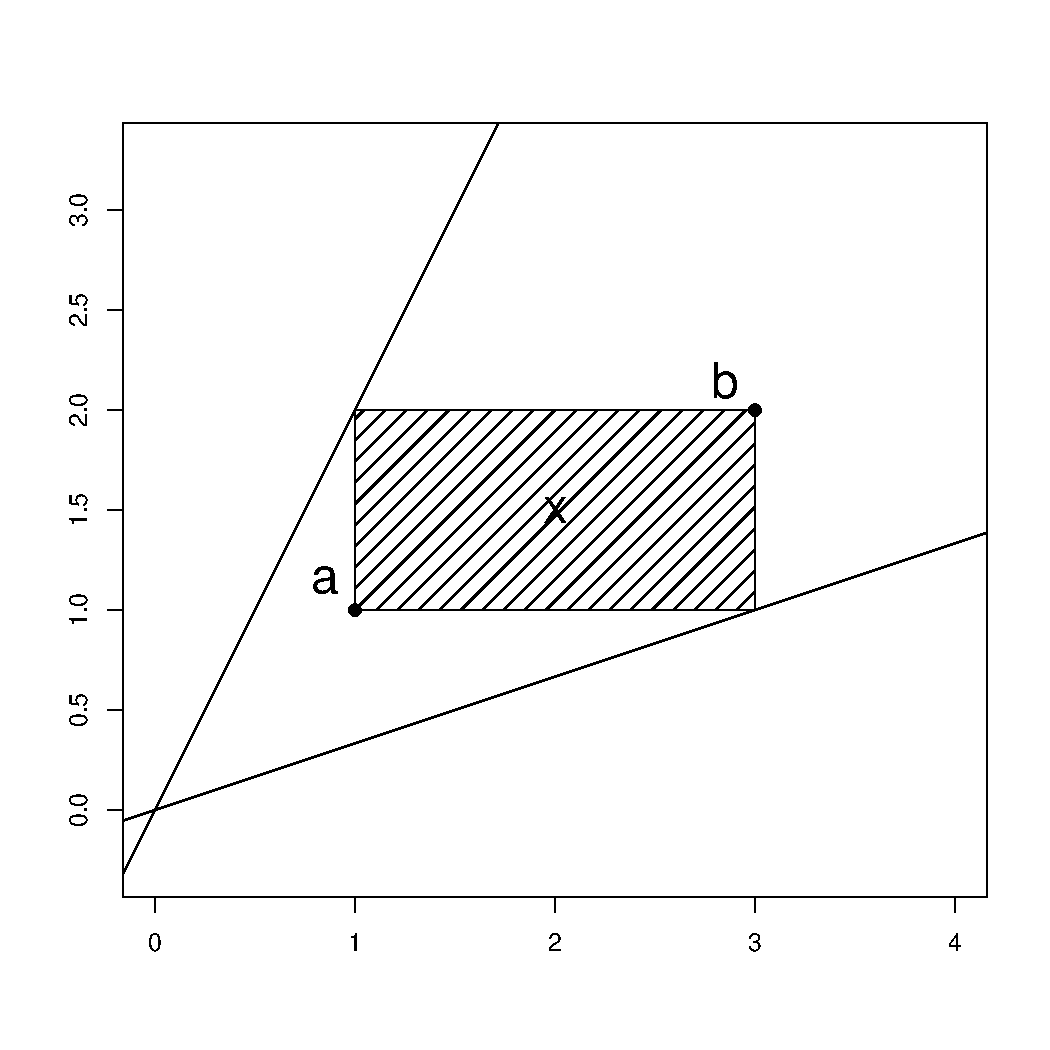
\includegraphics[scale=0.5]{constraints_x.pdf}}
\caption{При ограничениях вида $\bm{a}\leq\bm{x}\leq\bm{b}$ и отсутствии ограничений на вектор $\bm{y}$ прямая аппроксимации должна пересекать закрашенный прямоугольник.}
\label{fig:constraints_for_x}
\end{figure}

Чтобы сформулировать эту задачу в терминах приближенной факторизации (аппроксимации) матриц, сформируем матрицу $\bm{A}$ с векторами  $\bm{a}_{1},\ldots,\bm{a}_{n}$ в роли столбцов. Пусть $\bm{y}^{-}=(y_{j}^{-1})$ --- вектор-строка с положительными элементами. Тогда в общем случае задача приближения столбцов матрицы $\bm{A}$ при помощи векторов вида $y_{j}^{-1}\bm{x}$ есть задача одноранговой аппроксимации в форме \eqref{eq:factorization}.

%В метрике Евклида задача приближения точек при помощи прямой известна как задача полных наименьших квадратов (total least squares) и имеет смысл  множественной линейной регрессии в модели, где учитываются ошибки как в измерении зависимой переменной, так и в измерении независимых переменных. 
%Задача полных наименьших квадратов обычно решается при помощи $SVD$-разложения \cite{Golub1980Analysis}. Чебышевское расстояние: \cite{Hladik2015Total}



\subsubsection{Пример приближения множества точек на плоскости}
Рассмотрим двумерную задачу приближения множества точек при помощи прямой на моделированном примере. Сгенерируем сто двумерных векторов, имеющих нормальное распределение. %Обозначим абсциссы этих точек через $s_{i}$, а ординаты --- через $t_{i}$. Первые координаты двумерных точек распределены нормально со средним $3$ и стандартным отклонением $0.5$.
%Пусть справедлива модель $t_{i}=\beta(s_{i}+\delta_{i})+\varepsilon_{i}$ для $i=1,\ldots,m$, $\delta_{i}$ и $\varepsilon_{i}$ --- шум с распределением $\mathrm{Uniform}(-0.1,0.1)$ и $\mathrm{Uniform}(-0.2,0.2)$ соответственно.
На рисунке~\ref{fig:linenormnoiseuni} изображена прямая наилучшего приближения в $\log$-чебышевском смысле, полученная при помощи применения теорем из разделов~\ref{sec:SCAM},~\ref{sec:SCRM} настоящей главы, а также прямые наилучшего приближения для евклидовой ($L_{2}$) и манхэттенской ($L_{1}$) метрик.
%На рисунке~\ref{fig:linenormnoiseuni} представлен результат применения теорем главы~\ref{chap:PTO} к задаче приближения $100$ точек и его сравнение с результатами, минимизирующими евклидову ($L_{2}$) и манхэттенскую ($L_{1}$) метрики. 
\begin{figure}[h]
\center{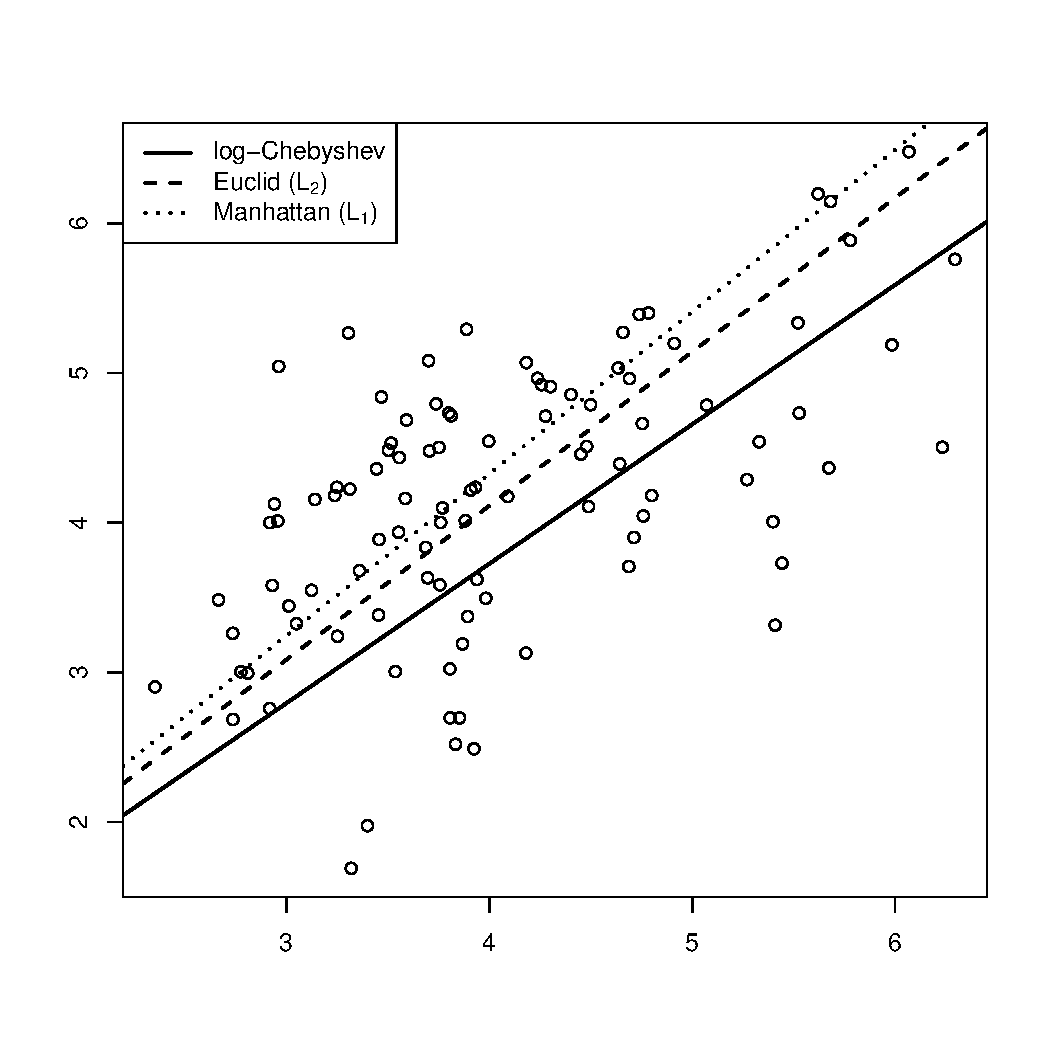
\includegraphics[scale=0.7]{norm100_3.pdf}}
\caption{Прямые наилучшего приближения для 100 нормально распределенных точек.}
\label{fig:linenormnoiseuni}
\end{figure}

%При проведении $1000$ экспериментов средняя абсолютная ошибка оценивания коэффициента $\beta$ составила $0.007111$, что можно сравнить со средней ошибкой  оценивания при минимизации расстояния Евклида, которая в таком случае составляет $0.009558$. При минимизации L1 ошибка в среднем $0.0117$

%При принятии решений в производственных сферах иногда приходится использовать методы экспертных оценок, при  которых решение принимается на основе агрегирования некоторого количества мнений экспертов.

%Методы обработки экспертных оценок во многом определяются природой самих оценок. Экспертные оценки разделяют на ординальные (ранговые) и кардинальные (количественные). В соответствии с этим выделяют ординальный и кардинальный подходы к обработке экспертных оценок. При ординальном подходе эксперт ранжирует альтернативы и задача принятия группового решения состоит в определении результирующих рангов альтернатив. Кардинальный подход обеспечивает решение более общей задачи определения количественных показателей значимости альтернатив.
%От кардинального подхода можно перейти к ординальному при помощи упорядочения объектов в соответствии с величинами показателей обобщенных оценок объектов.


%построение обобщенной оценки понятий и объектов на основе индивидуальных оценок экспертов;
%построение обобщенной оценки на основе парного сравнения объектов каждым из экспертов;

%При решении многих задач недостаточно упорядочения объектов по одному или группе показателей. Необходимо иметь числовые значения для каждого объекта, определяющие его предпочтение перед другими объектами. Наличие таких оценок позволит определить обобщенную оценку для всей группы экспертов.

%Определение согласованности мнений экспертов производится путем вычисления числовой меры, характеризующей степень близости индивидуальных мнений. Анализ значения меры согласования способствует выработке правильного суждения об общем уровне знаний по решаемой проблеме и выявлению группировок мнений экспертов.

\subsection{Приложение к задаче обработки экспертных оценок}\label{sec:PRO}
Практически во всех сферах, связанных с деятельностью человека, возникает необходимость применения экспертных оценок в процессе принятия решений.  
%%Задачи, связанные с принятием решений и ранжированием объектов, встречаются практически во всех областях человеческой деятельности. 
%Задача заключается в том, чтобы на множестве объектов (альтернатив), охарактеризованных некоторыми признаками, выбрать наилучший объект или ранжировать все объекты в порядке предпочтения.% Многие методы поиска наилучшей альтернативы также включают ранжирование всех рассматриваемых объектов согласно некоторому правилу.
Сущность метода экспертных оценок заключается в организации проведения экспертами оценки объектов (альтернатив) и последующей обработке полученных результатов. %Обобщенное мнение группы экспертов принимается как решение проблемы.
Задача обработки экспертных оценок состоит в том, чтобы по совокупности оценок нескольких экспертов получить обобщенную оценку для каждого объекта или ранжировать объекты в порядке предпочтения.

Подходы к обработке экспертных оценок во многом определяются природой исходных данных.  
Выделяют методы \cite{Tocenko2002Methods,Litvak1996Expert}, основанные на ранговом представлении оценок, и методы для оценок, описанных количественно. В первом случае эксперты ранжируют альтернативы и задача принятия группового решения состоит в определении результирующих рангов объектов.
В случае количественных экспертных оценок задача заключается в построении обобщенной оценки объектов на основе индивидуальных оценок экспертов. 
От количественного подхода можно перейти к ранговому при помощи упорядочения объектов в соответствии с величинами показателей обобщенных оценок альтернатив.

%Пусть $Q=\{q_{1},\ldots,q_{m}\}$ --- множество рассматриваемых объектов,
%$P=\{p_{1},\ldots,p_{n}\}$ --- множество измеренных в одной шкале признаков, по которым оценивается объект, либо множество экспертов, производящих оценку объектов по одному признаку.
%Каждому объекту $q_{i}$  соответствует оценка $a_{ij}$ по каждому признаку $p_{j}$. Из всех оценок объектов формируется матрица оценок $\bm{A}=(a_{ij})$.
%Задача ранжирования состоит в нахождении такой перестановки индексов объектов 
%$\begin{pmatrix}
%1 &2 &\ldots &m\\
%i_{1} &i_{2} &\ldots &i_{m}
%\end{pmatrix}$,
%что для всех $i_{k}$, $i_{l}$ из неравенства $i_{k}>i_{l}$ следует $q_{i_{k}}\succ q_{i_{l}}$, где последнее отношение будем понимать в смысле "объект $q_{i_{k}}$ лучше (предпочтительнее), чем $q_{i_{l}}$".

%В основе большинства методов решения задачи ранжирования лежит использование не количественных исходных данных (оценок объектов), а их порядковых соотношений (рангов). Такой подход однако не учитывает информацию о степени различия объектов по данным характеристикам (насколько один объект количественно лучше другого), к тому же обычно не допускает равенства рангов для разных объектов в одном признаке (или экспертном мнении). Ниже будет рассматриваться обобщение подхода к ранжированию объектов на основе матриц оценок, содержащих количественные характеристики объектов.

В статье \cite{Artamonov2016Group} задача ранжирования с оценками экспертов в виде рангов решается при помощи аппроксимации матрицы оценок одноранговой матрицей рангов, все столбцы которой одинаковы (матрица непротиворечивого ранжирования). 
%Тогда каждый столбец матрицы $\bm{A}$ определяет некоторую перестановку индексов объектов в соответствии с их предпочтительностью.
 %В этой работе применяется подход на основе аппроксимации матрицы оценок при помощи одноранговой матрицы рангов, все столбцы которой одинаковы (матрицы непротиворечивого ранжирования).
В настоящем разделе применяется распространение этого подхода на случай количественных оценок. Матрица, наилучшим образом согласованная со всеми векторами оценок, в таком случае ищется среди всех одноранговых матриц с одинаковыми столбцами над полем положительных вещественных чисел. Такая матрица полностью определяется вектором обобщенных (или согласованных) оценок. %, который обычно называют вектором обобщенных (или согласованных) оценок.
Если оценки экспертов представлены в определенном диапазоне значений, 
% Если признакам соответствует некоторый диапазон значений, 
то осмысленно потребовать того же и от значений результирующего вектора.


%...
%вектор обобщенных оценок. В соответствии с обобщенными оценками объектов может быть проведено ранжирование.
%
%степень согласованности оценок.

\subsubsection{Решение задачи}
Пусть $n$ экспертов оценивают $m$ объектов. Обозначим через $a_{ij}$ результат оценки $i$-го объекта $j$-м экспертом. Совокупность всех оценок обычно представляется в виде матрицы оценок $\bm{A}=(a_{ij})$.
Задача поиска обобщенного вектора оценок эквивалентна задаче %Требуется решить задачу одноранговой
одноранговой аппроксимации матрицы $\bm{A}$ при помощи матрицы с одинаковыми столбцами.

В терминах задачи факторизации с ограничениями \eqref{eq:factorization} условие равенства столбцов соответствует требованию выполнения равенства $y_{j}=1$ для всех $j=1,\ldots,n$, то есть равенства вектора $\bm{y}$ вектору из единиц. Чтобы значения матрицы аппроксимации принадлежали тому же диапазону, что и исходные признаки, на вектор $\bm{x}$ накладываются ограничения в виде неравенства $\bm{a}\leq\bm{x}\leq\bm{b}$ для заданных векторов $\bm{a}$, $\bm{b}$.

%Рассмотрим задачу нахождения всех положительных векторов $\bm{x}$, которые минимизируют $\log$-чебышевское расстояние между матрицей $\bm{A}$ и матрицей $\bm{x}\bm{y}^{-}$.

Так как ограничения в настоящей задаче определяют вектор $\bm{y}$ однозначно, для решения задачи одноранговой факторизации с ограничениями предпочтительнее применять теорему~\ref{th:row-regular}, в которой вектор $\bm{x}$ определяется двойным неравенством, зависящим от вектора $\bm{y}$. Сформулируем результат для этого частного случая.
\begin{corollary}
\label{cor:marks}
Пусть $\bm{A}$ --- положительная матрица оценок, $\mu$ --- спектральный радиус матрицы $\bm{A}\bm{A}^{-}$, $\bm{1}$ --- вектор размера $n$, состоящий из единиц. Пусть $\bm{a}$ --- вектор, $\bm{b}$ --- регулярный вектор такие, что $\bm{b}^{-}\bm{a}\leq 1$. Положим $r=(m+n)/2$ и введем обозначение
\begin{multline*}
\theta
=
\mu^{1/2}
\oplus
\bigoplus_{k=1}^{\lceil r\rceil}
\left(
\bm{b}^{-}\bm{A}(\bm{A}^{-}\bm{A})^{k-1}\bm{1}
\oplus
\bm{1}^{-}\bm{A}^{-}(\bm{A}\bm{A}^{-})^{k-1}\bm{a}
\right)^{1/(2k-1)}
\oplus
\\
\oplus
\bigoplus_{k=1}^{\lfloor r\rfloor}
\left(
\bm{b}^{-}(\bm{A}\bm{A}^{-})^{k}\bm{a}
\oplus
\bm{1}^{-}(\bm{A}^{-}\bm{A})^{k}\bm{1}
\right)^{1/(2k)}.
\end{multline*}
Тогда все векторы обобщенных оценок $\bm{x}$ в смысле минимизации $\log$-чебышевского расстояния определяются неравенством  % матрицы непротиворечивых оценок определяются вектором $\bm{x}$, где
\begin{equation*}
\bm{a}
\oplus
\theta^{-1}\bm{A}\bm{1}
\leq
\bm{x}
\leq
(\theta^{-1}\bm{1}^{-}\bm{A}^{-}\oplus\bm{b}^{-})^{-}.
\end{equation*}
\end{corollary}

%\subsubsection{Пример}\label{subsec:E1}
%Рассмотрим задачу оценки качества шести объектов на основе оценок восьми экспертов. Пусть каждый эксперт ставит каждому объекту в соответствие оценку от $1$ (самая низкая оценка) до $10$ (самая высокая оценка).  Из всех оценок можно сформировать матрицу $\bm{A}=(a_{ij})$, где элемент $a_{ij}$ есть оценка $i$-го объекта $j$-м экспертом. 
%
%Пусть матрица оценок имеет вид 
%\begin{equation*}
%\bm{A}
%=
%\begin{pmatrix}
%7 &7 &6 &8 &5 &7 &7 &8\\
%9 &6 &9 &9 &8 &8 &9 &7\\
%7 &6 &7 &7 &6 &6 &7 &6\\
%4 &4 &4 &5 &3 &4 &4 &5\\
%8 &8 &9 &10 &8 &8 &8 &9\\
%2 &2 &3 &2 &3 &3 &3 &3
%\end{pmatrix}.
%\end{equation*}
%
%Положим
%\begin{equation*}
%\bm{a}
%=
%\begin{pmatrix}
%1\\1\\1\\1\\1\\1
%\end{pmatrix},
%\qquad
%\bm{b}
%=
%\begin{pmatrix}
%10\\10\\10\\10\\10\\10
%\end{pmatrix}.
%\end{equation*}
%
%Спектральный радиус матрицы $\bm{A}\bm{A}^{-}$ равен $\mu=\sqrt{10}/2\approx 1.581$.
%
%Минимум в задаче тропической оптимизации с ограничениями равен $\theta=\sqrt{15}/3\approx 1.291$.
%
%Применим следствие~\ref{cor:marks} к решению задачи нахождения матрицы непротиворечивых оценок.  Все решения задачи можно представить в форме
%\begin{equation*}
%\begin{pmatrix}
%6.197\\6.971\\5.422\\3.873\\7.746\\2.324
%\end{pmatrix}
%\approx
%\frac{\sqrt{15}}{5}
%\begin{pmatrix}
%8\\9\\7\\5\\10\\3
%\end{pmatrix}
%\leq\bm{x}\leq
%\frac{\sqrt{15}}{5}
%\begin{pmatrix}
%25/3\\10\\10\\5\\50/\sqrt{15}\\10/3
%\end{pmatrix}
%\approx
%\begin{pmatrix}
%6.455\\7.746\\7.746\\3.873\\10\\2.582
%\end{pmatrix}
%.
%\end{equation*}

%Из полученного решения можно сделать вывод о том, что объект $q_{5}$ является наилучшим, а объект $q_{6}$ --- наихудшим. Объект $q_{4}$ занимает пятое место в порядке предпочтений. Отношения между объектами $q_{1}$, $q_{2}$, $q_{3}$ определены неоднозначно.
%Тогда результат можно записать в виде $q_{5}\succ (q_{1},q_{2},q_{3})\succ q_{4}\succ q_{6}$, причем $q_{2}\succ q_{1}$.

%Сравним полученный результат с некоторыми стандартными методами принятия решений. 

%Метод Борда: Для каждого критерия за первое место определяем альтернативе одно очко, за второе --- два, за третье --- три. Затем очки суммируются и наиболее предпочтительным с точки
%зрения этого метода становится объект, набравший минимальное количество очков.
\subsubsection{Пример}\label{subsec:E1}
Рассмотрим задачу оценки качества четырех объектов на основе оценок восьми экспертов. Пусть каждый эксперт ставит каждому объекту в соответствие оценку от $1$ (самая низкая оценка) до $10$ (самая высокая оценка).  %Из всех оценок можно сформировать матрицу $\bm{A}=(a_{ij})$, где элемент $a_{ij}$ есть оценка $i$-го объекта $j$-м экспертом. 
Предположим, что матрица оценок имеет вид 
%Рассмотрим пример, демонстрирующий разницу между применением различных метрик к аппроксимации.
\begin{equation*}
\bm{A}=
\begin{pmatrix}
7 &8 &8 &7 &8 &9 &7 &7\\
5 &6 &6 &6 &6 &5 &6 &4\\
8 &8 &9 &9 &9 &9 &4 &8\\
5 &4 &6 &5 &5 &4 &5 &6
\end{pmatrix}
\end{equation*}

В соответствии с обозначенными ограничениями на допустимые значения положим
\begin{equation*}
\bm{a}
=
\begin{pmatrix}
1\\1\\1\\1
\end{pmatrix},
\qquad
\bm{b}
=
\begin{pmatrix}
10\\10\\10\\10
\end{pmatrix}.
\end{equation*}

Применим следствие~\ref{cor:marks} к решению задачи нахождения обобщенного вектора оценок.
Минимум в задаче тропической оптимизации с ограничениями равен $\theta=3/2$.
 Все решения задачи можно представить в форме
\begin{equation*}
\begin{pmatrix}
6\\4\\6\\4
\end{pmatrix}
\leq
\bm{x}
\leq
\begin{pmatrix}
10\\6\\6\\6
\end{pmatrix}.
\end{equation*}

Обозначим объекты, которым соответствуют строки матрицы оценок, через $q_{1}$, $q_{2}$, $q_{3}$, $q_{4}$. 
В соответствии с полученным множеством обобщенных значений можно ранжировать объекты следующим образом: $q_{1}\succ q_{3}\succ q_{2}\sim q_{4}$.

%При этом $L_{1}$-метрику минимизирует вектор
%\begin{equation*}
%\bm{x}
%=
%\begin{pmatrix}
%7\\6\\8.5\\5
%\end{pmatrix}.
%\end{equation*}
%
%$L_{2}$-метрику минимизирует 
%\begin{equation*}
%\bm{x}
%=
%\begin{pmatrix}
%7.5\\5.5\\8\\5
%\end{pmatrix}.
%\end{equation*}
%
%log-чебышевское расстояние есть смысл применять в задачах, когда отдельные наблюдения имеют большую важность. Например, если объекты --- производственные станки, а признаки --- оценки отдельных деталей. Низкая оценка отдельной детали может означать брак и непригодность станка, даже если в целом остальне детали хорошие.
%
%
%Так как аппроксимация в $\log$-чебышевском смысле часто дает большое множество решений, можно использовать подход, использующий последовательно несколько метрик.
%
%\begin{equation*}
%\bm{x}_{1}
%=
%\begin{pmatrix}
%7\\6\\6\\5
%\end{pmatrix},
%\qquad
%\bm{x}_{2}
%=
%\begin{pmatrix}
%7.5\\5.5\\6\\5
%\end{pmatrix}.
%\end{equation*}



\conclusion

В настоящей работе были получены следующие результаты:
\begin{itemize}
\item Описан переход от задачи одноранговой %$\log$-чебышевской 
аппроксимации (приближенной факторизации) положительных матриц с пропущенными значениями к задаче тропической оптимизации в терминах $\max$-алгебры, где целевая функция  определяется матрицей, нулевые значения которой соответствуют пропускам в исходной матрице. %для которой строится разложение. %, при котором пропущенные элементы матрицы доопределяются нулями% переходят в нулевые.
\item Для произвольного идемпотентного полуполя построено полное аналитическое решение задачи тропической оптимизации %, целевая функция которой определяется  квадратной матрицей. 
с квадратной матрицей. 
Решение представлено в двух различных формах: для произвольной ненулевой матрицы и для матрицы, которая не содержит нулевых столбцов (строк). % без нулевых столбцов (строк). %, регулярной по столбцам (строкам).
\item Полученные результаты тропической оптимизации применены к решению задачи одноранговой факторизации квадратных положительных матриц. 
Найден явный вид единственной аппроксимирующей матрицы для произвольной положительной матрицы второго порядка. 
Приведен численный пример решения задачи приближенной факторизации матрицы четвертого порядка, в котором минимальная погрешность аппроксимации достигается на некотором множестве матриц. 
%\begin{itemize}
%\item Представлено полное решение задачи одноранговой аппроксимации произвольной положительной двумерной матрицы в явном виде.
%\item Приведен численный пример решения задачи аппроксимации квадратной матрицы четвертого порядка.
%\end{itemize}
\item В терминах общего идемпотентного полуполя построено полное аналитическое решение задачи тропической оптимизации с ограничениями в виде линейных векторных неравенств. Решение приведено в двух формах: для произвольной прямоугольной матрицы и для прямоугольной матрицы без нулевых столбцов (строк).  %Решения записывается в явном виде в компактной векторной форме, удобной для дальнейшего анализа и непосредственных вычислений.
\item Полученные результаты применены к решению задачи одноранговой факторизации прямоугольных положительных матриц при наличии двусторонних ограничений на векторы в приближенном разложении. 
%Построены численные примеры решения задачи одноранговой факторизации с ограничениями для матриц с пропущенными значениями. 
Построены численные примеры факторизации матриц с пропусками при наложении ограничений на множество допустимых решений. 
%Для иллюстрации работы методов представлен пример аппроксимации произвольной матрицы и численный пример аппроксимации матрицы четвертого порядка.
%\item Рассмотрена задача тропической оптимизации с ограничениями на допустимые решения. Построены методы, дающие полные аналитические решения этой задачи в различных формах для общего случая прямоугольной матрицы.
%\item Приведено решение задач приближения множества точек и ранжирования объектов, основанное на применении полученных методов одноранговой факторизации.
Описаны приложения полученных результатов к решению задачи приближения множества точек и задачи обработки экспертных оценок. 
%Описана возможность применения полученных результатов к задаче приближения точек и обработки экспертных оценок.
%\item Полученные результаты позволяют находить все векторы приближенного мультипликативного разложения положительных матриц в явном виде в векторной форме, удобной для дальнейших исследований и непосредственных вычислений.
\end{itemize}


\bibliography{bibliography}

\end{document}
